\svnidlong
{$HeadURL: $}
{$LastChangedDate: $}
{$LastChangedRevision: $}
{$LastChangedBy: $}
\svnid{$Id: $}   

Three benchmark simplified models \cite{Carpenter:2013xra,Berlin:2014cfa} 
are recommended for Higgs+\MET searches:
\begin{itemize}
	\item A model where a leptophobic vector mediator ($Z_B^\prime$) is exchanged in the $s-$channel, 
	radiates a Higgs boson and decays into two DM particles (Fig.~\ref{fig:feyn_prod_monoH} (a));
    \item A model where a scalar mediator $S$ couples to the SM only 
	through the SM Higgs and decays to two DM particles (Fig.~\ref{fig:feyn_prod_monoH_S});
	\item A model where a vector \Zprime is produced resonantly and decays into a Higgs boson
	plus an intermediate heavy pseudoscalar particle $A^0$, in turn decaying into two DM particles (Fig. \ref{fig:feyn_prod_monoH} (b)). 
\end{itemize}

\begin{figure}[!h!tpd]
	\centering
	\unitlength=0.0046\textwidth
	\subfloat[\label{subfig:modelMonoHZprimeqq}]{
		\begin{feynmandiagram}[modelMonoHZprimeqq]
		\fmfleft{i1,i2}
		\fmfright{o1,o2,o3}
		\fmf{fermion}{i2,v1,i1}
		\fmflabel{\Large $q$}{i2}
		\fmflabel{\Large $\bar{q}$}{i1}
		\fmf{photon,label={\Large \Zprime}}{v1,v2}
		\fmf{photon,label={\Large \Zprime},label.angle=-100,label.distance=5}{v2,v3}
		\fmf{dashes}{v2,o3}
		\fmflabel{\Large $h$}{o3}
		% \fmfv{label={\Large $b,,\theta$},label.a=120,label.distance=5w}{v2}
		% \fmfv{label={\Large $y_{\chiDM}$},label.a=-45,label.distance=5w}{v3}
		\fmf{fermion}{o2,v3,o1}
		\fmflabel{\Large ${\bar{\chiDM}}$}{o1}
		\fmflabel{\Large ${\chiDM}$}{o2}
		\fmfdot{v1,v2,v3}
	\end{feynmandiagram}
	}
	%\\\vspace{\baselineskip}
	\subfloat[\label{subfig:modelMonoHSimplifiedA0}]{
	\begin{feynmandiagram}[modelMonoHSimplifiedA0]
		\fmfleft{i1,i2}
		\fmfright{o1,o2,o3}
		\fmf{fermion}{i2,v1,i1}
		\fmflabel{\Large $q$}{i2}
		\fmflabel{\Large $\bar{q}$}{i1}
		\fmf{photon,label={\Large \Zprime}}{v1,v2}
		\fmf{dashes}{v2,o3}
		\fmflabel{\Large $h$}{o3}
		\fmf{dots_arrow,label={\Large $A^0$},label.side=right}{v2,v3}
		\fmf{fermion,tension=2}{o2,v3,o1}
		\fmflabel{\Large ${\bar{\chiDM}}$}{o1}
		\fmflabel{\Large ${\chiDM}$}{o2}
		\fmfdot{v1}
	\end{feynmandiagram}
	}
	\caption
	{
		Feynman diagrams of leading order processes leading to Higgs+\MET events: 
                (a) %%% ref doesn't seem to work here
                a model with a vector mediator (\Zprime) 
		coupling with DM and with the Higgs boson $h$,
%\ref{subfig:modelMonoHZprimeqq}, %%% ref doesn't seem to work here
and
                (b) %%% ref doesn't seem to work here
		a 2HDM model with a new invisibly decaying pseudoscalar $A^0$ 
		from the decay of an on-shell resonance \Zprime giving rise to a Higgs+\MET signature
%~\ref{subfig:modelMonoHSimplifiedA0}
.
	}
	\label{fig:feyn_prod_monoH}
\end{figure}
		
\begin{figure}[!h!tpd]
	\centering
	\unitlength=0.0046\textwidth
	\subfloat[\label{subfig:modelMonoHbaryonicqq}]{
		\begin{feynmandiagram}[modelMonoHbaryonicqq]
			\fmfleft{i1,i2}
			\fmfright{o1,o2,o3}
			\fmf{fermion}{i2,v1,i1}
			\fmflabel{\Large $q$}{i2}
			\fmflabel{\Large $\bar{q}$}{i1}
			\fmf{dashes,label={\Large $h,,S$}}{v1,v2}
			\fmf{dashes,label={\Large $h,,S$},label.side=right}{v2,v3}
			\fmf{dashes}{v2,o3}
			\fmflabel{\Large $h$}{o3}
			\fmfv{label={$b,,\theta$},label.a=100,label.distance=3w}{v2}
			\fmfv{label={$y_{\chiDM}$},label.a=-45,label.distance=5w}{v3}
			\fmf{fermion}{o2,v3,o1}
			\fmflabel{\Large ${\bar{\chiDM}}$}{o1}
			\fmflabel{\Large ${\chiDM}$}{o2}
			\fmfdot{v1,v2,v3}
		\end{feynmandiagram}
	}\\\vspace{\baselineskip}
	\subfloat[\label{subfig:modelMonoHbaryonicgg}]{
		\begin{feynmandiagram}[modelMonoHbaryonicgg]
			\fmfleft{i1,i2}
			\fmfright{o1,o2,o3}
			\fmf{gluon}{i1,vt1}
			\fmf{gluon}{i2,vt2}
			\fmflabel{\Large $g$}{i2}
			\fmflabel{\Large $g$}{i1}
			\fmf{fermion,label={\Large $t$}}{vt1,vt2}
			\fmf{fermion}{vt2,v1,vt1}
			\fmf{dashes,label={\Large $h,,S$},label.side=right}{v1,v2}
			\fmf{dashes,label={\Large $h,,S$},label.side=right,label.d=5}{v2,v3}
			\fmf{dashes}{v2,o3}
			\fmflabel{\Large $h$}{o3}
			\fmfv{label={$b,,\theta$},label.a=120,label.distance=3w}{v2}
			\fmfv{label={$y_{\chiDM}$},label.a=-45,label.distance=5w}{v3}
			\fmf{fermion}{o2,v3,o1}
			\fmflabel{\Large ${\bar{\chiDM}}$}{o1}
			\fmflabel{\Large ${\chiDM}$}{o2}
			\fmfdot{v1,v2,v3}
		\end{feynmandiagram}
	}
	\subfloat[\label{subfig:modelMonoHbaryonicggS}]{
	\begin{feynmandiagram}[modelMonoHbaryonicggS]
		\fmfleft{i1,i2}
		\fmfright{o1,o2,o3}
		\fmf{gluon}{i1,vt1}
		\fmf{gluon}{i2,vt2}
		\fmflabel{\Large $g$}{i2}
		\fmflabel{\Large $g$}{i1}
		\fmf{fermion,label={\Large $t$}}{vt1,vt2}
		\fmf{fermion}{vt2,v2,v1,vt1}
		\fmf{dashes}{v2,o3}
		\fmflabel{\Large $h$}{o3}
		\fmf{dashes,label={\Large $h,,S$},label.side=right,label.d=5}{v1,v3}
		\fmfv{label={$y_{\chiDM}$},label.a=-45,label.distance=5w}{v3}
		\fmf{fermion}{o2,v3,o1}
		\fmflabel{\Large ${\bar{\chiDM}}$}{o1}
		\fmflabel{\Large ${\chiDM}$}{o2}
		\fmfdot{v1,v2,v3,vt1,vt2}
	\end{feynmandiagram}

	}
	\caption
	{
		Feynman diagrams of leading order processes leading to Higgs+\MET events for a model with a scalar mediator ($S$) 
		coupling with DM and with the Higgs boson $h$. 
	}
	\label{fig:feyn_prod_monoH_S}
\end{figure}

These models are kinematically distinct from one another, as shown in the comparison of the 
\MET spectra in Fig.~\ref{fig:METSimpMonoHiggs} for high and low masses of the pseudoscalar mediator. 
Figure~\ref{fig:METSimpMonoHiggs} (a) shows the \MET distribution 
for models with high mediator masses ($m_{S} = 1$~\tev, $m_{\Zprime} = 1$~\tev, $m_{A^0} = 1$~\tev)
and DM mass of either 50 ($Z_B'$ and $A^0$ models) or 65~\gev (scalar mediator model).
Figure~\ref{fig:METSimpMonoHiggs} (b)  shows the \MET distribution 
for models with low pseudoscalar mediator masses ($m_{Z_B'} = 100$~\gev, $m_{\Zprime} = 1$~\tev, $m_{A^0} = 100$~\gev)
and DM mass of 1~\tev for all models. 
	

\begin{figure}[hbpt!]
	\centering
	\subfloat[High mediator mass]{
		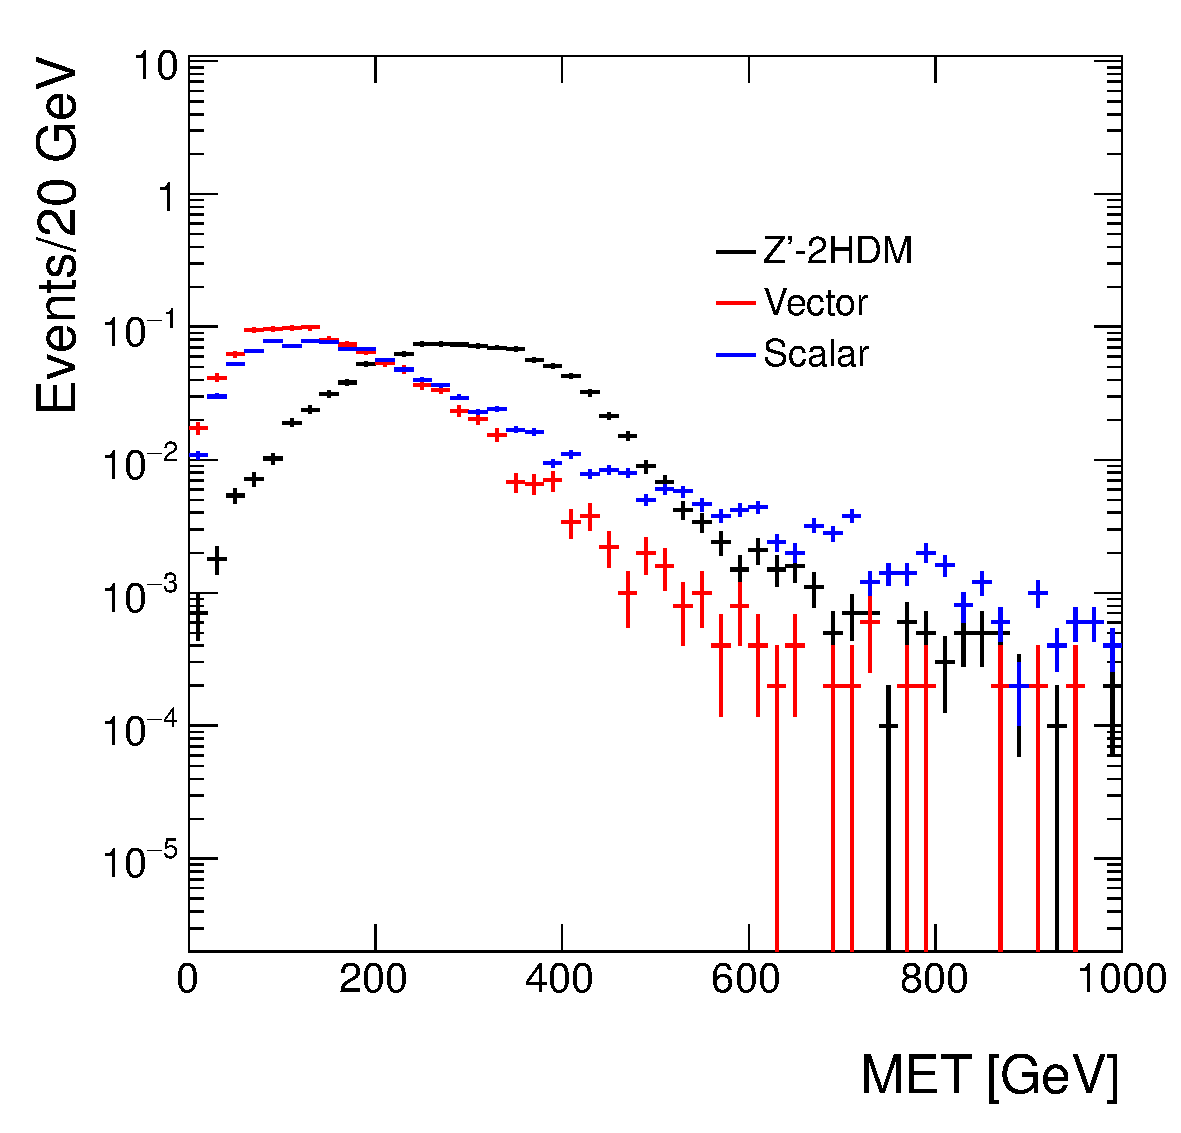
\includegraphics[width=0.47\linewidth]{figures/EW/monoH/models_cmp_MET_et_Log} \label{fig:met_cmp_high}
	}
	\subfloat[Low mediator mass]{
		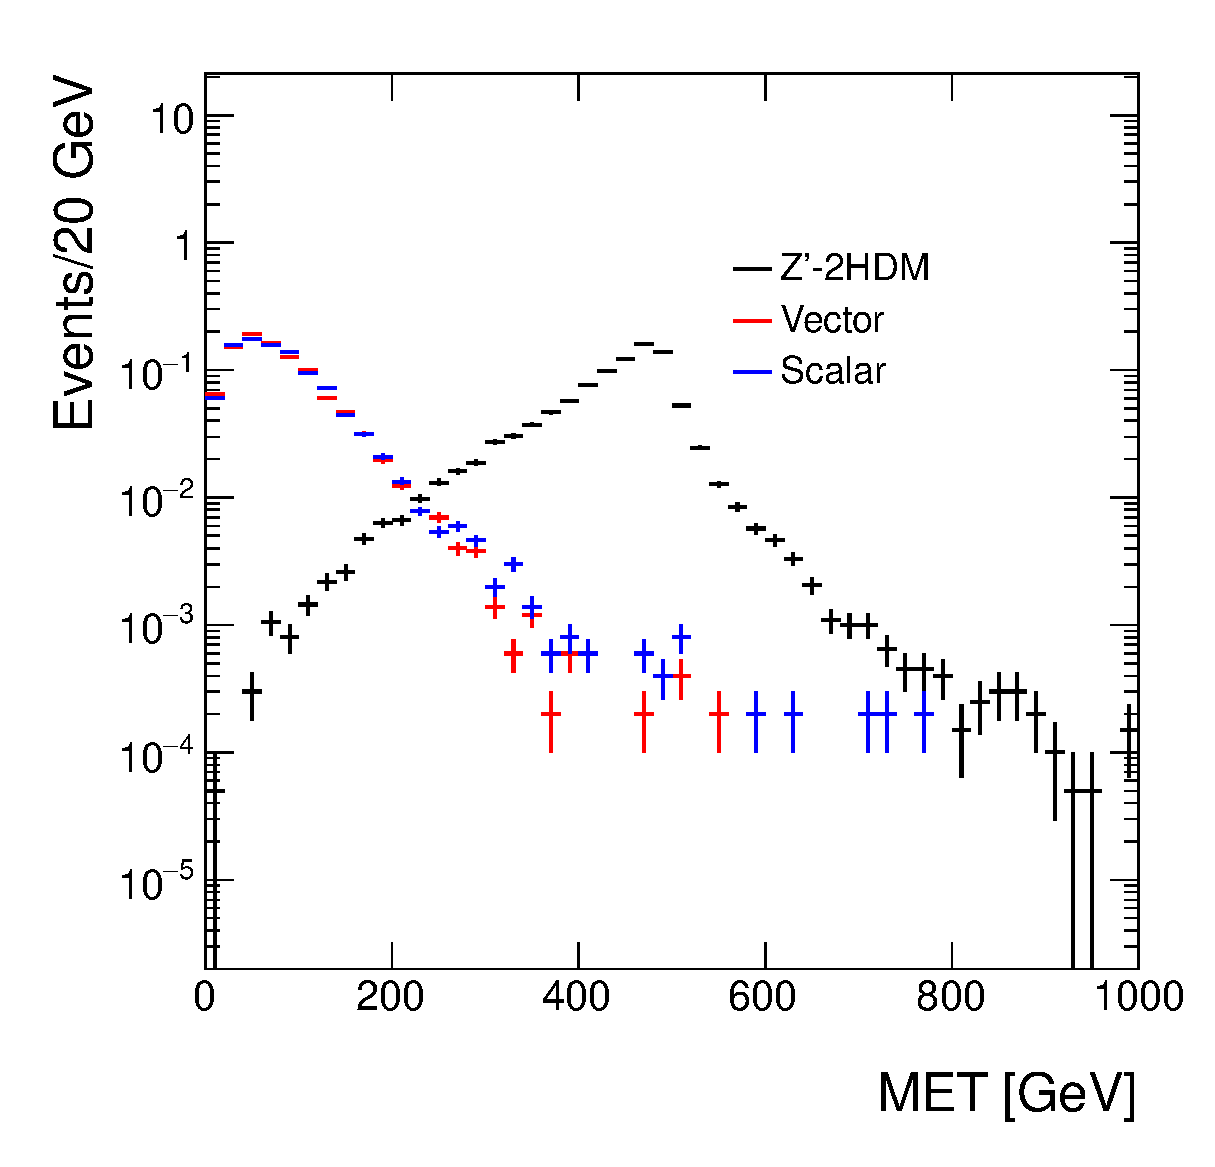
\includegraphics[width=0.47\linewidth]{figures/EW/monoH/models_cmp_low_MET_et_Log} \label{fig:met_cmp_low}
	}
	\caption{Comparison of the missing transverse momentum distributions at generator level in different 
		simplified models leading to a Higgs+\MET signature. The model parameter settings are detailed in the text.
		\label{fig:METSimpMonoHiggs}}
\end{figure}


\subsection{\MET+Higgs from a baryonic \Zprime}

The model shown in Fig.~\ref{fig:feyn_prod_monoH} (a)
postulates a new gauge boson \Zprime corresponding to a new $U(1)_B$ baryon 
number symmetry. The stable baryonic states included in this model are the DM candidate particles.
The mass of the \Zprime boson is acquired through a baryonic Higgs $h_B$, which mixes with the 
SM Higgs boson. The interactions between the \Zprime, the quarks and the DM are described by 
the following Lagrangian:   

\be \label{ZprimeDM}
%%\mathscr{
	L =  \gq  \bar q \gamma^\mu q  Z_\mu' +
%
%\left\{ \begin{array}{cc}
%	%i  \gDM  \chiDM^\dagger \smash{ \overset{\leftrightarrow}{\partial^\mu}}  \chiDM  \Zprime_\mu + \gDM^2 |\chiDM|^2 \Zprime_\mu Z^{\prime\mu} & {\rm scalar}  
	 \gDM  \bar\chiDM \gamma^\mu \chiDM Z_\mu' .
\ee

The quark couplings \gq are fixed to be equal to one third of the gauge coupling $g_B$, 
while the DM coupling to the \Zprime are proportional to the baryon number and to the gauge coupling 
($g_{\chiDM} = B g_B$). No leptonic couplings of the \Zprime are allowed, thus evading dilepton constraints. 
After incorporating the mixing of the baryonic and SM Higgs bosons, this model is 
is described by the following Lagrangian term at energies below $m_{\Zprime}$: 
 \be \label{U1Beft}
 L_{\rm eff} = - \frac{\gq \gDM }{m_{\Zprime}^2} \bar{q} \gamma^\mu q \bar\chiDM \gamma_\mu \chiDM \Big( 1 + \frac{g_{h \Zprime \Zprime} }{m_{\Zprime}^2} h \Big) \, ,
 \ee

The first term of this equation gives rise to a term that is equivalent to the 
radiation of a jet (or another EW gauge boson) in the initial state. 
The second term describes the interaction between the \Zprime and the SM Higgs boson,
via the coupling $g_{h \Zprime \Zprime} = \frac{m_{\Zprime}2 sin\theta}{v_B}$, where
$sin\theta$ is the mixing angle between the SM Higgs and the baryonic Higgs $h_B$, and $v_B$ is the
Baryonic Higgs vacuum expectation value. 

%TODO: 
%	1- Mention sensitivity difference wrt monojet? 
%	2- Mention why we don't consider the dark Z model?]}

\subsubsection{Parameter scan} 

The model is described by six parameters:
\begin{enumerate}
	\item the mediator mass \mmed, (also referred to as $m_{\Zprime}$)
	\item mass of dark matter, \mDM
	\item coupling of \Zprime mediator to dark matter, \gDM
	\item coupling of the mediator to quarks, \gq
	\item mixing angle between baryonic Higgs $h_B$ and the SM-like Higgs boson, $\sin\theta$
	\item coupling of the mediator to SM-like Higgs boson, $g_{h\Zprime \Zprime}$
\end{enumerate}
The width of the \Zprime mediator is calculated using all possible decays to SM particles (quarks) and to pairs of DM particles if kinematically allowed.

The dependence of the missing transverse momentum (\MET) on the model parameters 
is studied by varying the parameters one at a time. The variation of parameters 
other than \mMed and \mDM does not result in significant 
variations of the \MET spectrum, as shown in Figures~\ref{fig:metVectorCoupling}. 
Figure~\ref{fig:metVectorMass} shows that for an on-shell mediator, 
varying \mDM with the other parameters fixed does not affect the \MET distribution, while 
the distribution broadens significantly in the case of an off-shell mediator. 
For this reason, the same grid in \mmed, \mdm as for the vector mediator
of the jet+\MET search (Table~\ref{tab:mDMmMedScan_VA}) is chosen as a starting point. 
The coupling $g_{h\Zprime \Zprime}$, along with \gq and \gDM, are subject to perturbativity bounds:
$$\gq, \gDM < 4\pi $$ and $$  g_{h \Zprime \Zprime} < \sqrt{4\pi}m_{\Zprime}\sin\theta$$ 
The value $g_{h \Zprime \Zprime}/m_{\Zprime} = 1.0$ is chosen as a benchmark value for the generation 
of Monte Carlo samples since it maximizes the cross section (as shown in the following paragraph)
without violating the bounds. The mediator-DM coupling \gDM is fixed to 1, and  
the mediator-quark $g_{q}$ coupling is fixed to 1/3. 
The kinematic distributions do not change as a function of these parameters, so 
results for other values of  $g_{h \Zprime \Zprime}/m_{\Zprime}$, \gDM and \gq can be 
obtained through rescaling by the appropriate cross sections. 

Figs~\ref{fig:VectorHbb_100} and ~\ref{fig:VectorHbb_1000} show the kinematic distributions for the two leading jets
in the $H \to \bar b b$ decay channel, for two values of the mediator mass and varying the DM mass.  

Analyses should perform further studies, beyond those studies performed for the forum, to estimate the reach of the analysis with respect to all points in the grid and therefore decide on a smaller set of grid points to be generated.
%TODO: can we get sensitivity to all the points for all signatures?

\begin{figure}[hbpt!]
	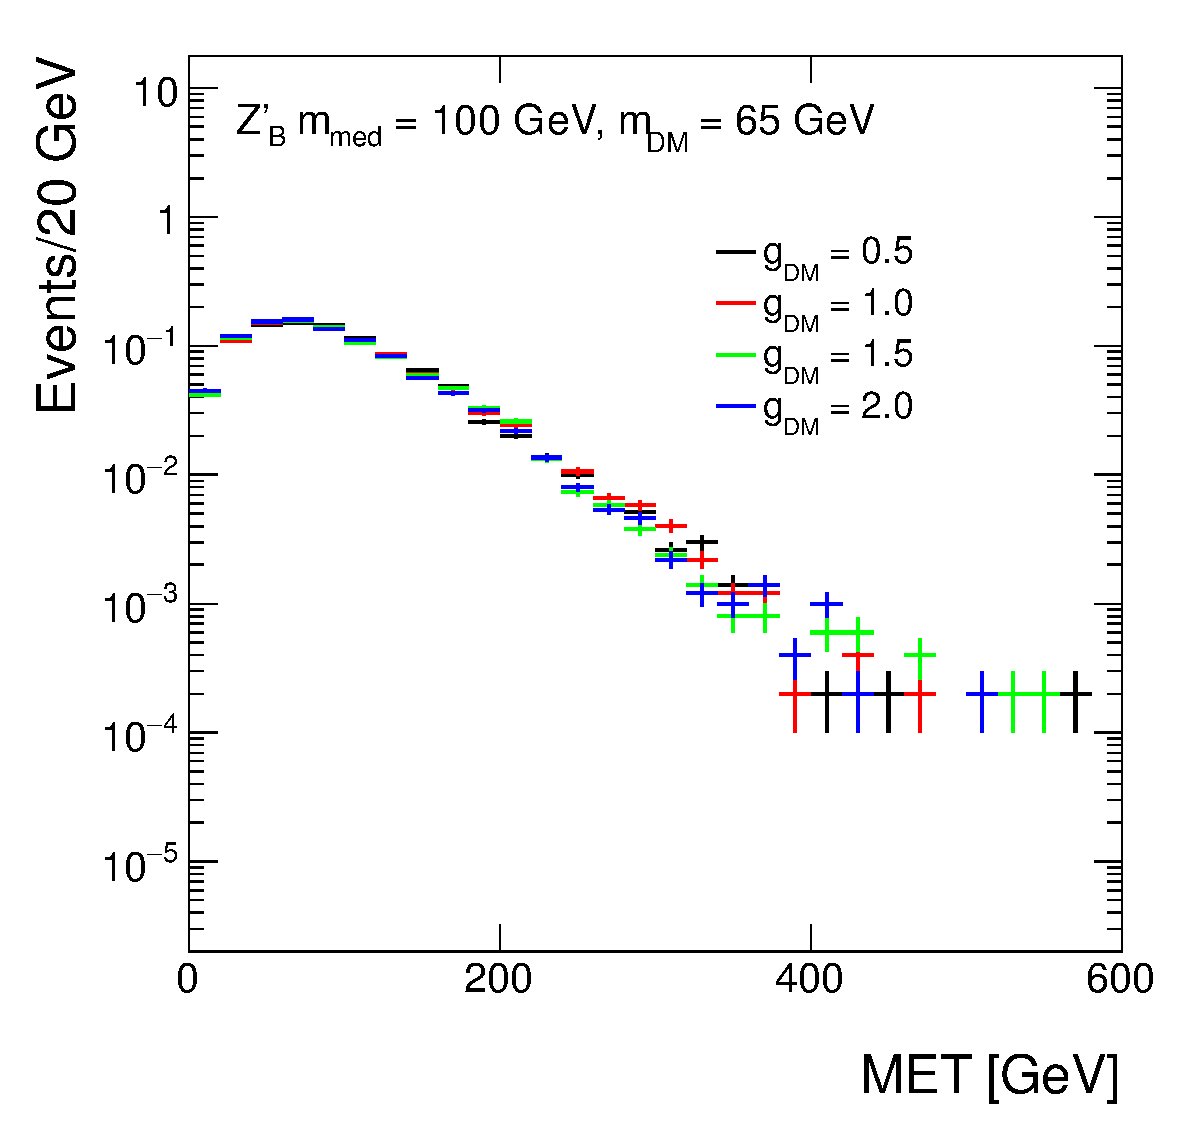
\includegraphics[width=0.49\linewidth]{figures/EW/monoH/z_gdm_MET_et_Log}
	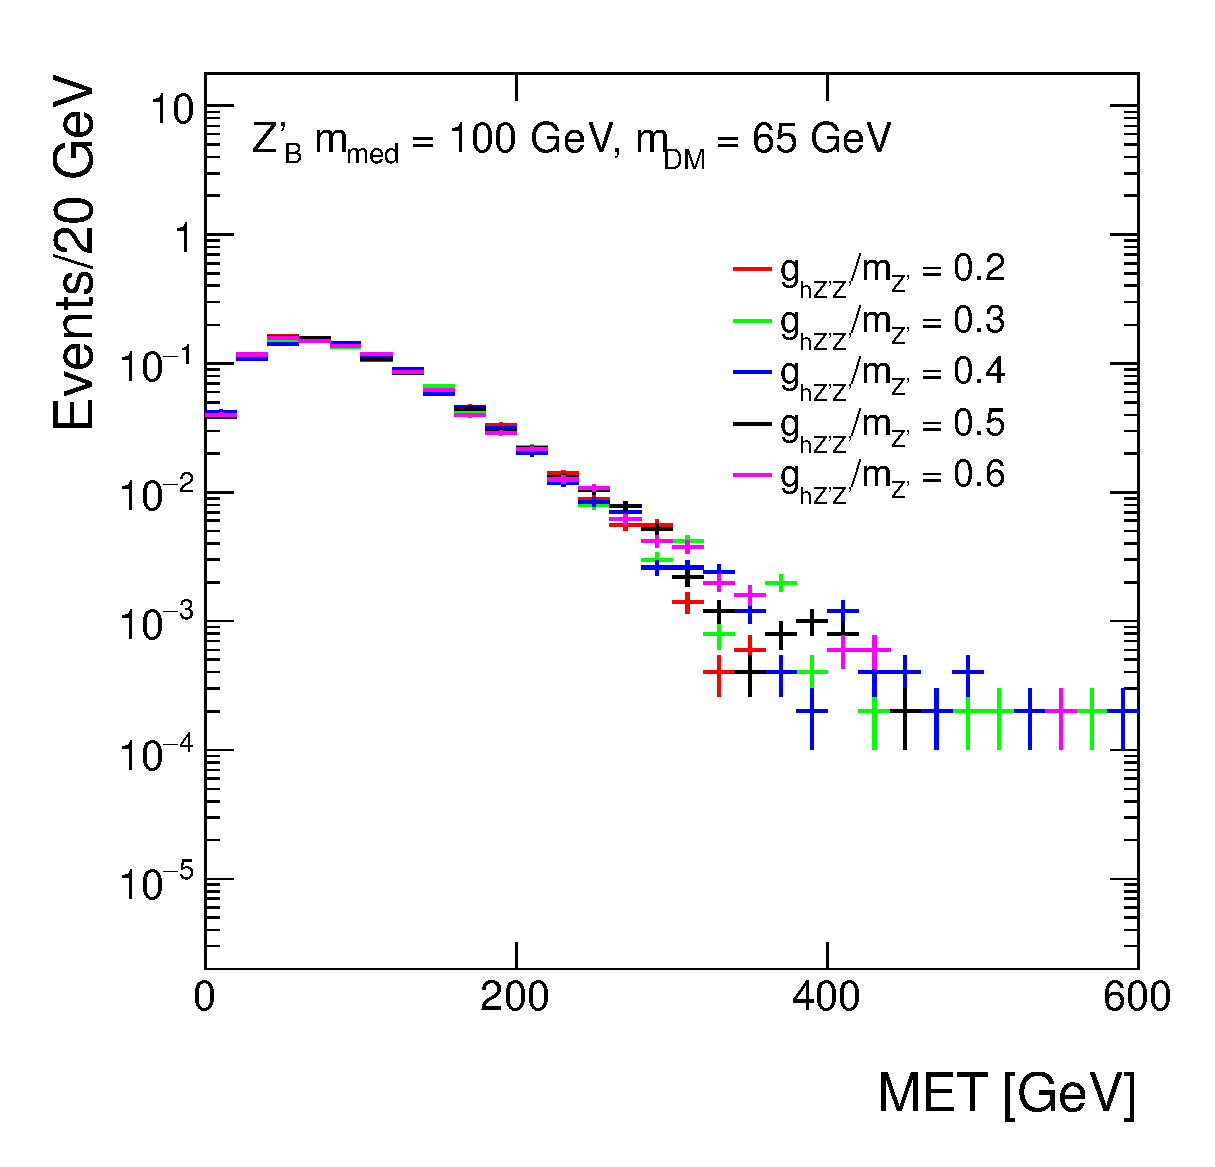
\includegraphics[width=0.49\linewidth]{figures/EW/monoH/z_ratio_MET_et_Log}
	\caption{Missing transverse momentum distributions at generator level in the vector 
		mediator scenario for different values of: the mediator-dark matter coupling \gDM (left),
		and the coupling between the mediator and the SM-like Higgs boson, scaled by the mediator mass, 
		$g_{h \Zprime \Zprime}/m_{\Zprime}$ (right).
		\label{fig:metVectorCoupling}}
\end{figure}

\begin{figure}[hbpt!]
	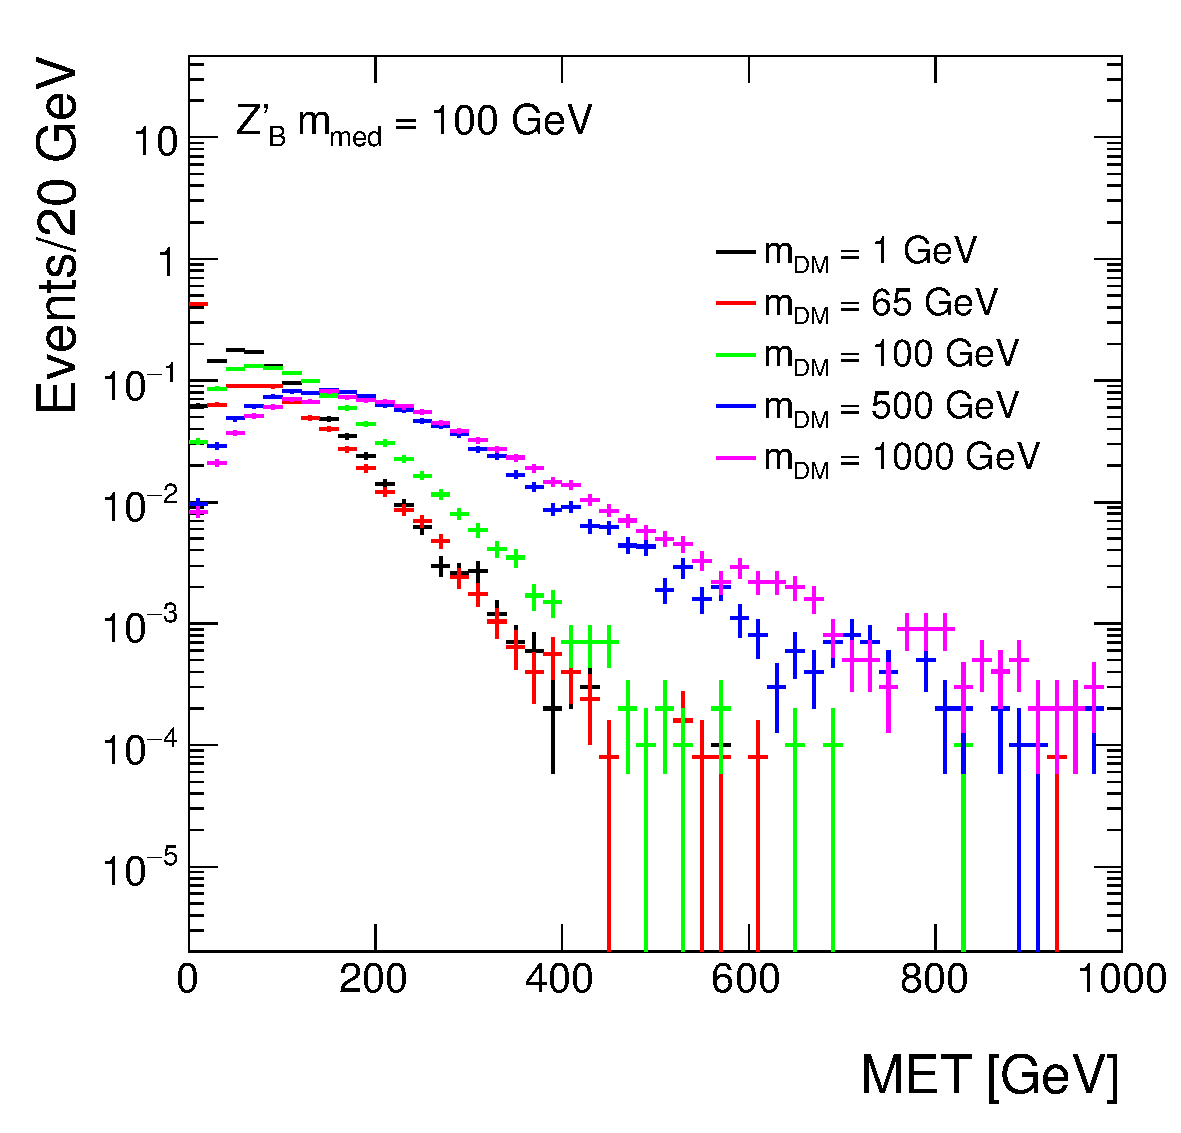
\includegraphics[width=0.49\linewidth]{figures/EW/monoH/zprime_100_MET_et_Log}
	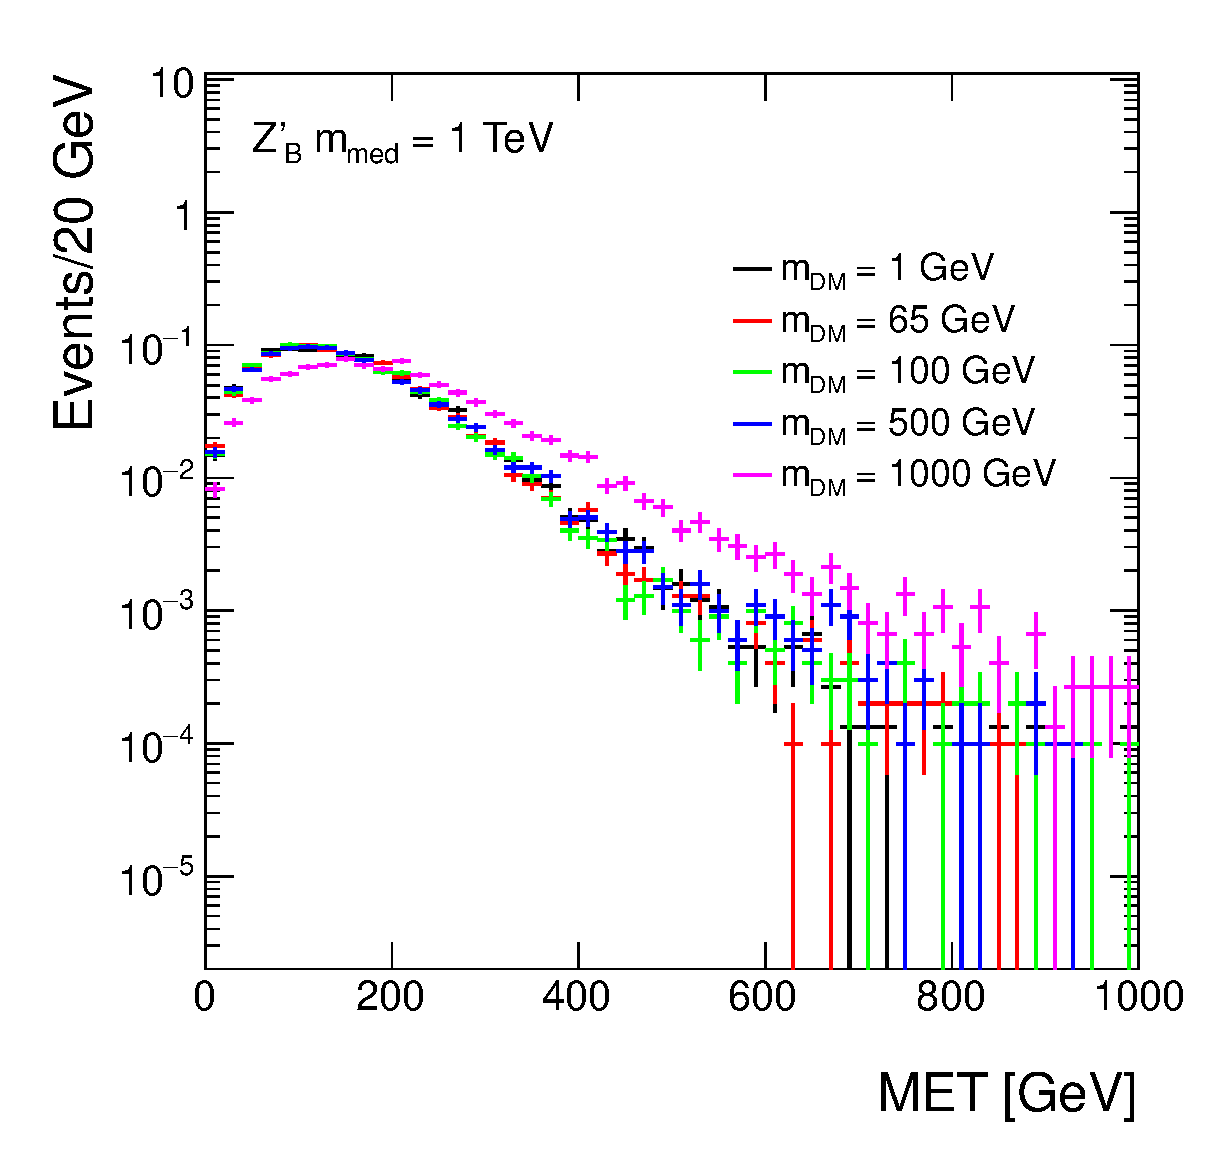
\includegraphics[width=0.49\linewidth]{figures/EW/monoH/zprime_1000_MET_et_Log}
	\caption{Missing transverse momentum distributions at generator level in the vector 
		mediator scenario: for different values of the dark matter mass \mDM 
		and a mediator mass of \mmed = 100~\gev (left) and \mmed = 1~\tev (right).
		\label{fig:metVectorMass} }
\end{figure}


\begin{figure}[hbpt!]
	\centering
	\subfloat[Leading $b-$jet transverse momentum]{
		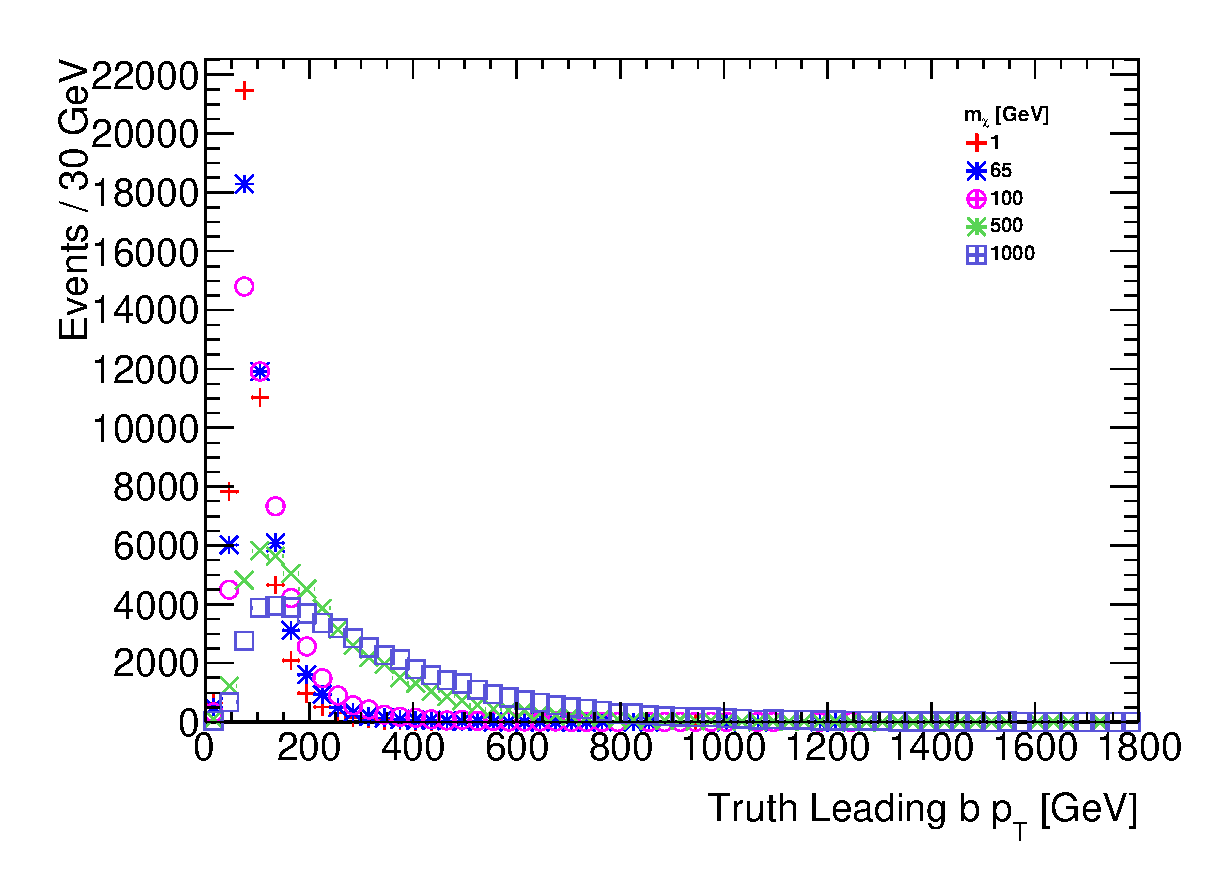
\includegraphics[width=0.47\linewidth]{figures/EW/monoH/zpzp100/truth_leading_b_pt} %\label{fig:met_cmp_high}
	}
	\hfill
	\subfloat[Leading $b-$jet pseudorapidity]{
		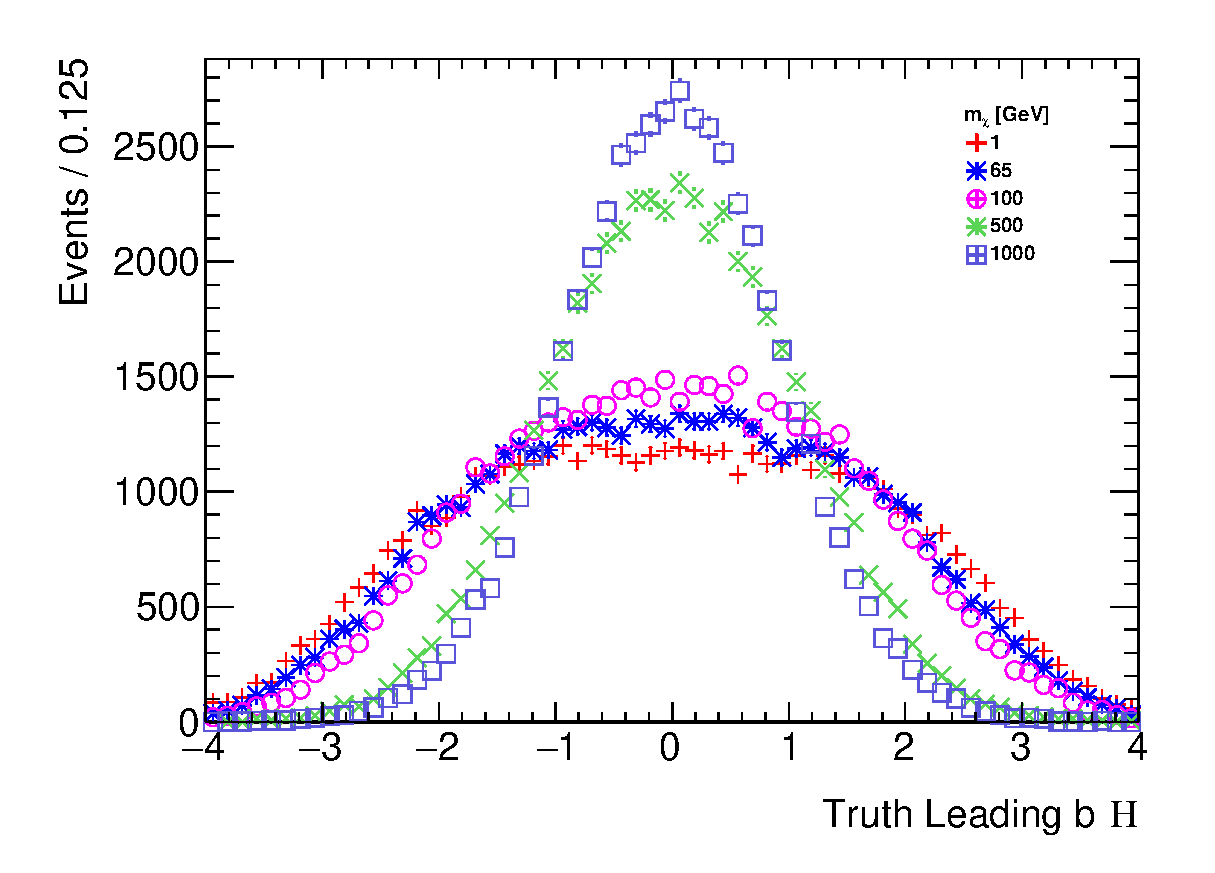
\includegraphics[width=0.47\linewidth]{figures/EW/monoH/zpzp100/truth_leading_b_eta} %\label{fig:met_cmp_low}
	}
%	\hfill
%	\subfloat[Leading $b-$jet transverse momentum]{
%		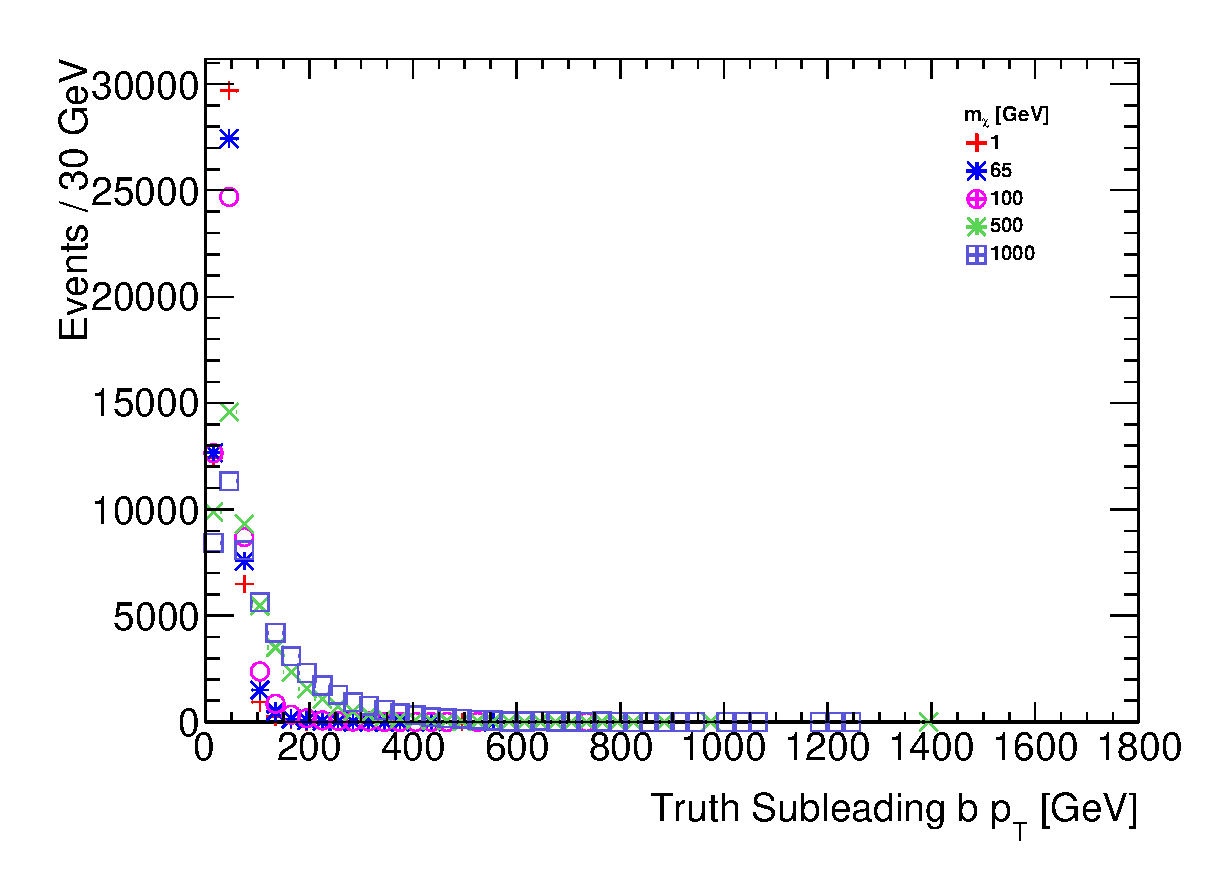
\includegraphics[width=0.47\linewidth]{figures/EW/monoH/zpzp100/truth_subleading_b_pt} %\label{fig:met_cmp_high}
%	}
%	\hfill
%	\subfloat[Leading $b-$jet pseudorapidity]{
%		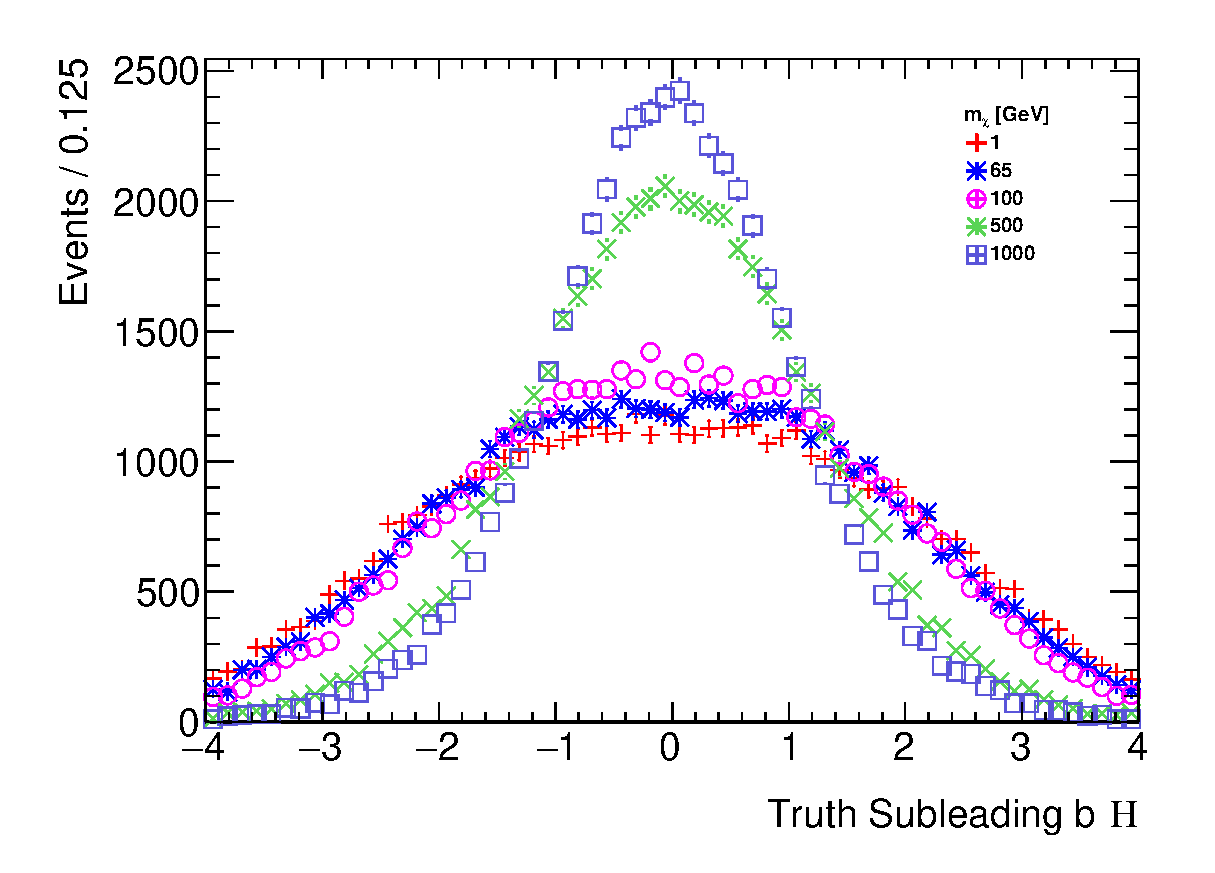
\includegraphics[width=0.47\linewidth]{figures/EW/monoH/zpzp100/truth_subleading_b_eta} %\label{fig:met_cmp_low}
%	}
	\hfill
	\subfloat[Angular distance between the two leading $b-$jets]{
		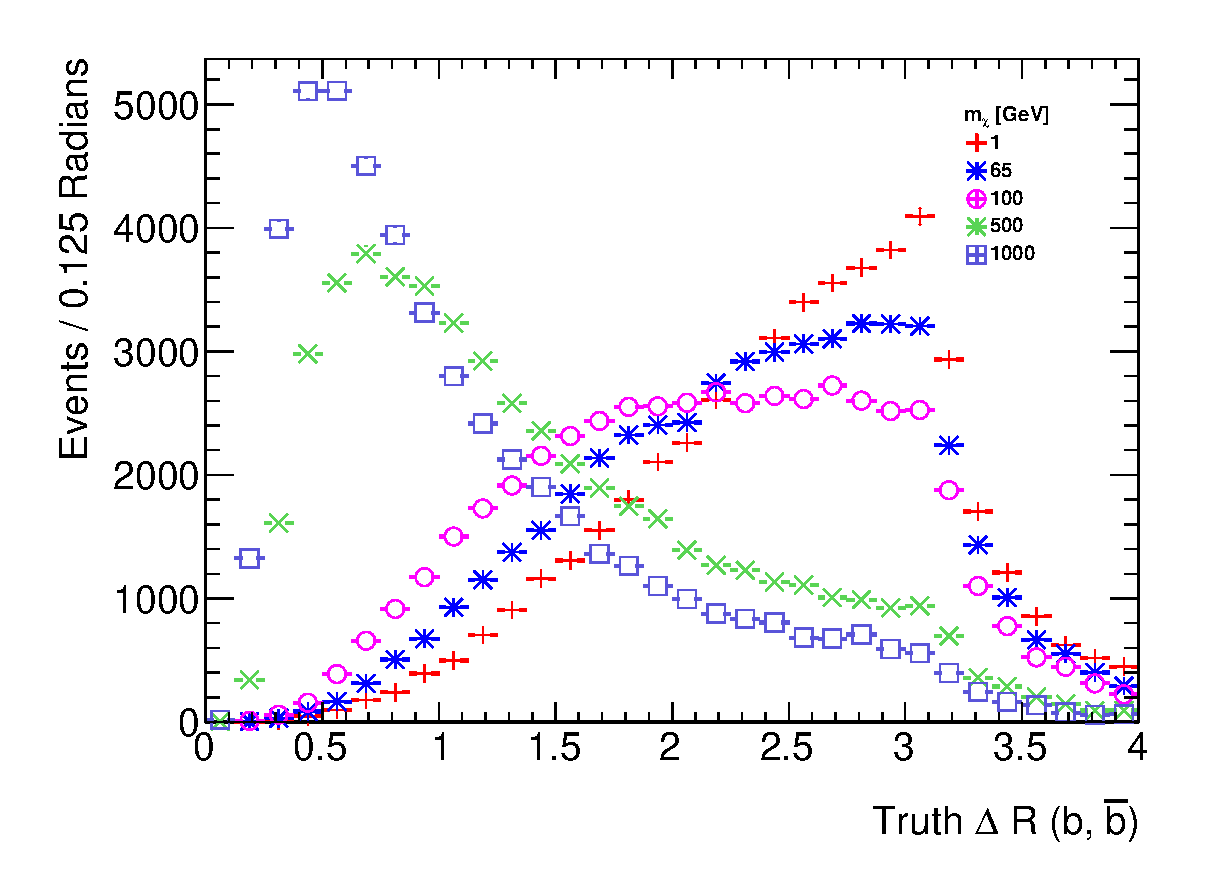
\includegraphics[width=0.47\linewidth]{figures/EW/monoH/zpzp100/truth_bb_deltar} %\label{fig:met_cmp_low}
	}
	\caption{Comparison of the kinematic distributions for the two leading $b-$jets (from the Higgs decay) in the vector \Zprime simplified model, 
		when fixing the \Zprime mass to 100~\gev and varying the DM mass. 
		\label{fig:VectorHbb_100}}
\end{figure}

\begin{figure}[hbpt!]
	\centering
	\subfloat[Leading $b-$jet transverse momentum]{
		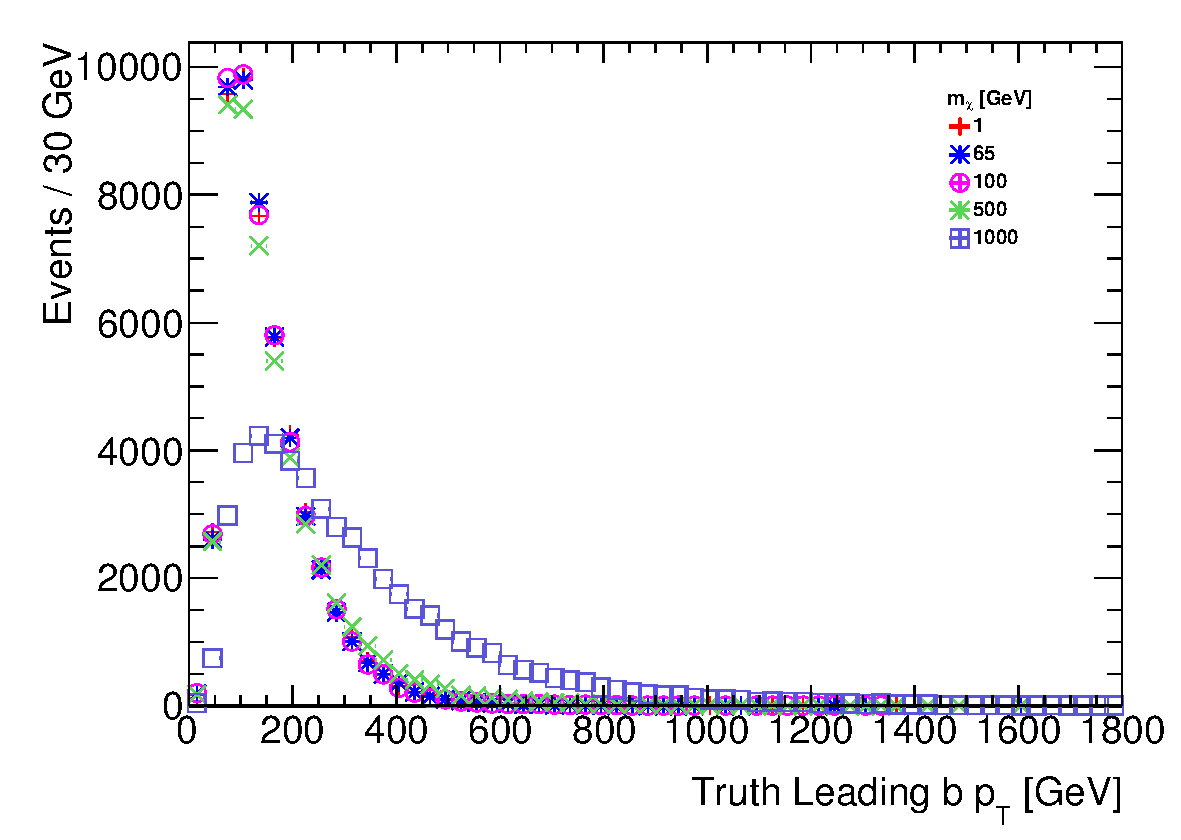
\includegraphics[width=0.47\linewidth]{figures/EW/monoH/zpzp1000/truth_leading_b_pt} %\label{fig:met_cmp_high}
	}
	\hfill
	\subfloat[Leading $b-$jet pseudorapidity]{
		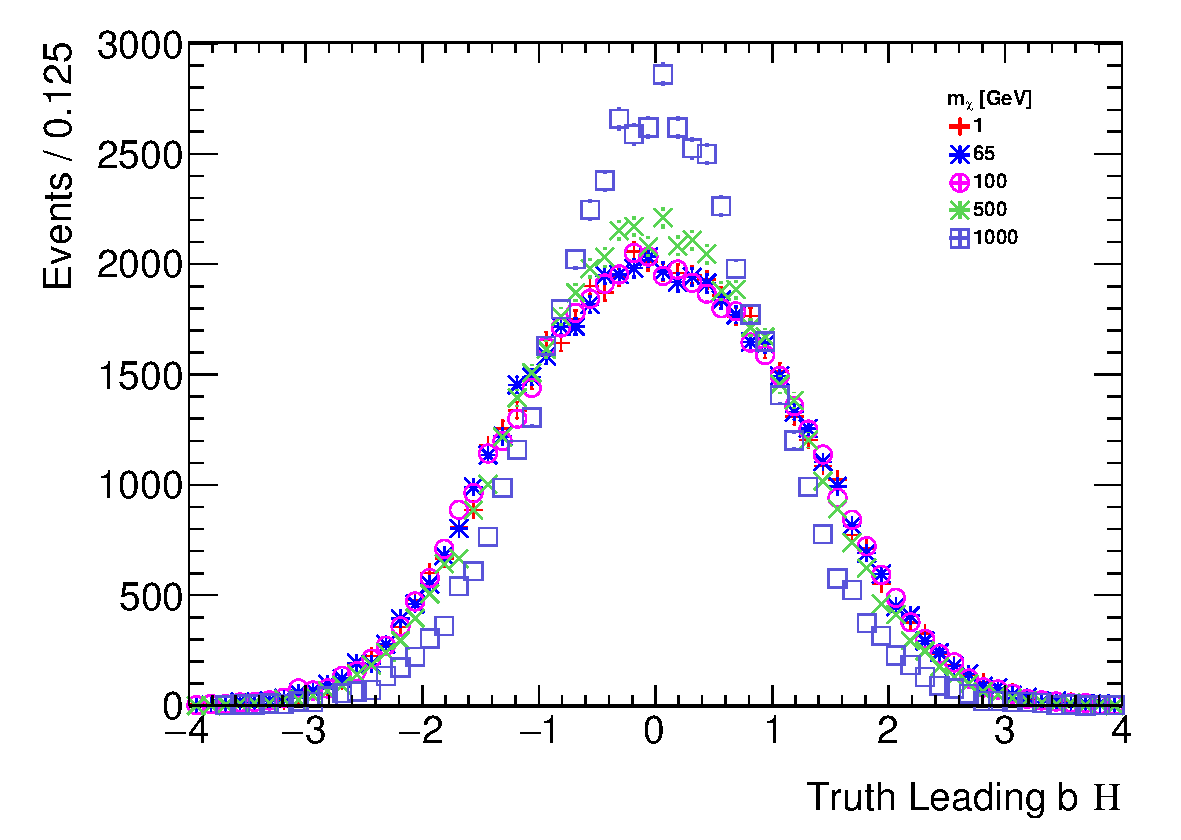
\includegraphics[width=0.47\linewidth]{figures/EW/monoH/zpzp1000/truth_leading_b_eta} %\label{fig:met_cmp_low}
	}
%	\hfill
%	\subfloat[Leading $b-$jet transverse momentum]{
%		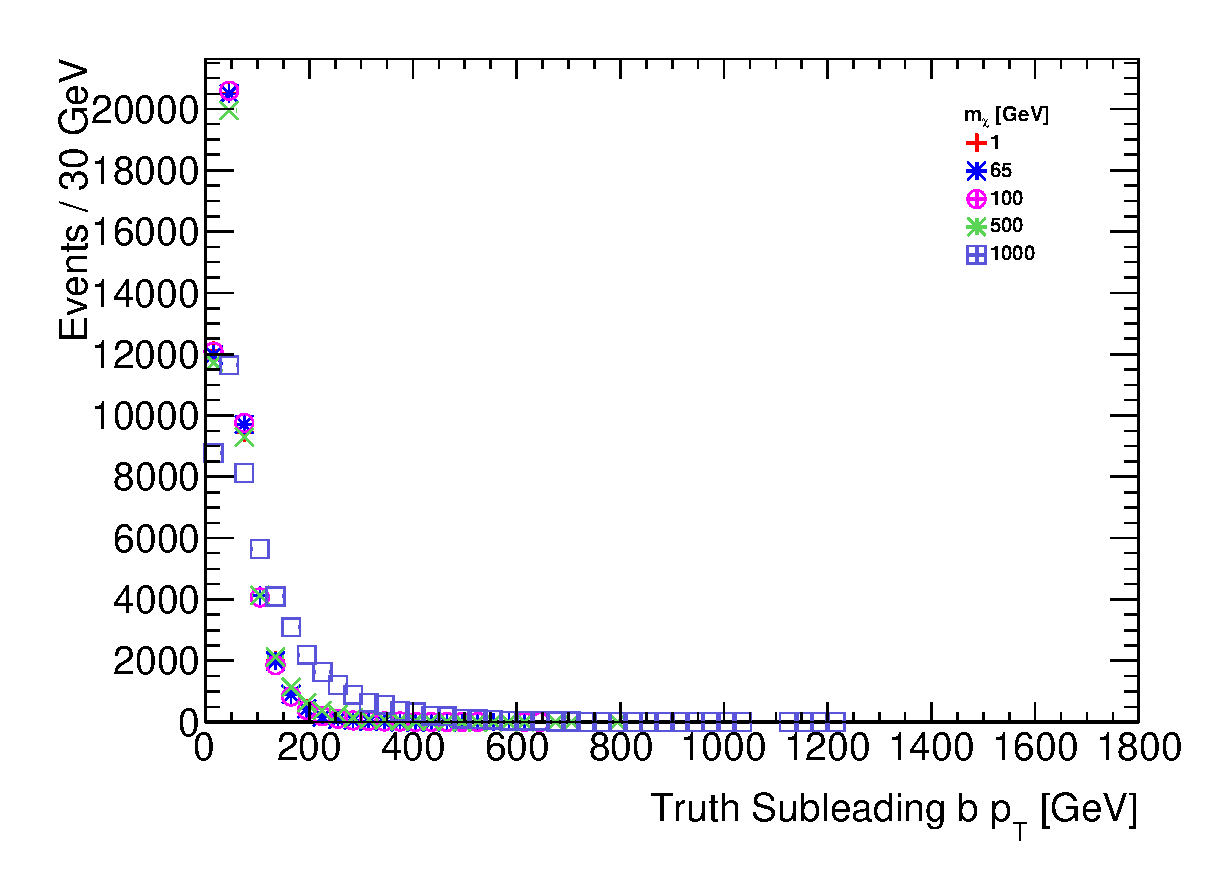
\includegraphics[width=0.47\linewidth]{figures/EW/monoH/zpzp1000/truth_subleading_b_pt} %\label{fig:met_cmp_high}
%	}
%	\hfill
%	\subfloat[Leading $b-$jet pseudorapidity]{
%		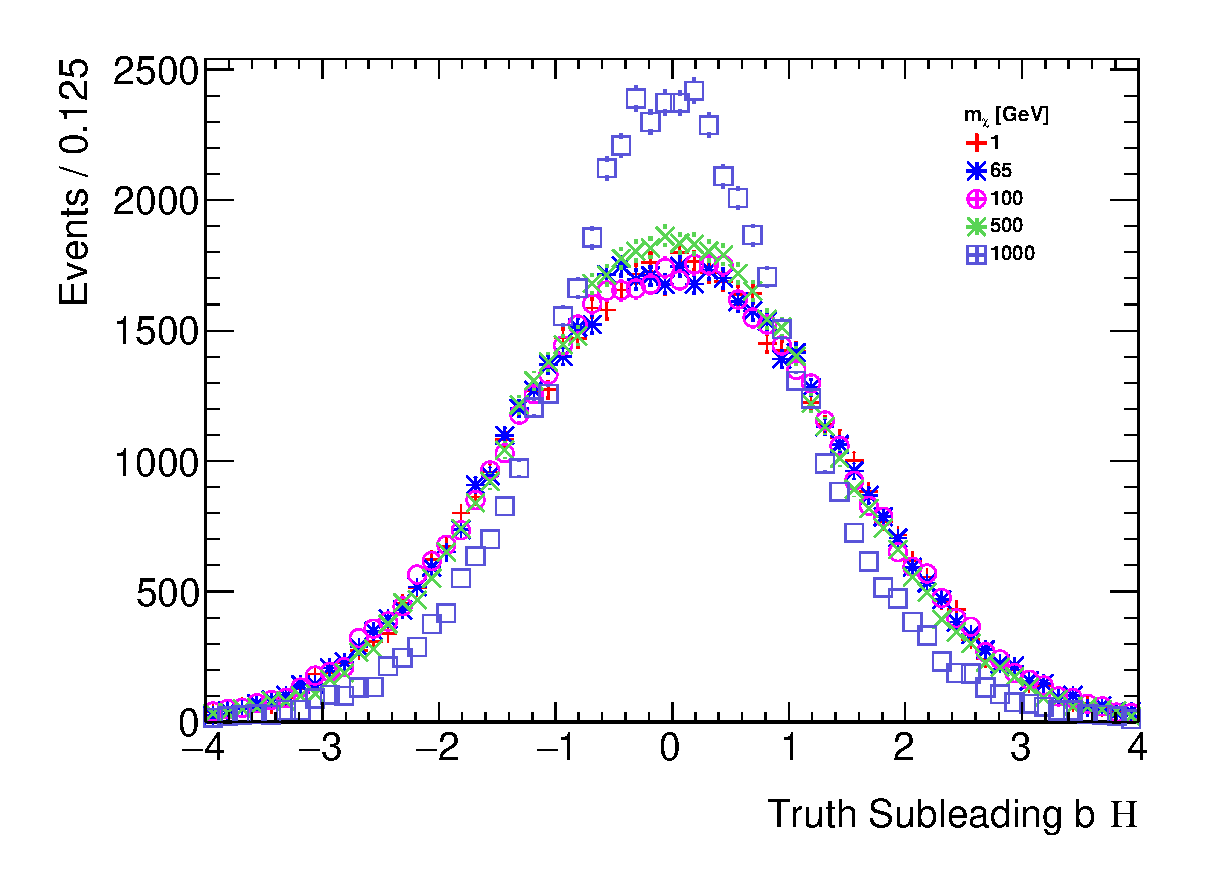
\includegraphics[width=0.47\linewidth]{figures/EW/monoH/zpzp1000/truth_subleading_b_eta} %\label{fig:met_cmp_low}
%	}
	\hfill
	\subfloat[\text{Angular separation of the two leading $b$-jets}]{
		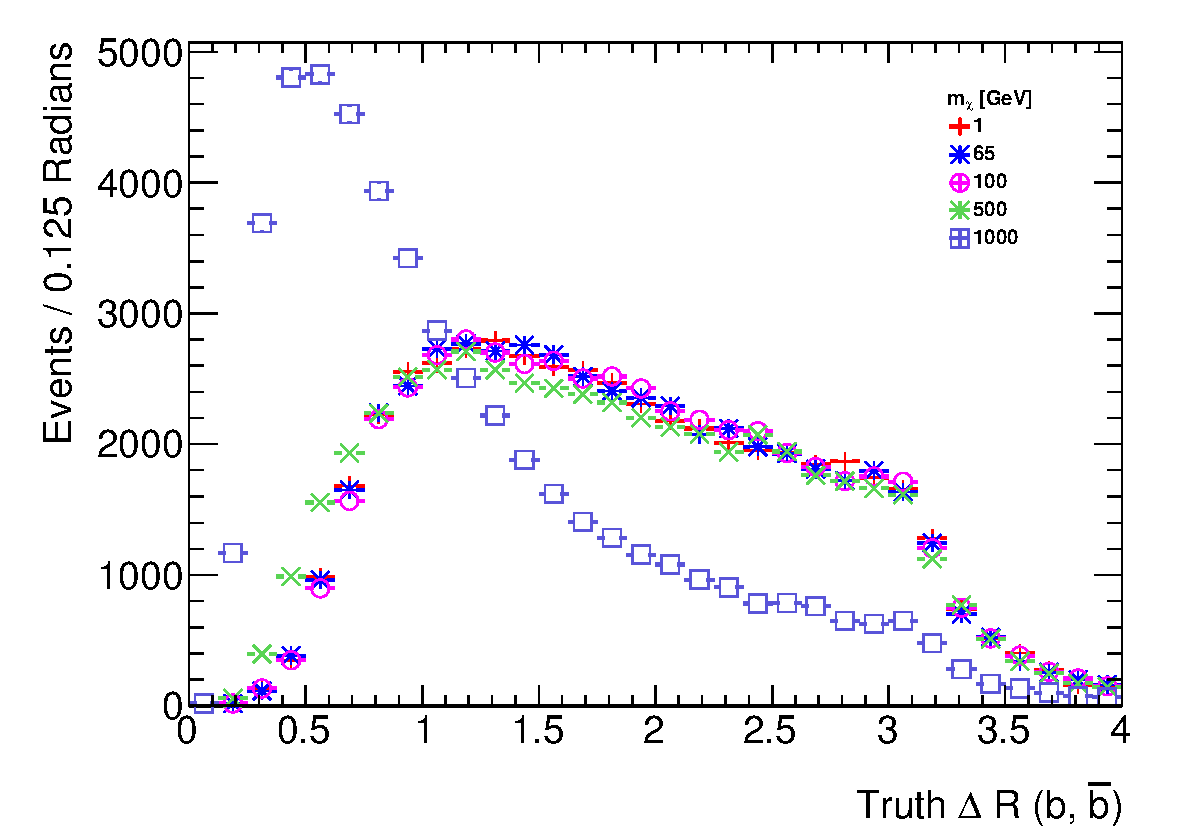
\includegraphics[width=0.47\linewidth]{figures/EW/monoH/zpzp1000/truth_bb_deltar} %\label{fig:met_cmp_low}
	}
	\caption{Comparison of the kinematic distributions for the two leading jets from the Higgs decay in the vector \Zprime simplified model, 
		when fixing the \Zprime mass to 1000~\gev and varying the DM mass. 
		\label{fig:VectorHbb_1000}}
\end{figure}

\subsubsection{Cross-section scaling}

The dependence of the cross section of the $pp \rightarrow H\chiDM\bar{\chiDM}+X$ process 
on $g_{h \Zprime \Zprime}$ is shown in Figure~\ref{fig:vectorXSdeps}. 
The curves have been fit to second-order polynomials. 
For $m_{med} = 100$~\gev, the fit function is 
$$y = -0.12 - 3.4\times10^{-3}x + 2.7\times10^{-4}x^2$$.
For $m_{med} = 1$~\tev, the fit function is 
is $$y = 0.0012 - 2.4\times10^{-7}x + 1.5\times10^{-7}x^2$$

\begin{figure}[hbpt!]
	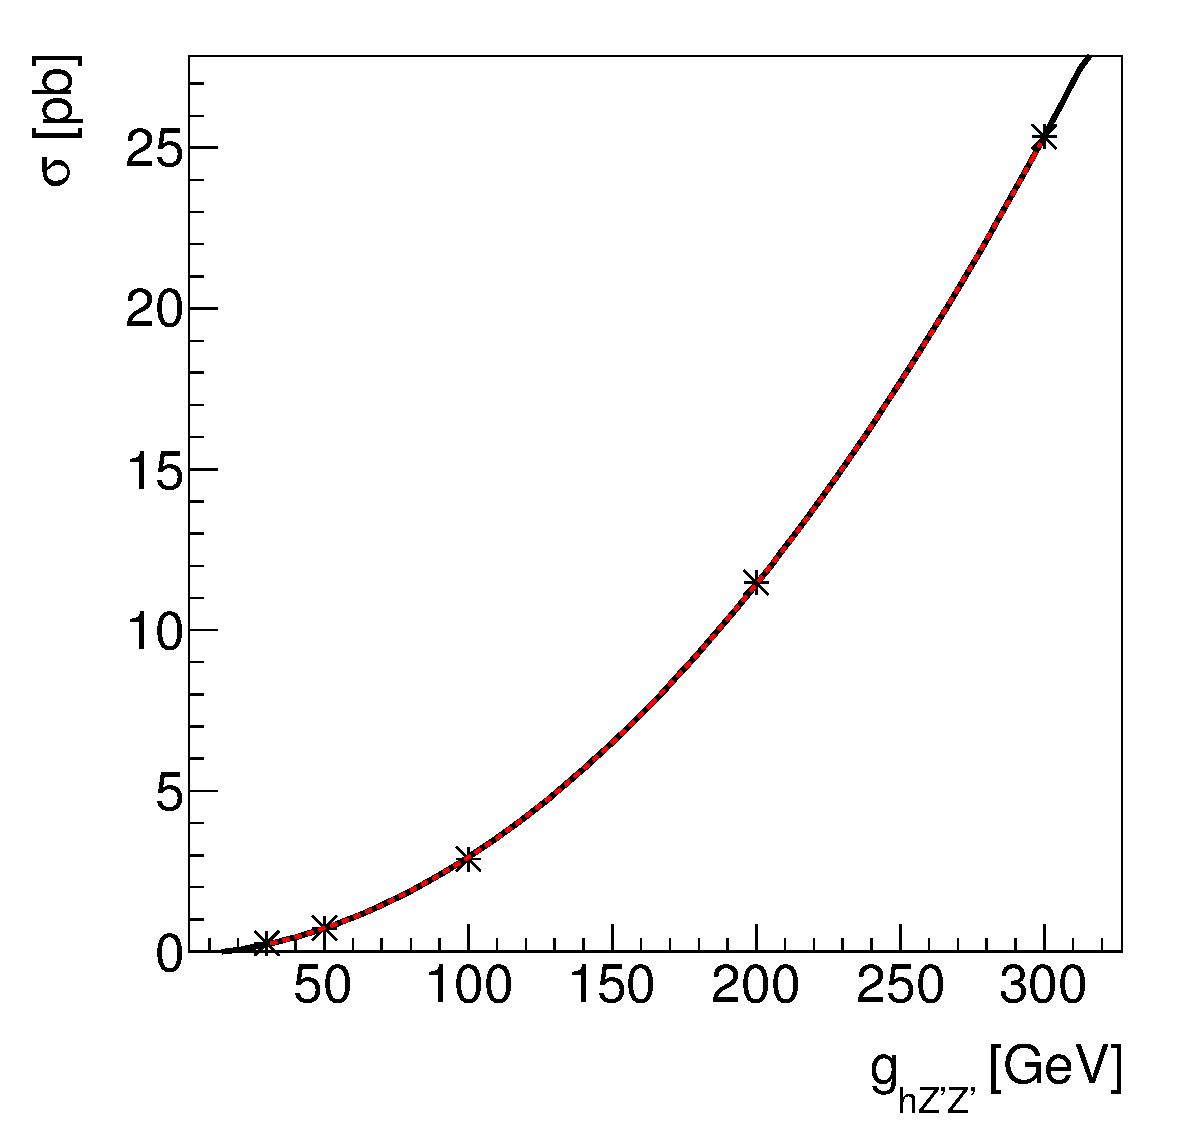
\includegraphics[width=0.49\linewidth]{figures/EW/monoH/zprime_xs_med_100}
	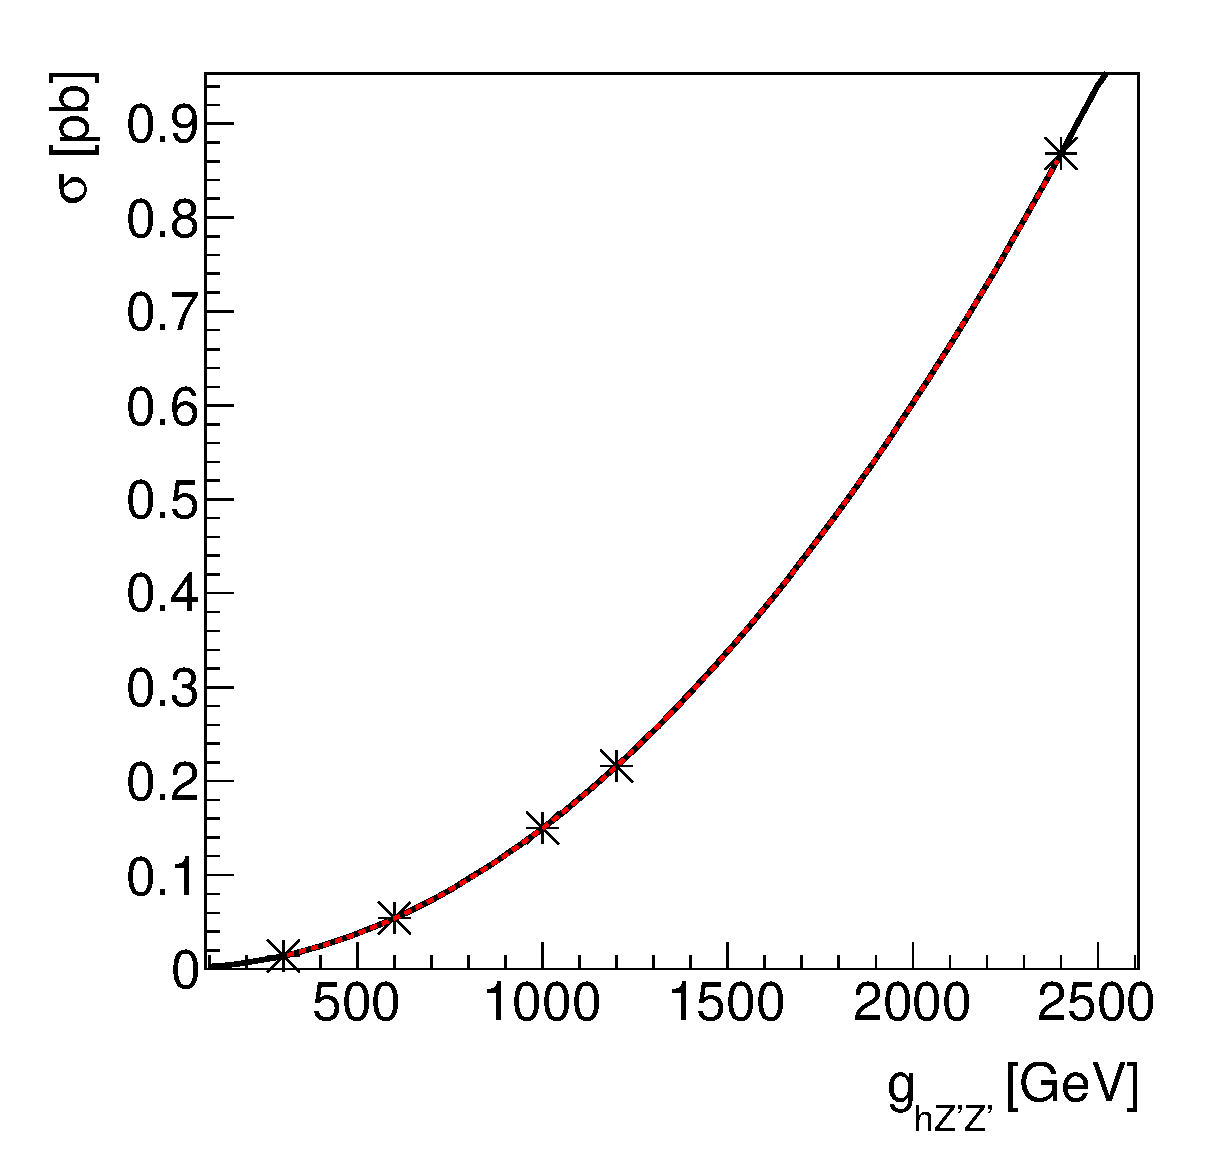
\includegraphics[width=0.49\linewidth]{figures/EW/monoH/zprime_xs_med_1000}
	\caption{Cross section of the $pp \rightarrow H\chiDM\bar{\chiDM}$ process as a function of 
		$g_{h \Zprime \Zprime}$ for $m_{\Zprime} = 100$~\gev (left) 
		and $m_{\Zprime} = 1$~\tev (right). The fit functions are shown in the text. 
		\label{fig:vectorXSdeps}}
\end{figure}

\clearpage

\subsection{\MET+Higgs from a scalar mediator}

A real scalar singlet $S$ coupling to DM can be introduced as a portal between SM and the dark sector 
through the Higgs field. The new scalar mixes with the SM Higgs boson, and couples to DM through a Yukawa term $y_\chiDM$. 
The relevant terms in the scalar potential are
\begin{align}
&V \supset a |H|^2 S + b |H|^2 S^2 + \lambda_h |H|^4 \notag \\
& \;\;\longrightarrow \tfrac{1}{2} a (h +  v)^2 S + \tfrac{1}{2}b (h +  v)^2 S^2 + \frac{\lambda_h}{4} (h +  v)^4 ,
\label{singlethiggsmix}
\end{align}
where $a,b$ are new physics couplings and $\lambda_h$ is the Higgs quartic.  

The additional Lagrangian terms for this model are: 
\be \label{LintScalar2}
L \supset - y_\chiDM \bar\chiDM \chiDM (  cos\theta\:S - sin\theta\: h ) - \frac{m_q}{v} \bar q q (cos\theta\: h + sin\theta\: S )  \,
\ee
where $\theta$ is the mixing angle between the Higgs boson and the new scalar. 

Mono-Higgs signals in this second model arise through processes shown in Fig.~\ref{fig:feyn_prod_monoH_S} (a,b), or through 
the radiation of a Higgs boson from the  $t$ quark in the production loop, in Fig.~\ref{fig:feyn_prod_monoH_S} (c). 
The first two processes depend on the $h^2 S$ and $h S^2$ cubic terms in Eq.~\eqref{singlethiggsmix}.  
At leading order in $\sin\theta$, these terms are
\be
V_{\rm cubic} \approx \frac{\sin\theta}{v} ( 2 m_h^2 + m_S^2) h^2 S  + b \, v \, h \, S^2 + ...
\ee
with $a$ and $\lambda_h$ expressed in terms of $\sin\theta$ and $m_h^2$, respectively.  
At leading order of $\sin\theta$, the $h^2 S$ term is fixed once the mass eigenvalues $m_h, m_S$ 
and mixing angle are specified.  The $h\,S^2$ term is not fixed and remains a free parameter of the model, depending on 
the new physics coupling $b$. 

\subsubsection{Parameter scan}

The model is described by five parameters: 

\begin{enumerate}
	\item the Yukawa coupling of heavy scalar to dark matter, \gDM (also referred to as $y_\chiDM$) 
	\item the mixing angle between heavy scalar and SM-like Higgs boson, $\sin\theta$;
	\item the new physics coupling, $b$;
	\item mass of heavy scalar, $m_{S}$, also termed \mmed;
	\item mass of dark matter, \mDM;
	%(also referred to as $m_{\chiDM}$)
\end{enumerate}

The mixing angle is constrained from current Higgs data
to satisfy $\cos\theta = 1$ within 10\% and therefore $\sin\theta \lesssim 0.4$. This provides a starting point 
for the parameter scan in this model: we recommend to set $\sin\theta = 0.3$. 
Figure~\ref{fig:metScalarCoupling2} shows that
there is no dependence of the kinematics from the value of this angle, and different values can be obtained via rescaling
the results for this mixing angle according to the relevant cross-section. It can also be observed from Figures~\ref{fig:metScalarMass} and~\ref{fig:metScalarCoupling} 
that the kinematics of this model follows that of the equivalent jet+\MET model: only small changes are observed
in the on-shell region, while the relevant distributions diverge when the mediator is off-shell. 
For this reason, the same grid in \mmed, \mdm as for the scalar mediator
of the jet+\MET search (Table~\ref{tab:mDMmMedScan_SP}) is chosen as a starting point. \Todo{Estimate the sensitivity and possibly prune parameter scan.}
The Yukawa coupling to DM $y_{DM}$ is set to 1, the 
new physics coupling between scalar and SM Higgs $b$ = 3. Results for other values can be obtained via a 
rescaling of the results for these parameters. 
%More detailed studies are required to estimate the reach of the analysis with respect to all points in the grid
%and therefore decide on a smaller set of grid points to be generated; 
%those are left to the individual analyses. 

\begin{figure}[hbpt!]
	\begin{center}
		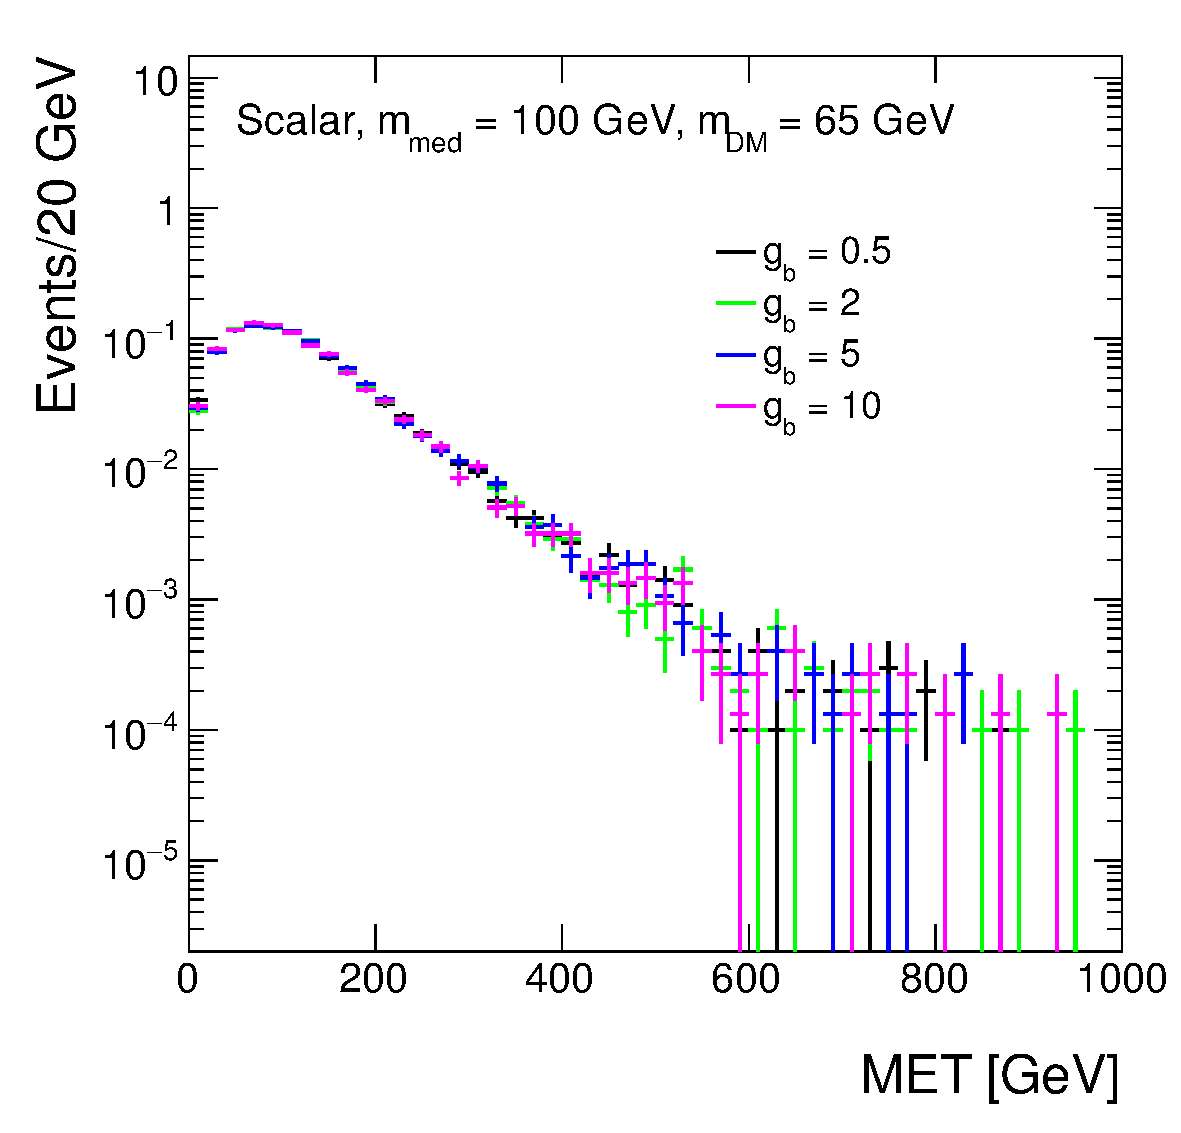
\includegraphics[width=0.49\linewidth]{figures/EW/monoH/s_gb_65_100_04_MET_et_Log}
		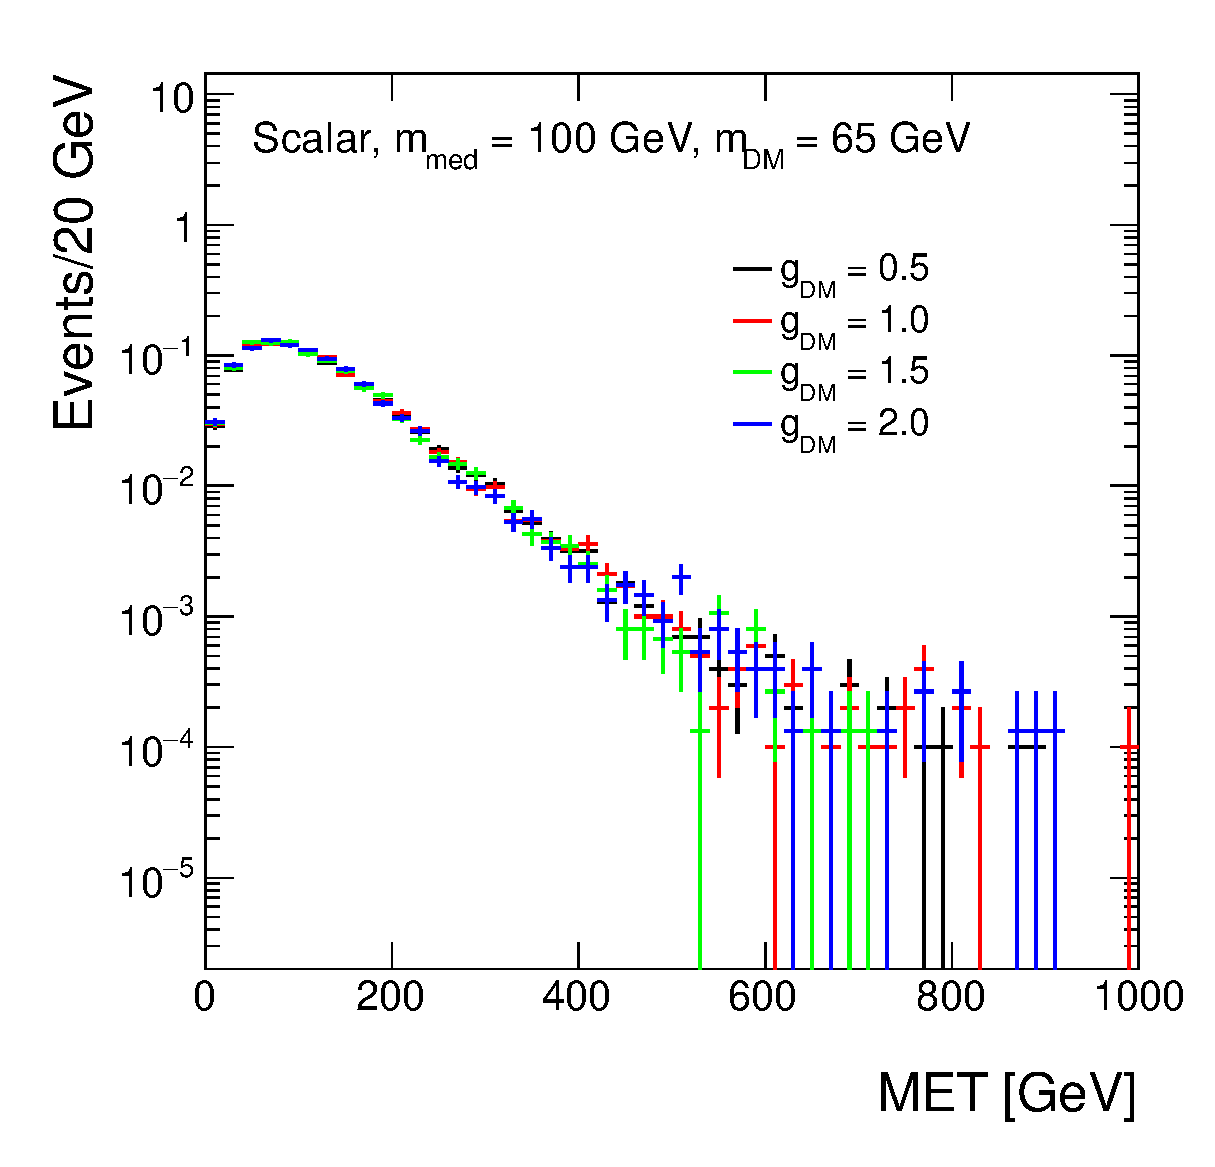
\includegraphics[width=0.49\linewidth]{figures/EW/monoH/s_gdm_MET_et_Log}
		\caption{Missing transverse momentum distributions at generator level in the scalar 
			mediator scenario, for different values of: the new physics coupling $g_b$ (left),
			and the mediator-dark matter coupling \gDM (right).
			\label{fig:metScalarCoupling}}
	\end{center}
\end{figure}

\begin{figure}[hbpt!]
	\begin{center}
		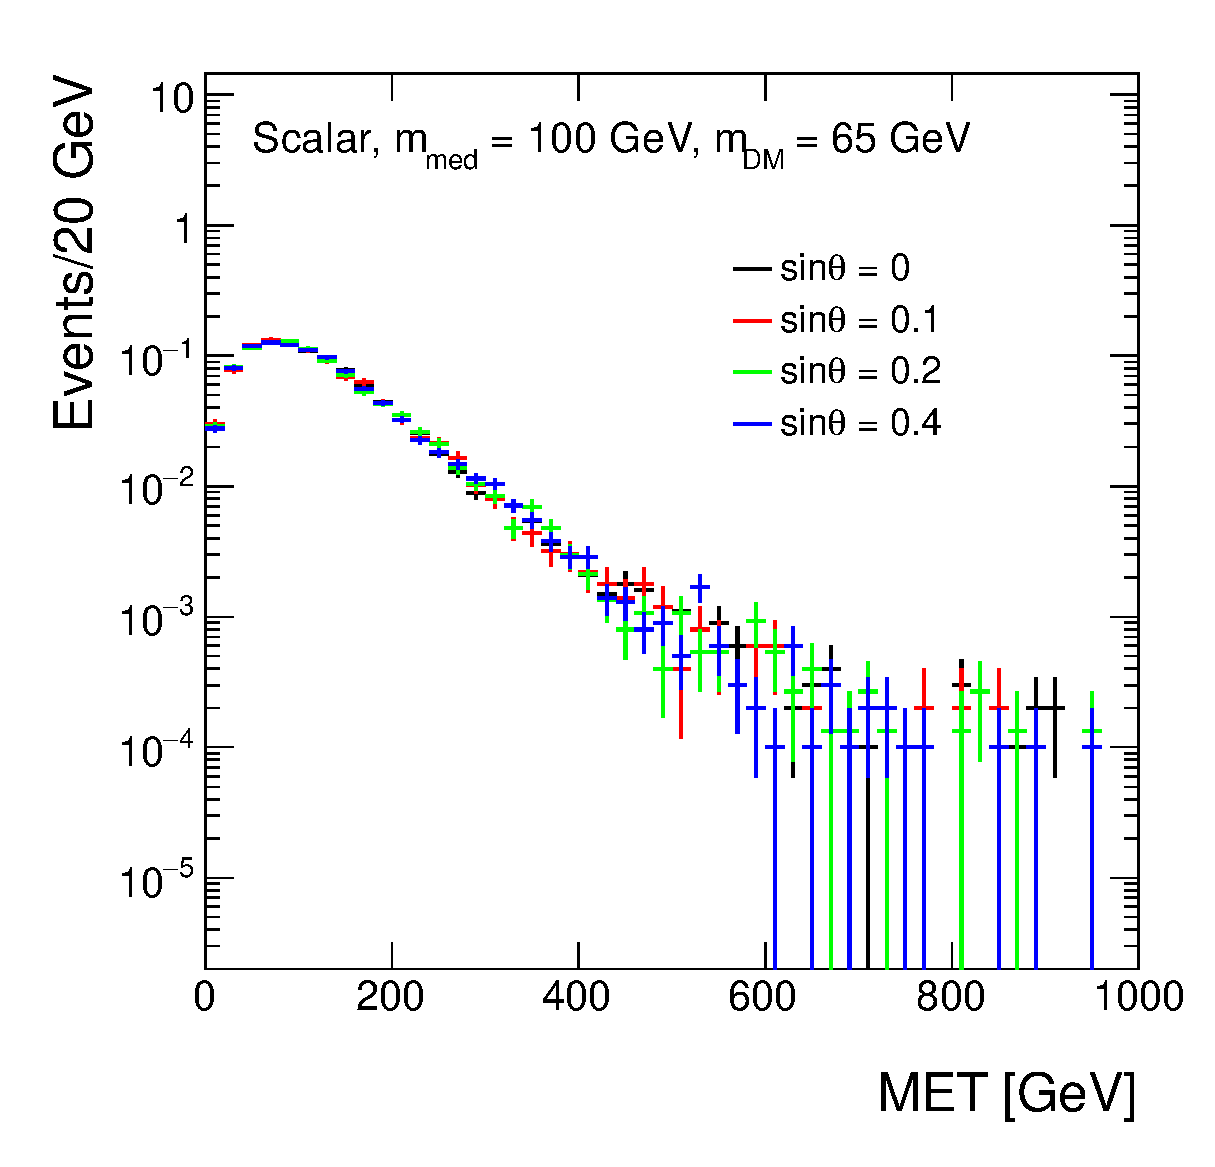
\includegraphics[width=0.49\linewidth]{figures/EW/monoH/s_theta_65_100_2_MET_et_Log}
		\caption{Missing transverse momentum distributions at generator level in the scalar 
			mediator scenario: for different values of the mixing angle $\sin\theta$.
			\label{fig:metScalarCoupling2} }
	\end{center}
\end{figure}

\begin{figure}[hbpt!]
	\begin{center}
		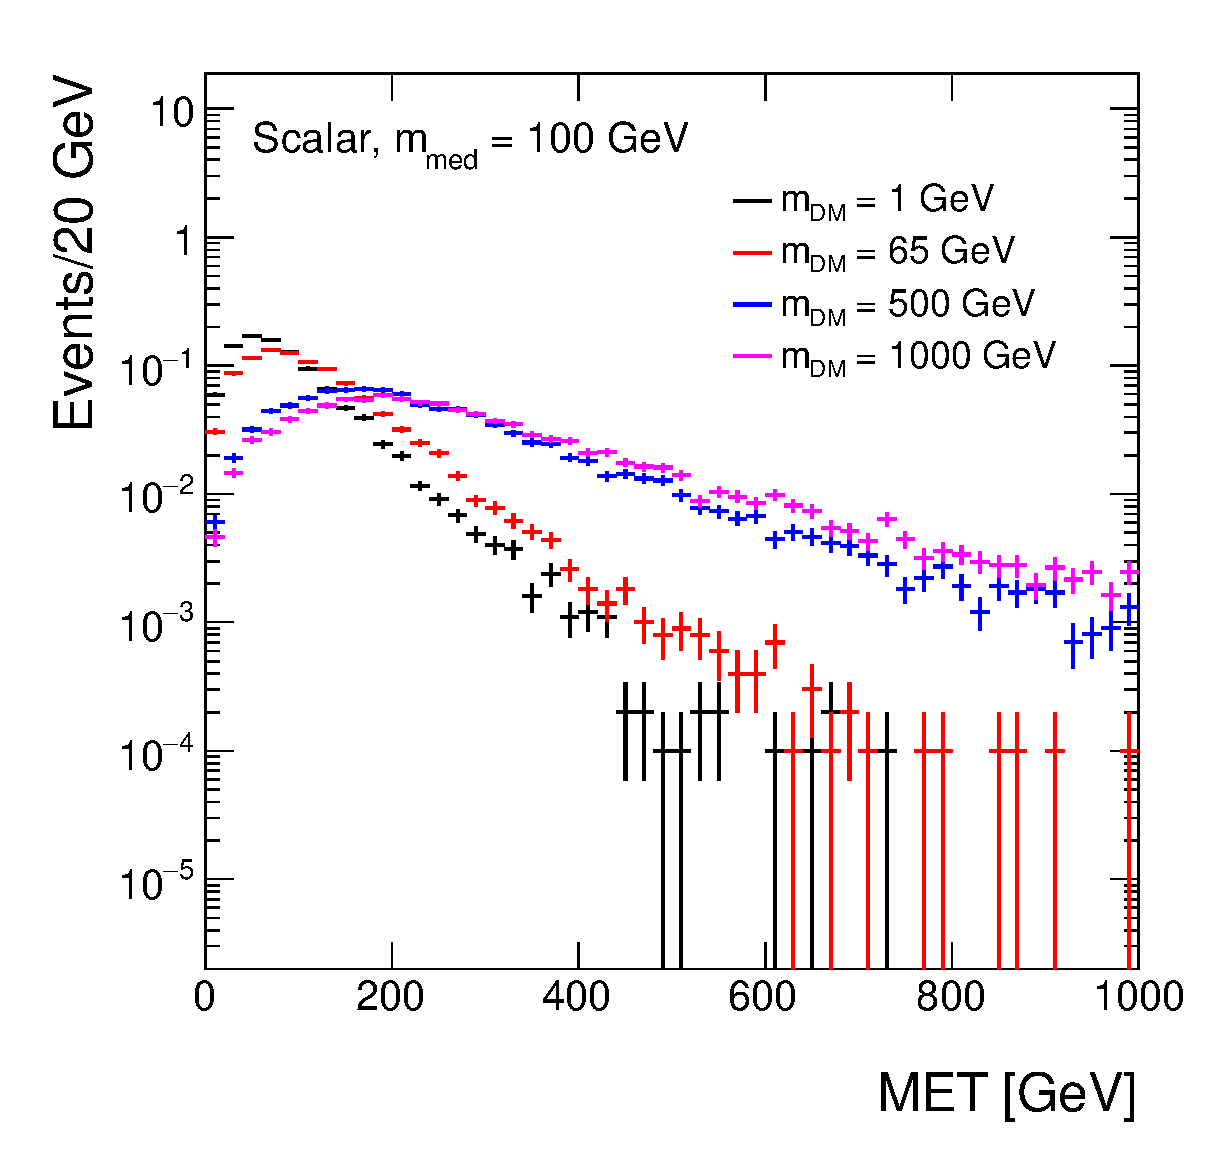
\includegraphics[width=0.49\linewidth]{figures/EW/monoH/scalar_100_MET_et_Log}
		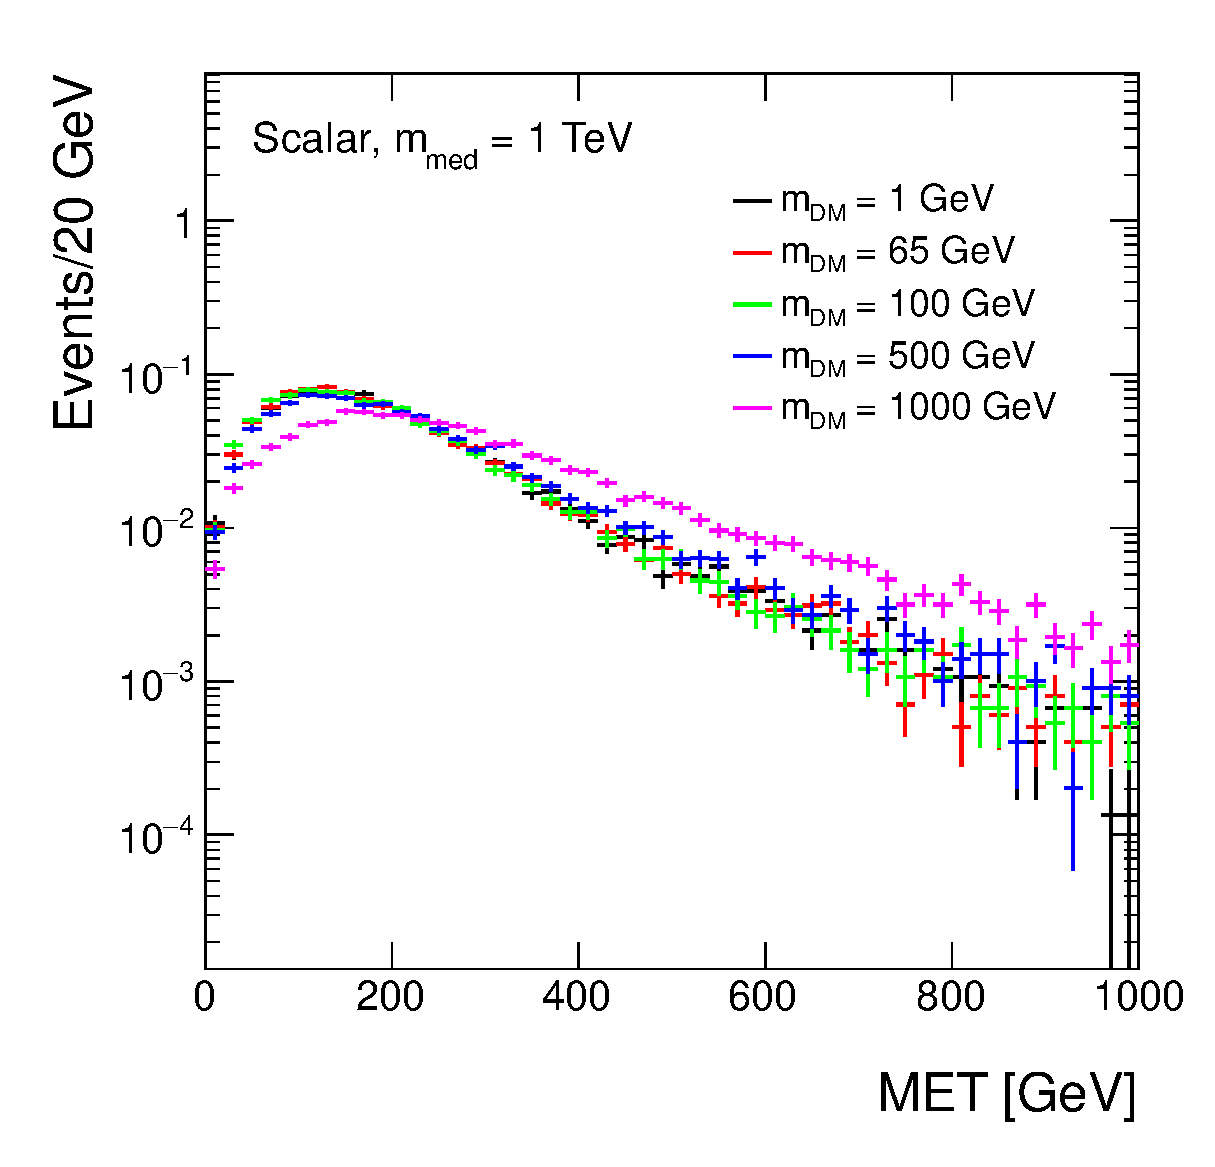
\includegraphics[width=0.49\linewidth]{figures/EW/monoH/scalar_1000_MET_et_Log}
		\caption{Missing transverse momentum distributions at generator level in the scalar 
			mediator scenario: for different values of the dark matter mass \mDM 
			and a mediator mass of $\mMed = 100~\gev$ (left) and $\mMed = 1~\tev$ (right).
			\label{fig:metScalarMass}}
	\end{center}
\end{figure}

Figs. ~\ref{fig:ScalarHbb_100} and ~\ref{fig:ScalarHbb_1000} show the kinematic distributions for the two leading jets
in the $H \to \bar b b$ decay channel, for two values of the mediator mass and varying the DM mass.  

\begin{figure}[hbpt!]
	\centering
	\subfloat[Leading $b-$jet transverse momentum]{
		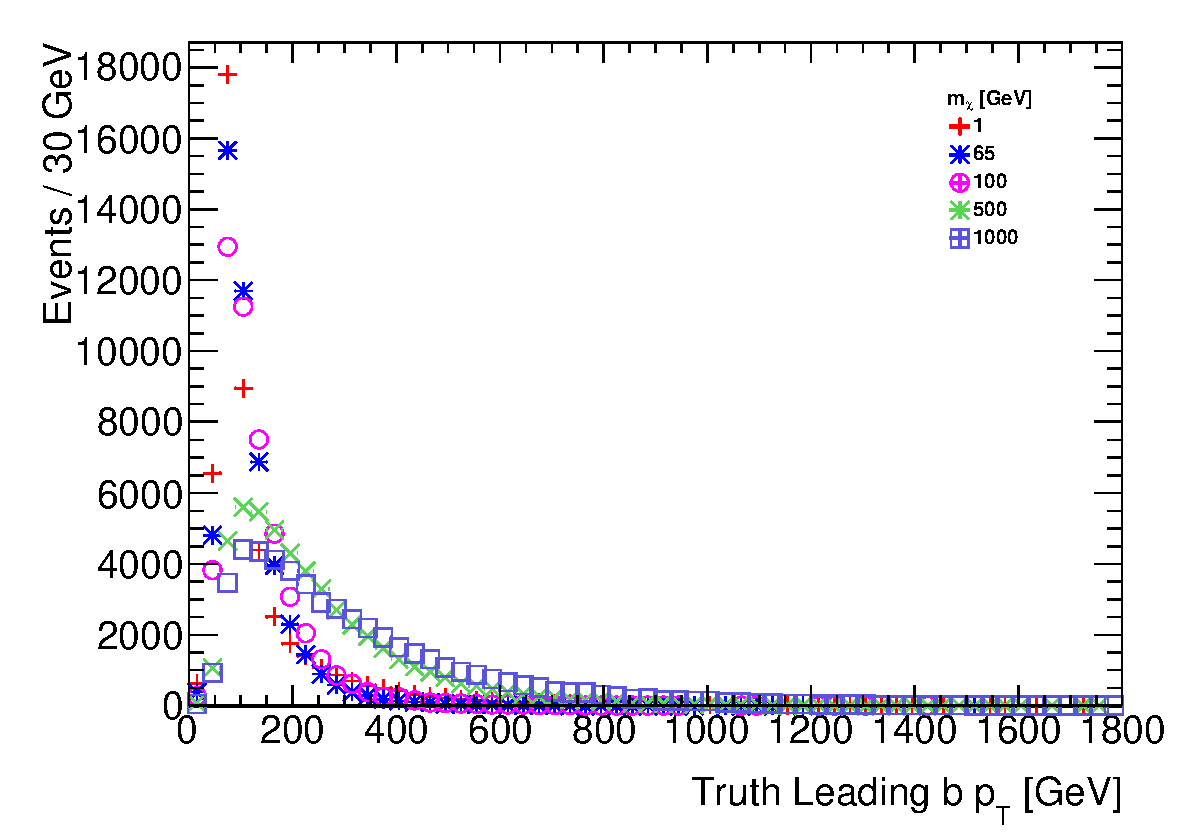
\includegraphics[width=0.47\linewidth]{figures/EW/monoH/scalar100/truth_leading_b_pt} %\label{fig:met_cmp_high}
	}
	\hfill
	\subfloat[Leading $b-$jet pseudorapidity]{
		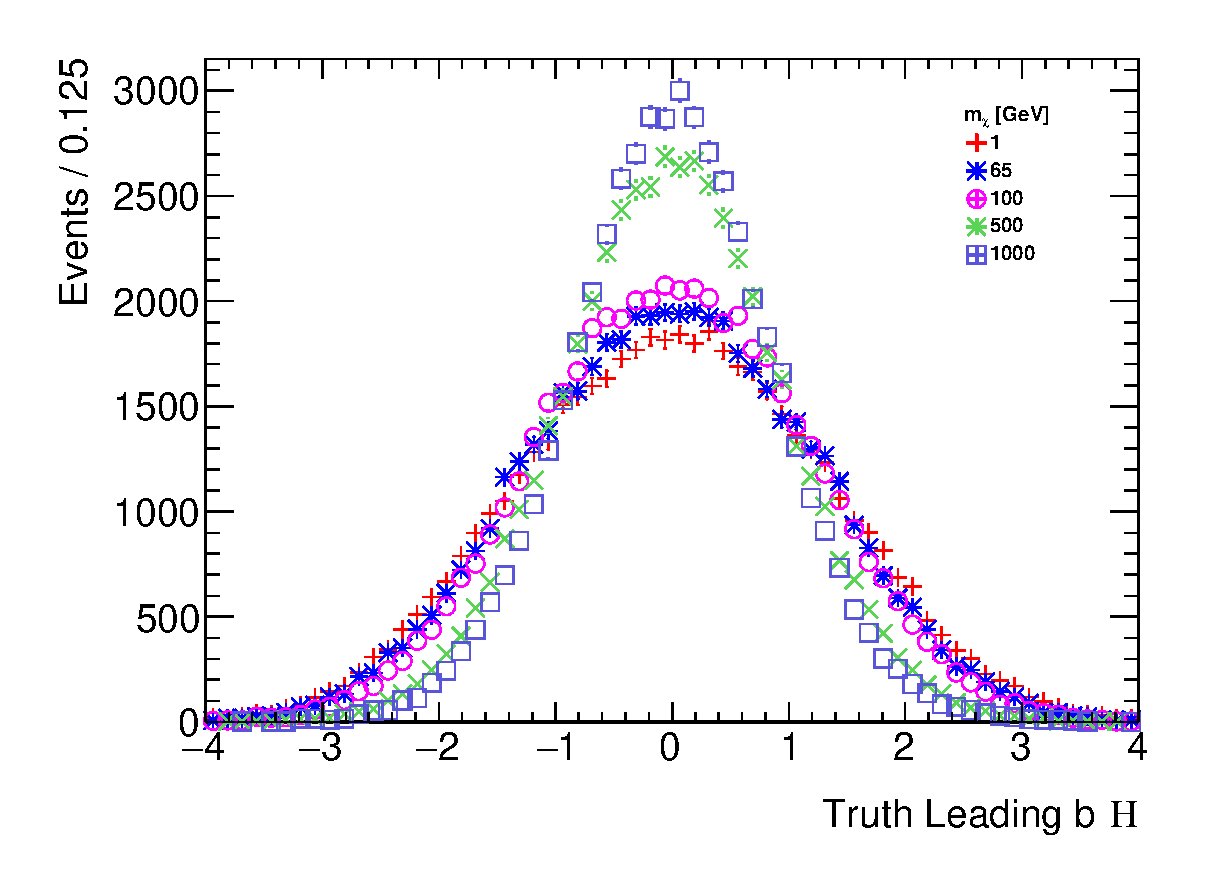
\includegraphics[width=0.47\linewidth]{figures/EW/monoH/scalar100/truth_leading_b_eta} %\label{fig:met_cmp_low}
	}
%	\hfill
%	\subfloat[Leading $b-$jet transverse momentum]{
%		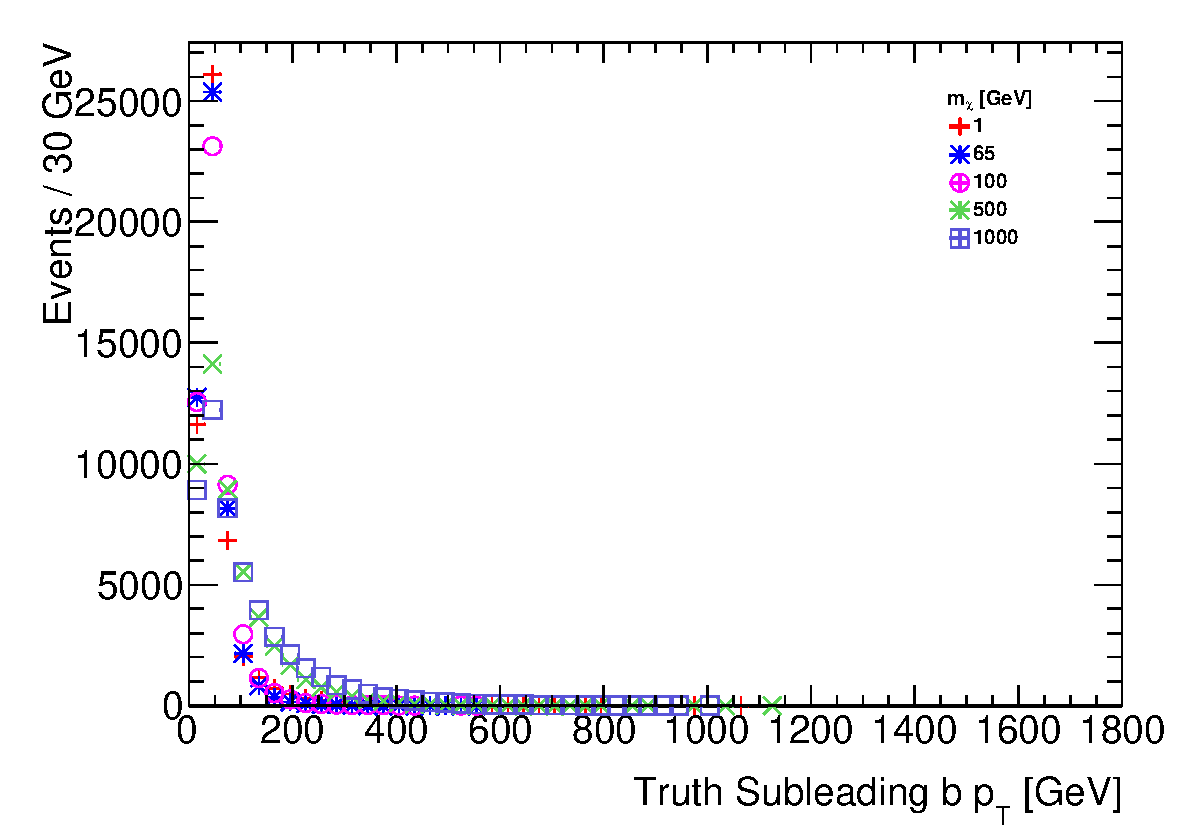
\includegraphics[width=0.47\linewidth]{figures/EW/monoH/scalar100/truth_subleading_b_pt} %\label{fig:met_cmp_high}
%	}
%	\hfill
%	\subfloat[Leading $b-$jet pseudorapidity]{
%		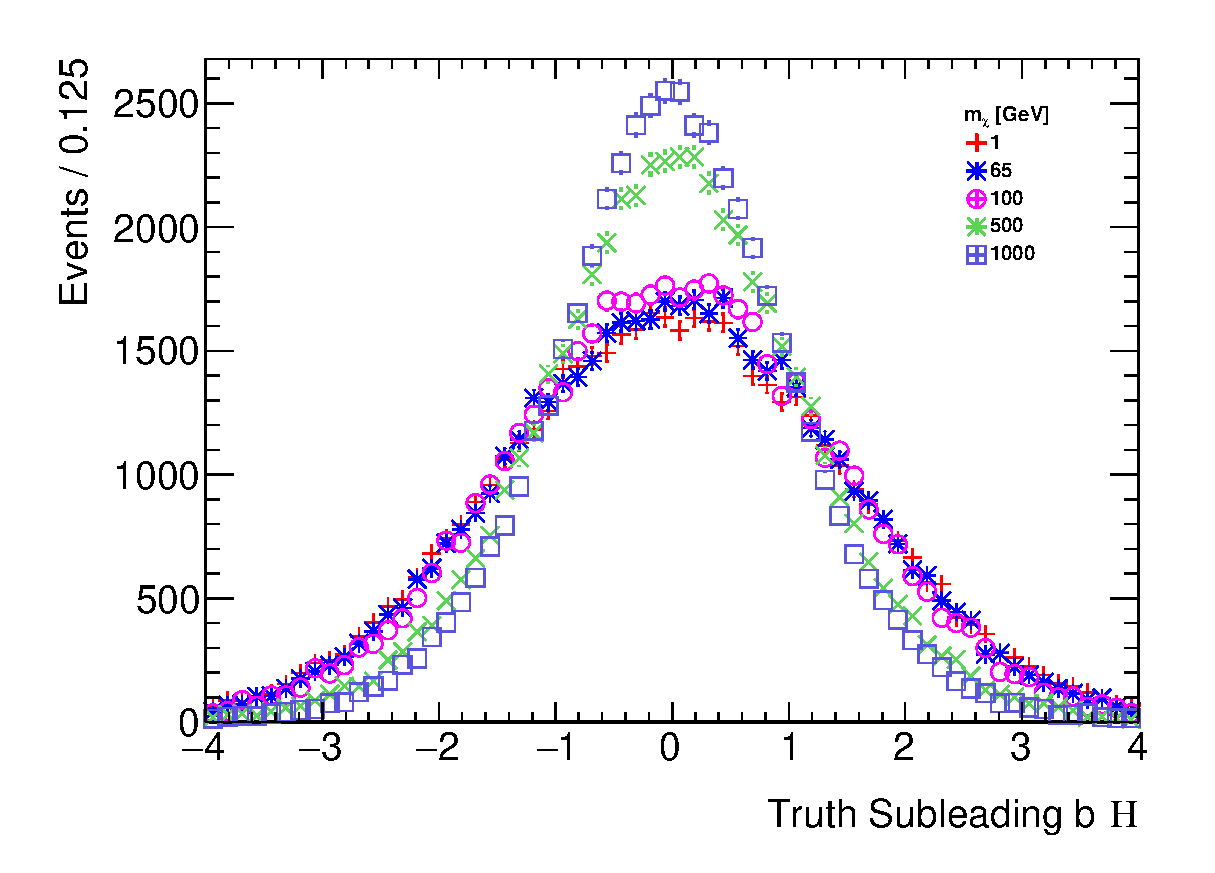
\includegraphics[width=0.47\linewidth]{figures/EW/monoH/scalar100/truth_subleading_b_eta} %\label{fig:met_cmp_low}
%	}
	\hfill
	\subfloat[Angular distance between the two leading $b-$jets]{
		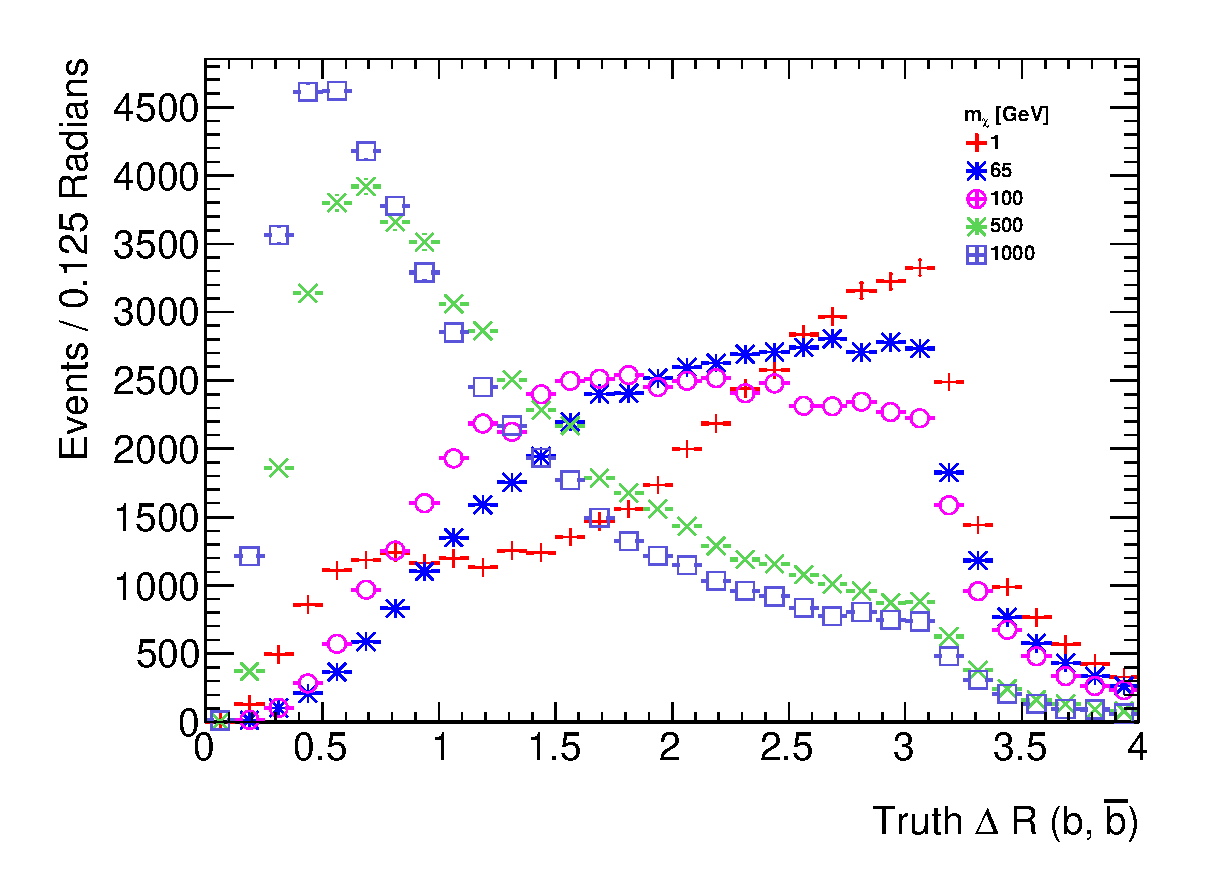
\includegraphics[width=0.47\linewidth]{figures/EW/monoH/scalar100/truth_bb_deltar} %\label{fig:met_cmp_low}
	}

	\caption{Comparison of the kinematic distributions for the two leading jets from the Higgs decay in the scalar simplified model, 
		when fixing the new scalar mass to 100~\gev and varying the DM mass. 
		\label{fig:ScalarHbb_100}}
\end{figure}

\begin{figure}[hbpt!]
	\centering
	\subfloat[Leading $b-$jet transverse momentum]{
		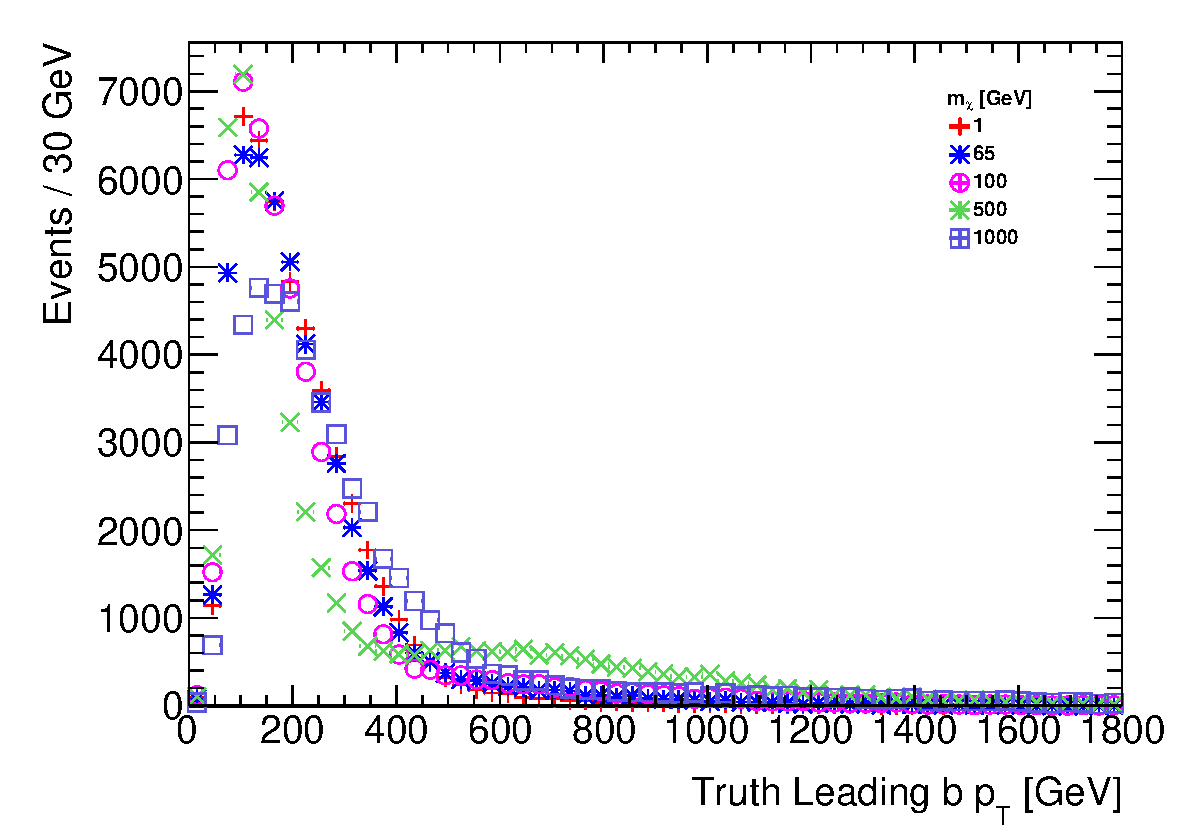
\includegraphics[width=0.47\linewidth]{figures/EW/monoH/scalar1000/truth_leading_b_pt} %\label{fig:met_cmp_high}
	}
	\hfill
	\subfloat[Leading $b-$jet pseudorapidity]{
		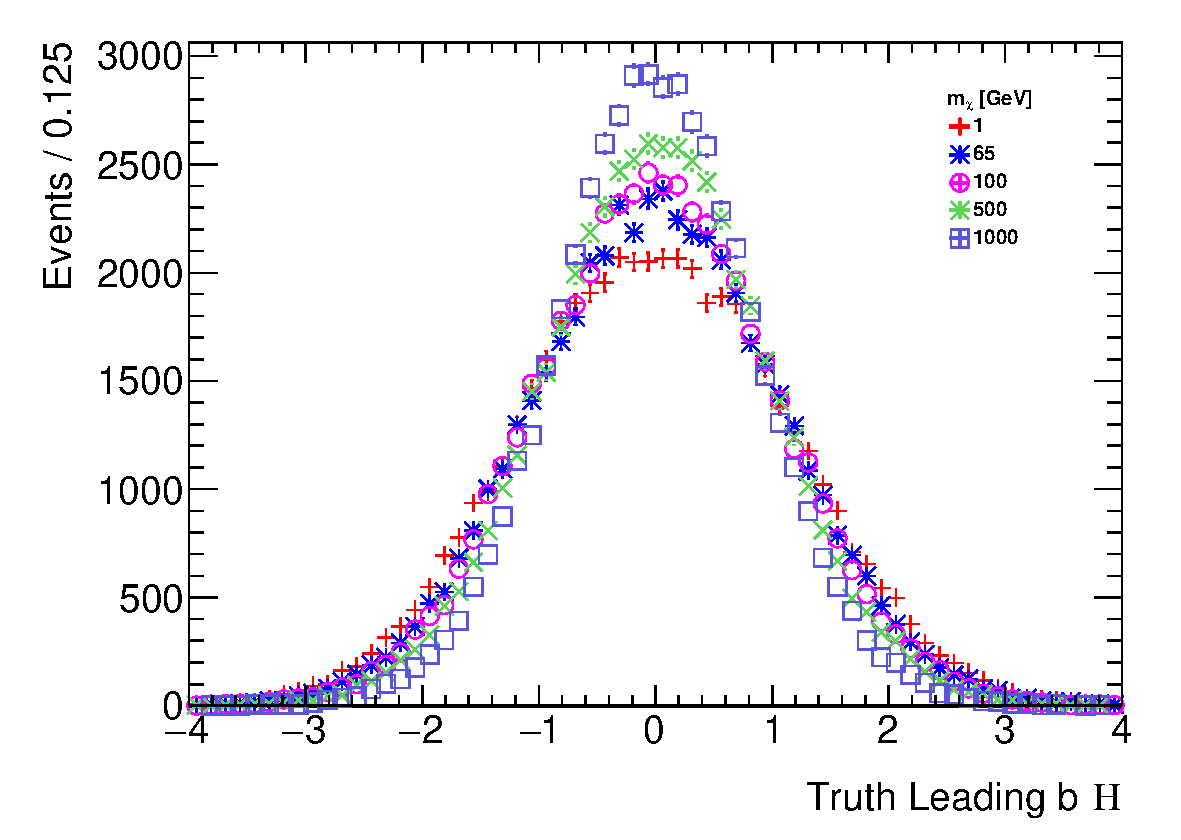
\includegraphics[width=0.47\linewidth]{figures/EW/monoH/scalar1000/truth_leading_b_eta} %\label{fig:met_cmp_low}
	}
%	\hfill
%	\subfloat[Leading $b-$jet transverse momentum]{
%		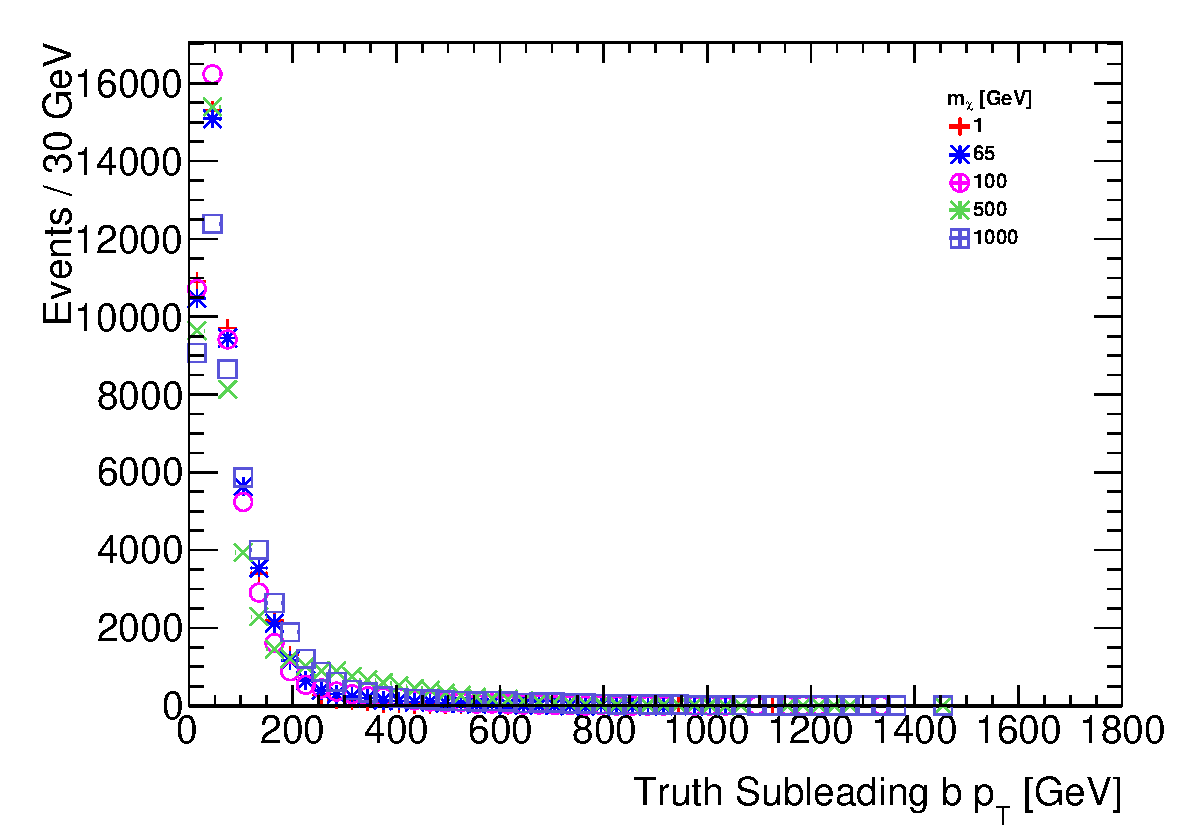
\includegraphics[width=0.47\linewidth]{figures/EW/monoH/scalar1000/truth_subleading_b_pt} %\label{fig:met_cmp_high}
%	}
%	\hfill
%	\subfloat[Leading $b-$jet pseudorapidity]{
%		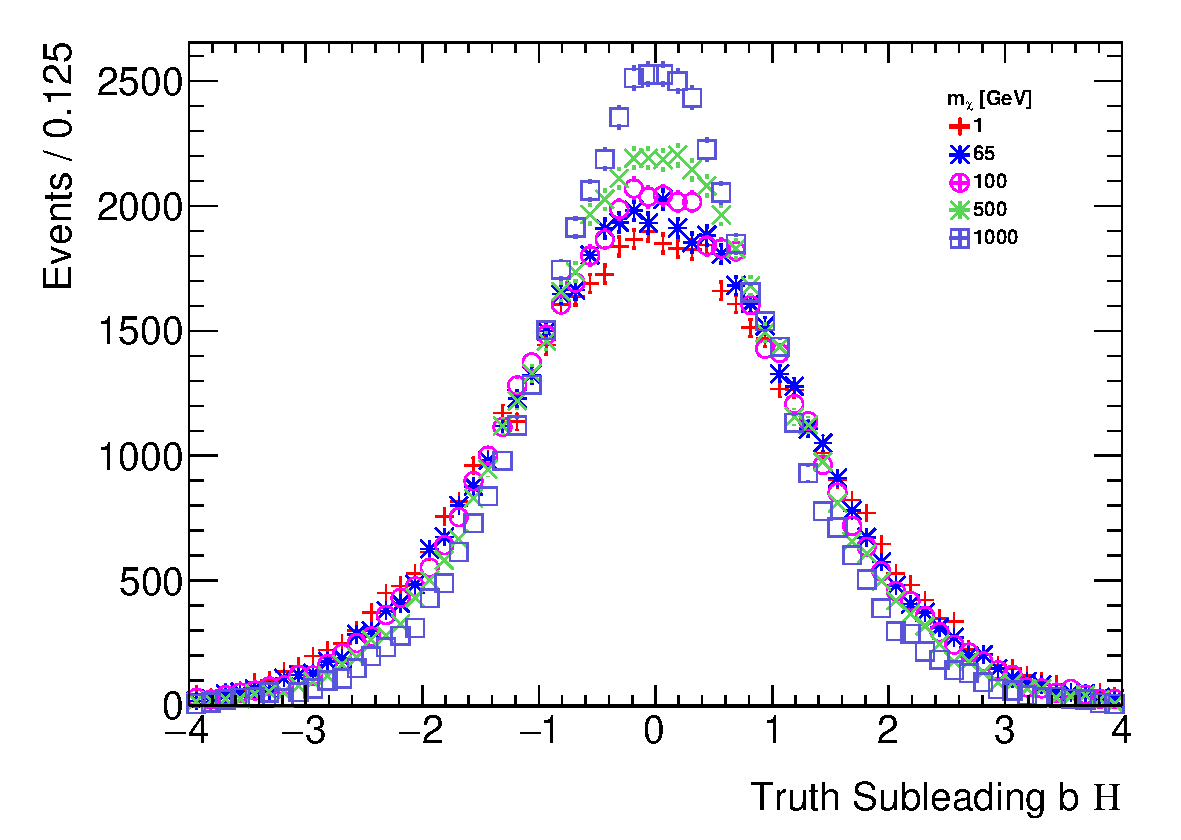
\includegraphics[width=0.47\linewidth]{figures/EW/monoH/scalar1000/truth_subleading_b_eta} %\label{fig:met_cmp_low}
%	}
	\hfill
	\subfloat[Angular distance between the two leading $b-$jets]{
		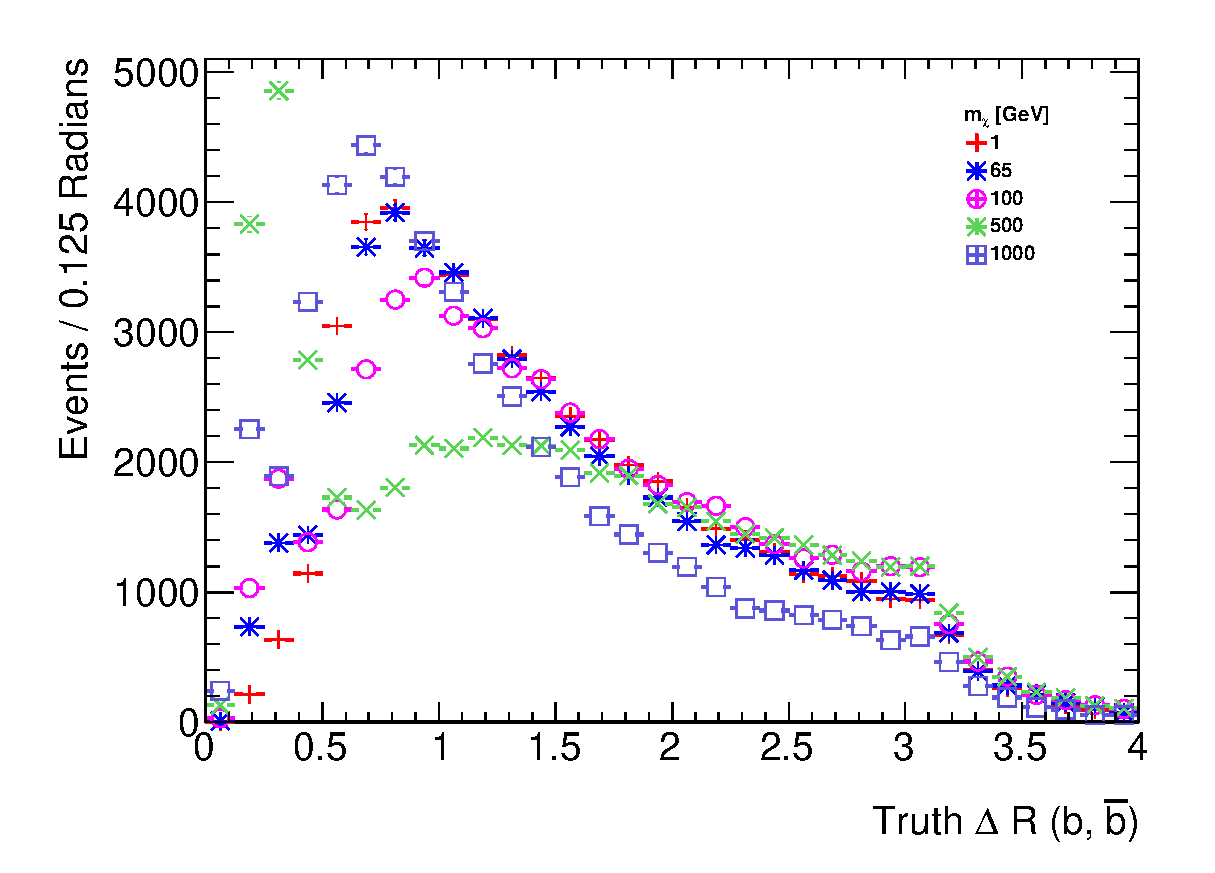
\includegraphics[width=0.47\linewidth]{figures/EW/monoH/scalar1000/truth_bb_deltar} %\label{fig:met_cmp_low}
	}
	\caption{Comparison of the kinematic distributions for the two leading jets from the Higgs decay in the scalar simplified model, 
		when fixing the new scalar mass to 1000~\gev and varying the DM mass. 
		\label{fig:ScalarHbb_1000}}
\end{figure}


%%%
\subsection{Higgs+\MET signal from 2HDM model with a \Zprime and a new pseudoscalar}

In this simplified model~\cite{Berlin:2014cfa}, a new \Zprime resonance decays to a Higgs boson $h$ 
plus a heavy pseudoscalar state 
$A^0$ in the 2HDM framework, which in turn decays to a DM pair. This model is 
represented in the diagram in Fig. \ref{fig:feyn_prod_monoH} (b).


The motivation for coupling the dark matter to the pseudoscalar is that dark matter coupling to a Higgs or \Zprime boson is generically 
constrained by other signal channels and direct detection. 
An advantage of including this model is that it has different kinematics  due to the on-shell \Zprime production, 
where for heavy \Zprime masses the \MET and pT spectra are much harder.
This model can satisfy electroweak precision tests and constraints from dijet resonance searches, 
and still give a potentially observable Higgs+\MET signal.
 
 This model comprises two doublets, where $\Phi_u$ couples to up-type quarks and $\Phi_d$ couples to down-type
 quarks and leptons:
 \begin{equation}
 -{\cal L} \supset  y_u Q \tilde \Phi_u \bar u + y_d Q \Phi_d \bar d + y_e L \Phi_d \bar e  + {\rm h.c.}
 \end{equation}
 
 After electroweak symmetry breaking, the Higgs doublets attain vacuum expectation values $v_u$ and $v_d$, and in unitary gauge the doublets are parametrized as
 \begin{align}
 \Phi_d &= \frac{1}{\sqrt{2}}
 \begin{pmatrix}
 -\sin{\beta} \ H^+ \\ v_d - \sin{\alpha} \ h + \cos{\alpha} \ H - i \sin{\beta} \ A^0
 \end{pmatrix} 
 \quad , \nonumber \\
 \Phi_u &= \frac{1}{\sqrt{2}}
 \begin{pmatrix}
 \cos{\beta} \ H^+ \\ v_u + \cos{\alpha} \ h + \sin{\alpha} \ H + i \cos{\beta} \ A^0
 \end{pmatrix}
 \end{align}
 where $h,H$ are neutral CP-even scalars and $A^0$ is a neutral CP-odd scalar. 
 In this framework, $\tan{\beta} \equiv v_u/v_d$, and $\alpha$ is the mixing angle that diagonalizes 
 the $h - H$ mass squared matrix. 
 %FIXME: this is an external constrain that may or may not be included 
%The masses of the remaining scalars $H, A^0, H^\pm$ are assumed to be 
%around or above $300$~\gev, respecting $b \to s \gamma$ constraints \cite{Branco:2011iw}.
We take $\alpha = \beta - \pi/2$, in the 
%alignment 
limit where $h$ has SM-like couplings to fermions and 
gauge bosons as per Ref.~\cite{Craig:2013hca}, and $\tan{\beta} \ge 0.3$ 
as implied from the perturbativity of the top Yukawa coupling. 
  %For the $ b \bar{b}$ decay channel, the signature of the signal we are searching for is a pair of boosted WIMPs recoiling against two $b$ jets. 
The Higgs vacuum expectation values lead to $Z-\Zprime$ mass mixing, with a mixing parameter given by 
 \begin{align}
 \epsilon & \equiv \frac{1}{M_{\Zprime}^2 - M_Z^2} \frac{g g_z}{2 \cos{\theta_w}} ( z_d v_d^2 + z_u v_u^2) \nonumber \\
 & =  \frac{(M_Z^0)^2}{M_{\Zprime}^2 - M_Z^2} \frac{2 g_z \cos \theta_w}{g}  z_u \sin^2 \beta.
 \label{eq:epsilon}
 \quad
 \end{align}
  
The production cross section for this model scales as $(g_z)^2$, as the decay width for this process
to leading order in $\epsilon$ (Eq.~\ref{eq:epsilon}) is
\begin{equation}
\Gamma_{\Zprime \to h A^0} =  (g_z \cos \alpha \cos \beta)^2 \frac{|p|}{24 \pi} \frac{|p|^2}{M_{\Zprime}^2}.
\end{equation}
where the center of mass momentum for the decay products $|p| =
\frac{1}{2 M_{\Zprime}} \lambda^{1/2}(M_{\Zprime}^2,m_h^2, m_{A^0}^2)$, and
$\lambda$ is the K\"{a}llen triangle function\sidenote{\vskip -2.5\baselineskip\begin{align*}\lambda(c_1,c_2,c_3) \equiv&\;c_1^2 + c_2^2 + c_3^2\\ 
						&- 2(c_1 c_2 + c_2 c_3 + c_3 c_1)\end{align*}}.
   
%  Diagonalizing the gauge
% boson mass matrix, the tree-level masses of the $Z$ and \Zprime bosons are given by
% \begin{align}
% M_Z^2 &\approx ( M_{Z}^0)^2  - \epsilon^2 \left[( M_{\Zprime}^0)^2 - ( M_{Z}^0)^2 \right] \nonumber \\
% M_{\Zprime}^2 &\approx ( M_{\Zprime}^0)^2 + \epsilon^2 \left[( M_{\Zprime}^0)^2 - ( M_{Z}^0)^2 \right]
% \quad ,
% \label{eq:Zpmasses}
% \end{align}
% where $(M_Z^0)^2 = g^2(v_d^2+ v_u^2)/(4\cos^2{\theta_w}) $ and
% $(M_{\Zprime}^0)^2 = g_z^2 ( z_d^2 v_d^2 + z_u^2 v_u^2 + z_\phi^2
% v_\phi^2)$ are the mass-squared values in the absence of mixing. The
% result above is accurate to order $\epsilon^2$, where $\epsilon$ is
% a small mixing parameter given by
% \begin{align}
% \epsilon & \equiv \frac{1}{M_{\Zprime}^2 - M_Z^2} \frac{g g_z}{2 \cos{\theta_w}} ( z_d v_d^2 + z_u v_u^2) \nonumber \\
% & =  \frac{(M_Z^0)^2}{M_{\Zprime}^2 - M_Z^2} \frac{2 g_z \cos \theta_w}{g}  z_u \sin^2 \beta.
% \label{eq:epsilon}
% \quad
% \end{align}
 
\subsubsection{Parameter scan}
 
 The model is described by five parameters:
 \begin{itemize}
 	\item the pseudoscalar mass $M_{A^0}$,
 	\item the DM mass \mDM,
 	\item the \Zprime mass, $M_{\Zprime}$,
    \item $\tan{\beta} (\equiv v_u/v_d)$,
 	\item the \Zprime coupling strength $g_z$. 
 \end{itemize}

 To study the signal production and kinematic dependencies on these parameters, 
 we produced signal samples varying each of the five parameters through 
 MadGraph for the matrix element, PYTHIA for the parton shower, and DELPHES\cite{deFavereau:2013fsa} 
for a parameterized detector-level simulation.
 
 As seen in Fig.~\ref{fig:DMH_tanbeta}, variations of $\tan{\beta}$ does not lead to any kinematic 
 difference and the production cross section simply scales as a function of $\tan{\beta}$. Hence 
we recommend to fix $\tan{\beta}$ to unity in the signal generation. 


\begin{figure}[h!]
\centering
\subfloat[\MET distribution]{
	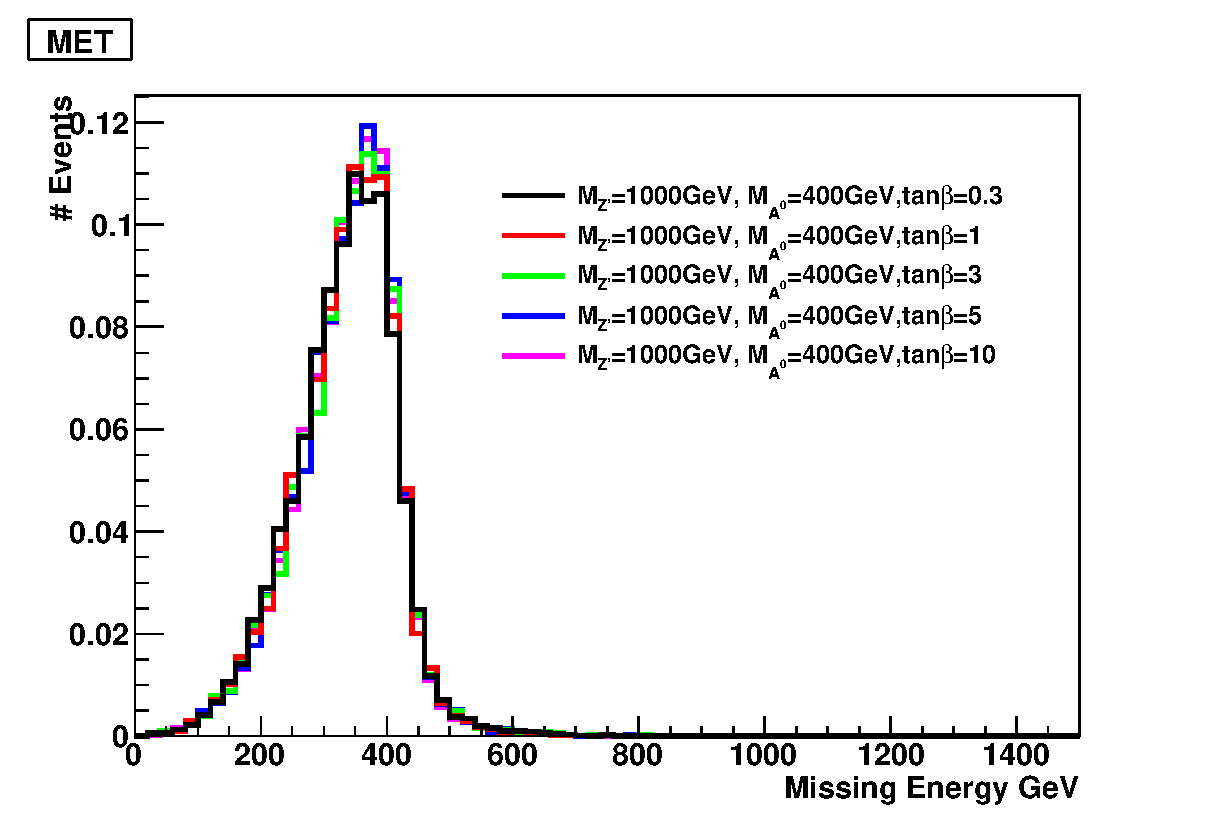
\includegraphics[width=0.47\linewidth]{figures/EW/monoH/2hdm/hxx_zp1000dm10gz01_met}
}
\hfill
\subfloat[$\Delta\phi$ distance between the two $b-$ jets]{
	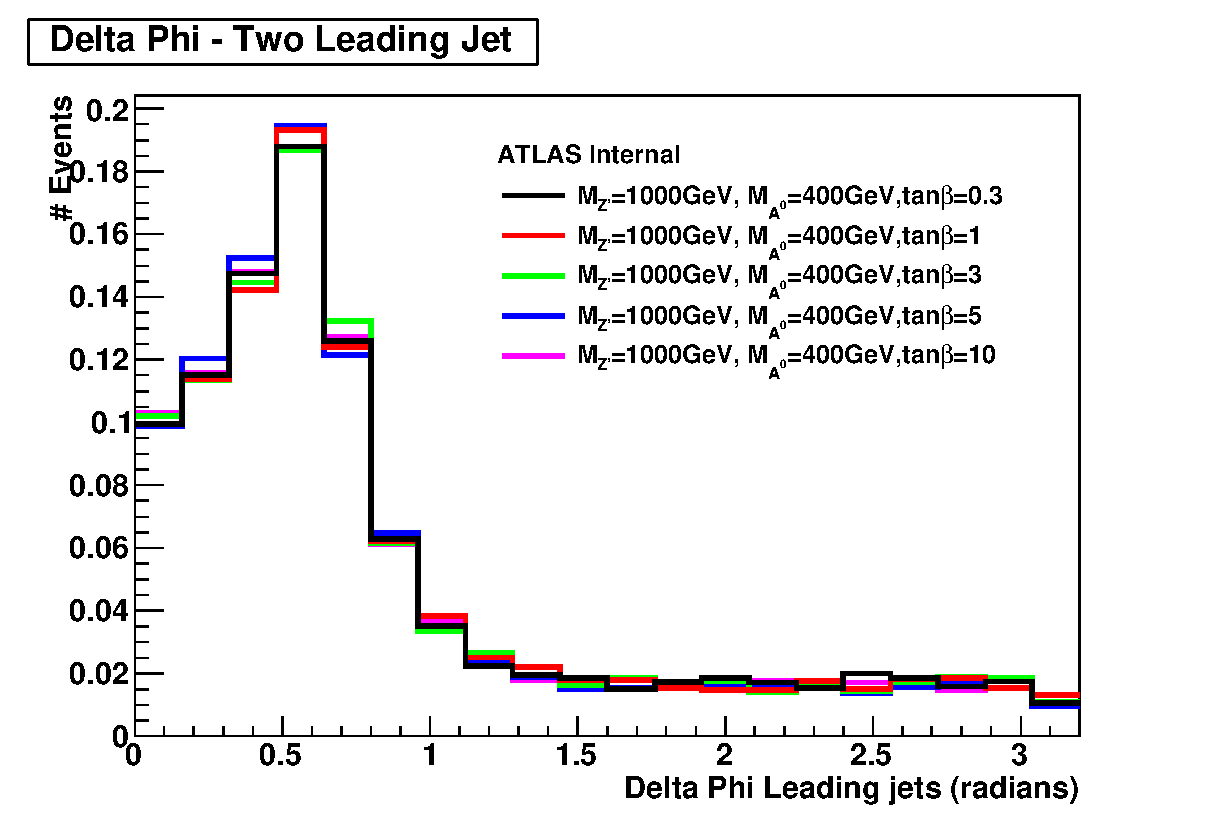
\includegraphics[width=0.47\linewidth]{figures/EW/monoH/2hdm/hxx_zp1000dm10gz01_dphi12}
}
\caption{Kinematic distributions of the signal process varying $\tan{\beta}$, in the case of a Higgs boson decaying into two $b$ quarks,
	after parameterized detector simulation: no kinematic dependency is observed}
\label{fig:DMH_tanbeta}
\end{figure}

Similarly, variations of $g_z$ do not lead to any kinematic changes. 
The value of $g_z$ for a given $M_{\Zprime}$ and $\tan \beta$ can be set according to the maximum value allowed by electroweak global 
fits and dijet constraints, as described in~\cite{Berlin:2014cfa}. Since this parameter does not influence the kinematics, 
we leave it up to individual analyses on whether they generate benchmark points only according to these external constraints.
%\textbf{[TODO: add link to section as in summary. This is the same sentence we will put in for the mono-b model]}.   
%For \Zprime masses below $\sim 1.3$~\tev and larger $\tan \beta$, the $\rho_0$ constraint on $g_z$ is stronger than 
%dijet limits, while for $\tan \beta \lesssim 0.6$,
%the dijet constraints dominate even at low \Zprime masses. 

Since the DM pair are produced as a result of the decay of $A^0$, there are minimal kinematic changes when varying \mDM
as long as $\mDM<M_{A^0}/2$ so that $A^0$ production is on-shell, as shown in Fig.~\ref{fig:DMH_mdm} and~
\ref{fig:zprimeDecay} (before detector simulation). 

\begin{figure}[h!]
	\centering
	\subfloat[\MET distribution]{
		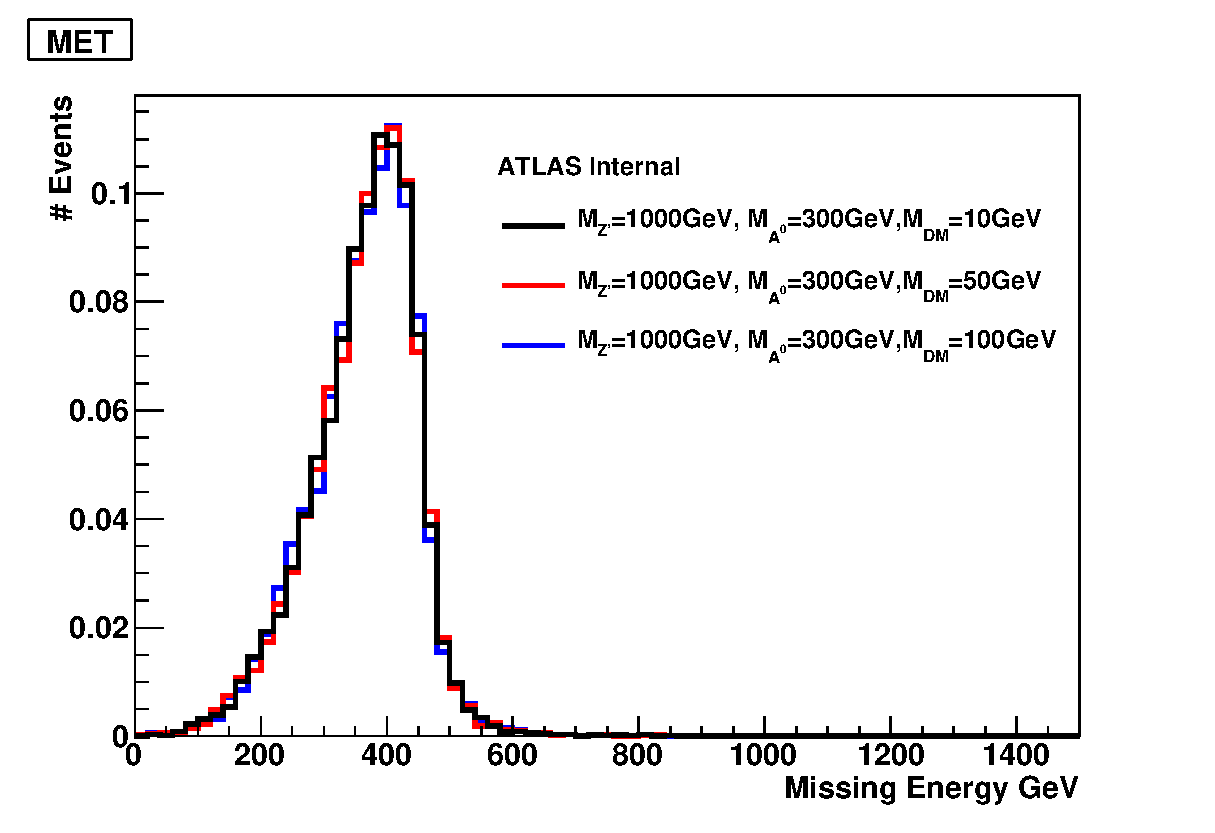
\includegraphics[width=0.47\linewidth]{figures/EW/monoH/2hdm/tanb1zp1000gz08_met}
	}
	\hfill
	\subfloat[$\Delta\phi$ distance between the two $b-$ jets]{
		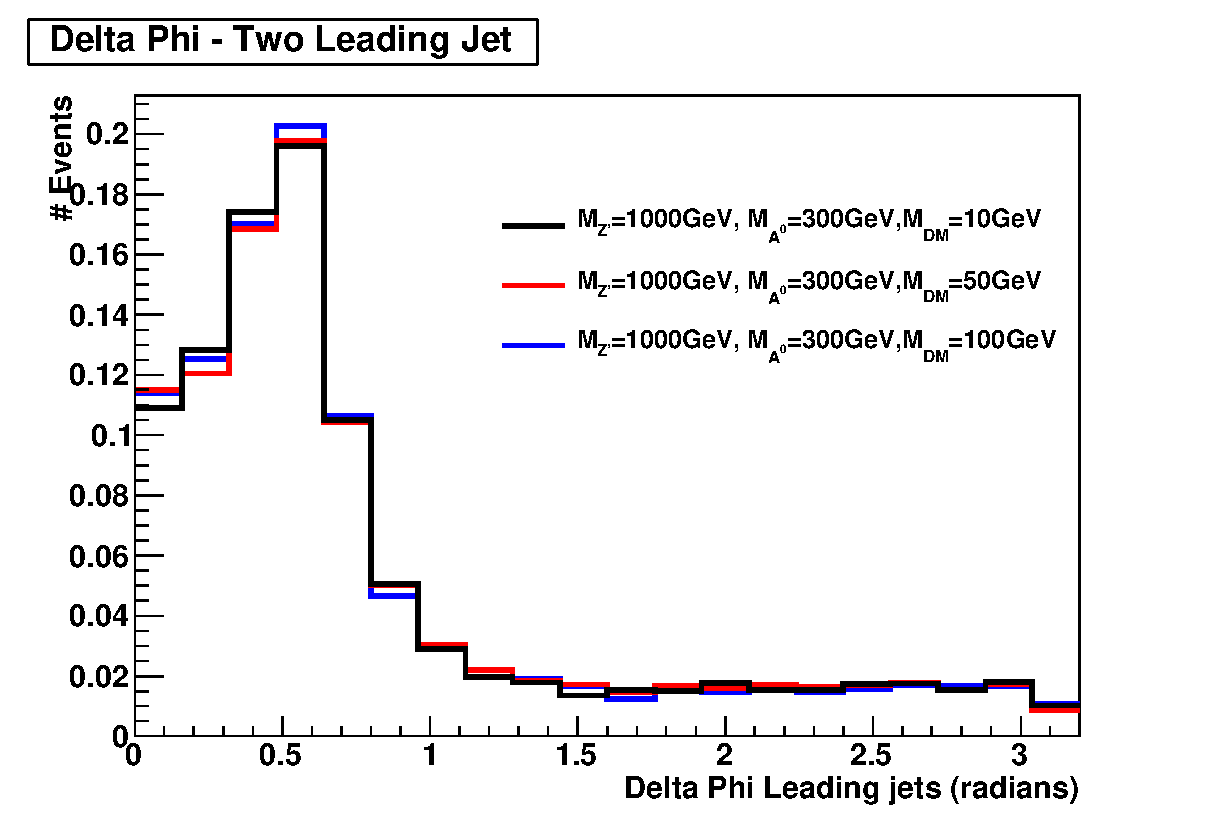
\includegraphics[width=0.47\linewidth]{figures/EW/monoH/2hdm/tanb1zp1000gz08_dphi12}
	}
	\caption{Kinematic distributions of the signal process varying \mDM: minimal kinematic dependency on \mDM as expected when $A^0$ is produced on-shell. Plots shown for $M_{\Zprime}=1000$~\gev, $M_{A^0}=300$~\gev.}
	\label{fig:DMH_mdm}
\end{figure}
 
  \begin{figure}[hbpt!]
  	\begin{center}
  		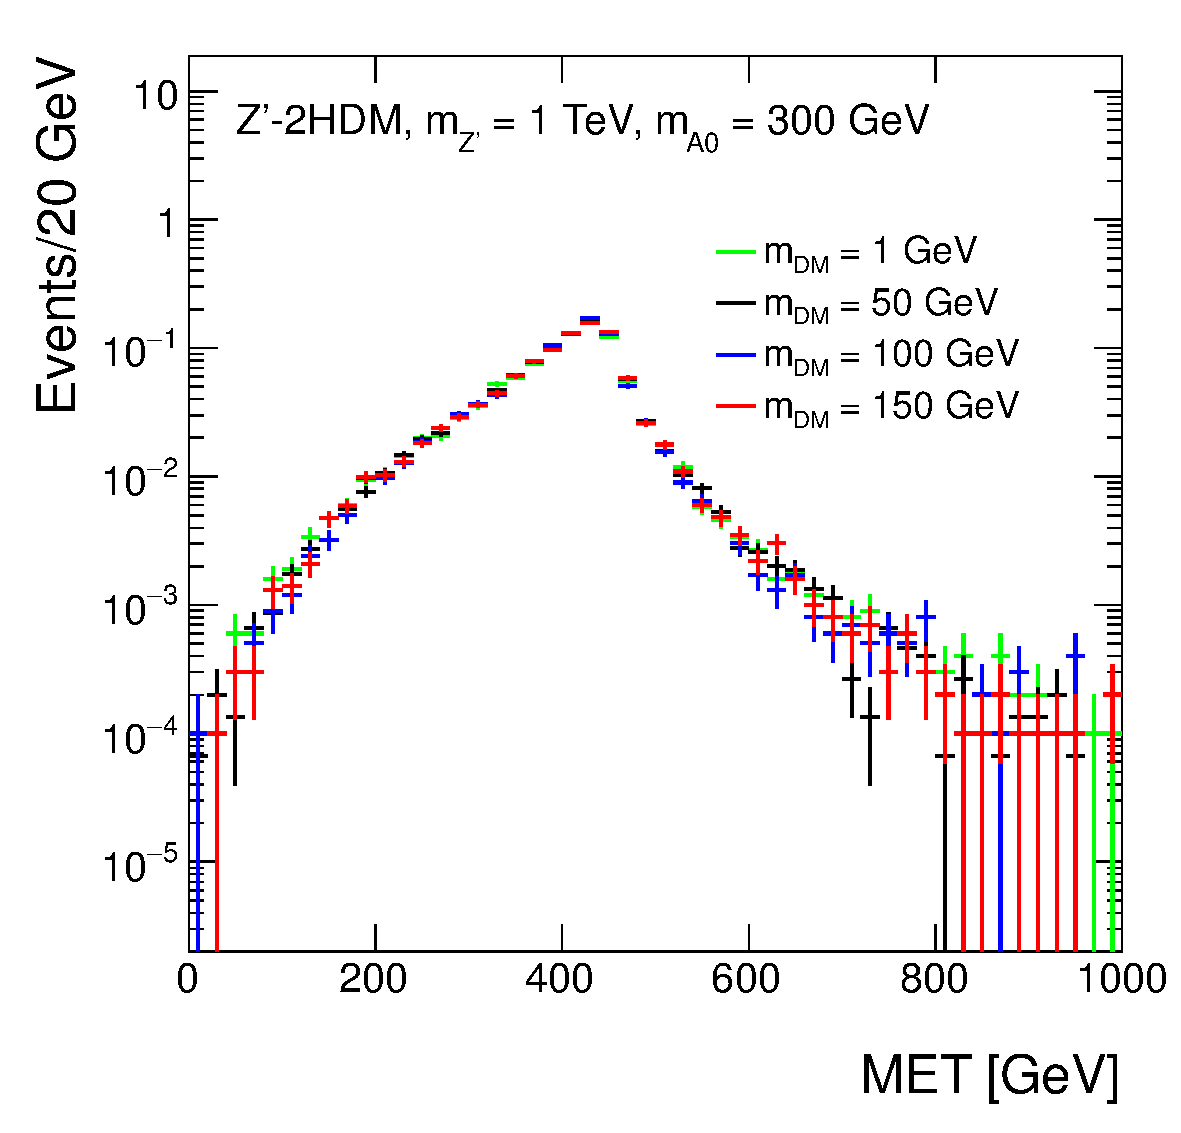
\includegraphics[width=0.49\linewidth]{figures/EW/monoH/zp2hdm_a0_300_MET_et_Log}
  		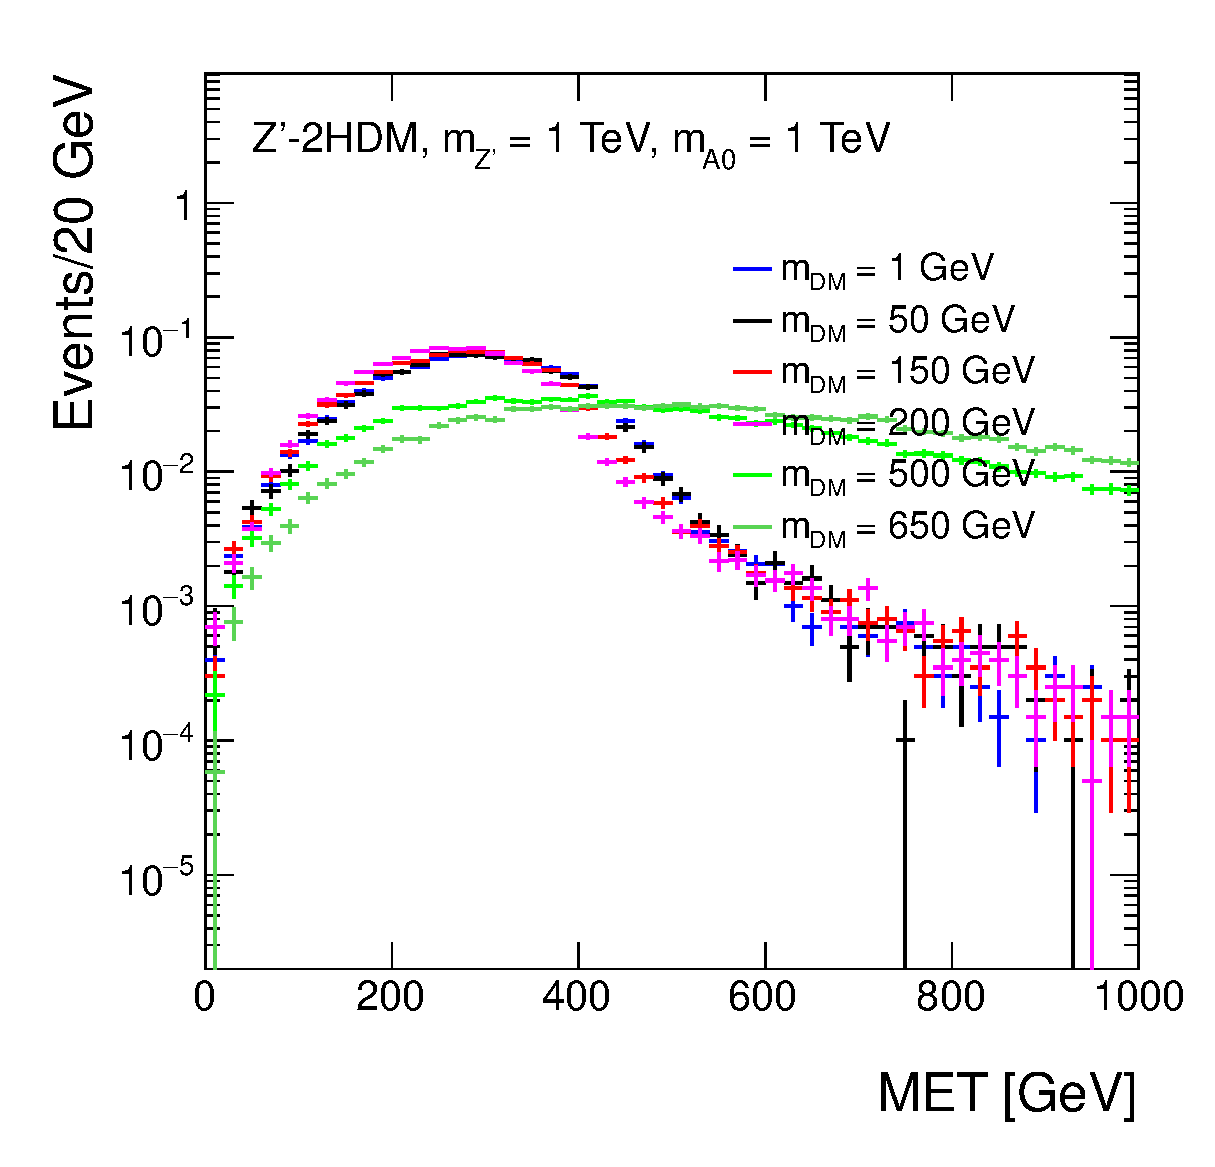
\includegraphics[width=0.49\linewidth]{figures/EW/monoH/zp2hdm_a0_1000_MET_et_Log}
  		\caption{Missing transverse momentum distributions at generator level in the \Zprime+2HDM 
  			scenario for different values of the dark matter mass \mDM, with 
  			$m_{\Zprime}$ = 1~\tev and $m_{A^0}$ = 300~\gev (left) and $m_{A^0}$ = 1~\tev (right).
  			\label{fig:zprimeDecay}}
  	\end{center}
  \end{figure}
  
We recommend to produce signal events for a fixed $g_z=0.8$, $\tan{\beta}=1$ and $\mDM=100$~\gev. For these values, we scan the 2-D parameter space of ${M_{\Zprime}, M_{A^0}}$ with $M_{\Zprime}=600, 800, 1000, 1200, 1400$~\gev, and $M_{A^0}=300, 400, 500, 600, 700, 800$~\gev with $M_{A^0} < M_{\Zprime}-m_h$, for a total of 24 points. The choice of scan is justified by the sensitivity study in~\cite{Berlin:2014cfa}: the expected LHC sensitivity for Run-2 is up to $M_{\Zprime} \sim 1.5$~\tev.
For the parameter scan, the DM mass is fixed to 100~\gev. For two $M_{\Zprime}$, $M_{A^0}$ value sets, we vary the DM mass to obtain sample cross section for rescaling results. 
All LO cross sections for the various parameter scan points are reported in Appendix~\ref{app:EWSpecificModels_Appendix}.
The parameter scan excludes the off-shell region, as the cross-sections are suppressed and the LHC would not have any
sensitivity to these benchmark points in early data. 

The kinematic distributions with varying $M_{\Zprime}$ for fixed $M_{A^0}$ are shown in Fig.~\ref{fig:DMH_mzp}, while the dependency on $M_{A^0}$ is shown in Fig.~\ref{fig:DMH_ma0}. 
  
 \begin{figure}[h!]
 	\centering
 	\subfloat[\MET distribution]{
 		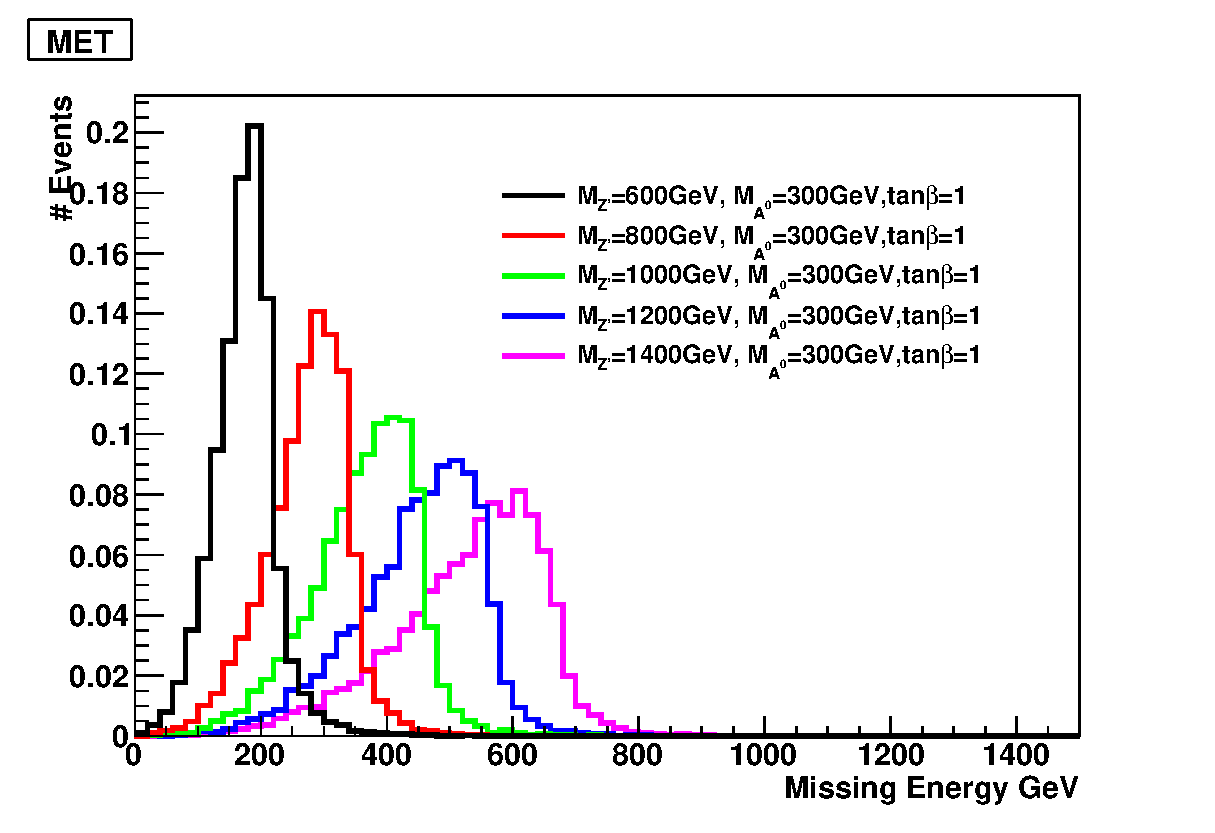
\includegraphics[width=0.47\linewidth]{figures/EW/monoH/2hdm/ZpA0h_tanb1gz08mA300mZp_met}
 	}
 	\hfill
 	\subfloat[Leading $b-$jet $p_T$  distribution]{
 		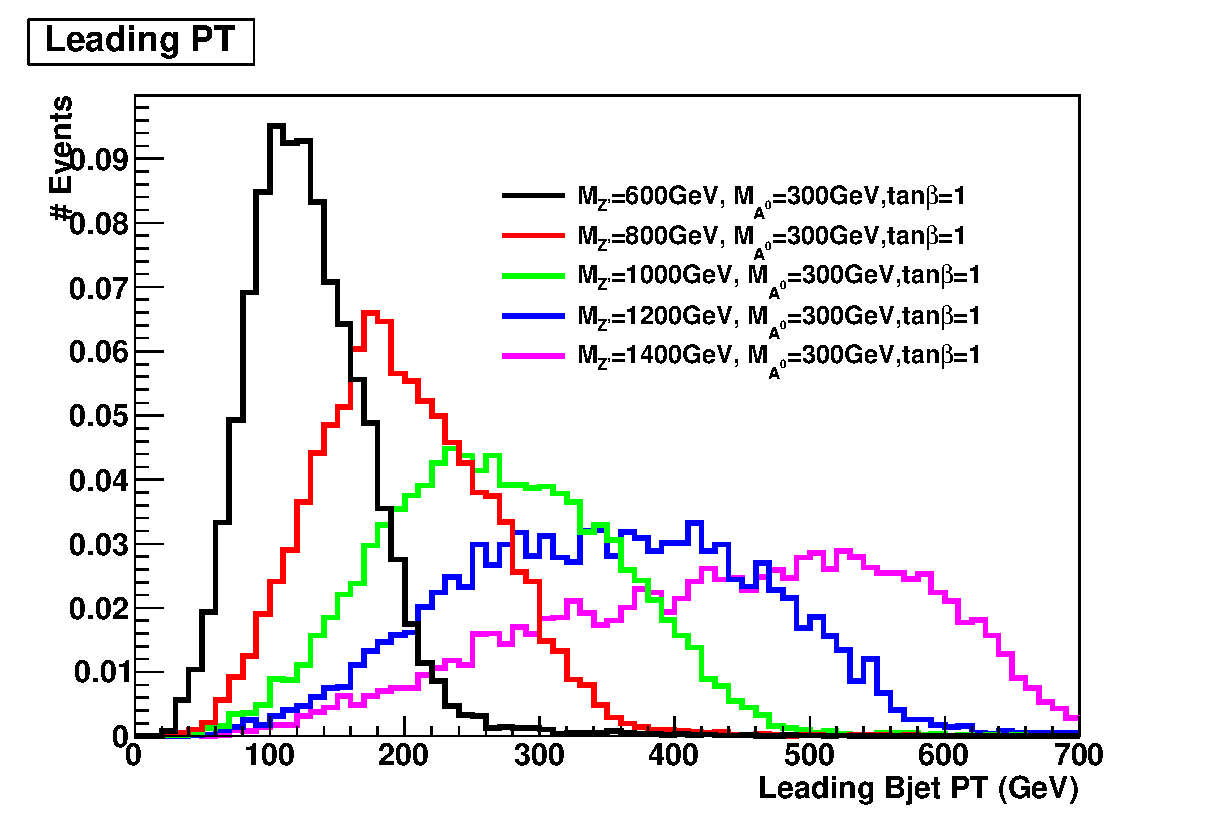
\includegraphics[width=0.47\linewidth]{figures/EW/monoH/2hdm/ZpA0h_tanb1gz08mA300mZp_p0}
 	}
 	\hfill
 	\subfloat[$\Delta\phi$ distance between the two $b-$ jets]{
 		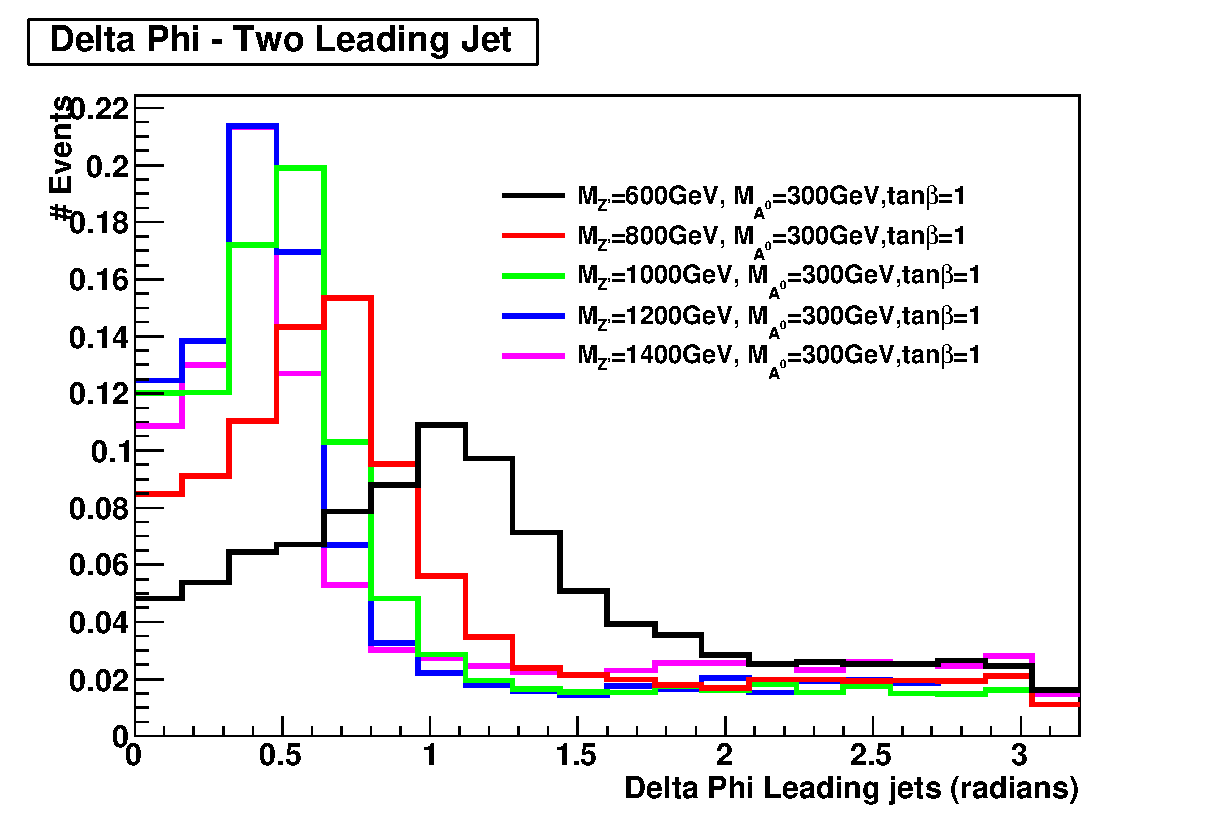
\includegraphics[width=0.47\linewidth]{figures/EW/monoH/2hdm/ZpA0h_tanb1gz08mA300mZp_dphi12}
 	}
 	\hfill
 	\subfloat[Dijet invariant mass]{
 		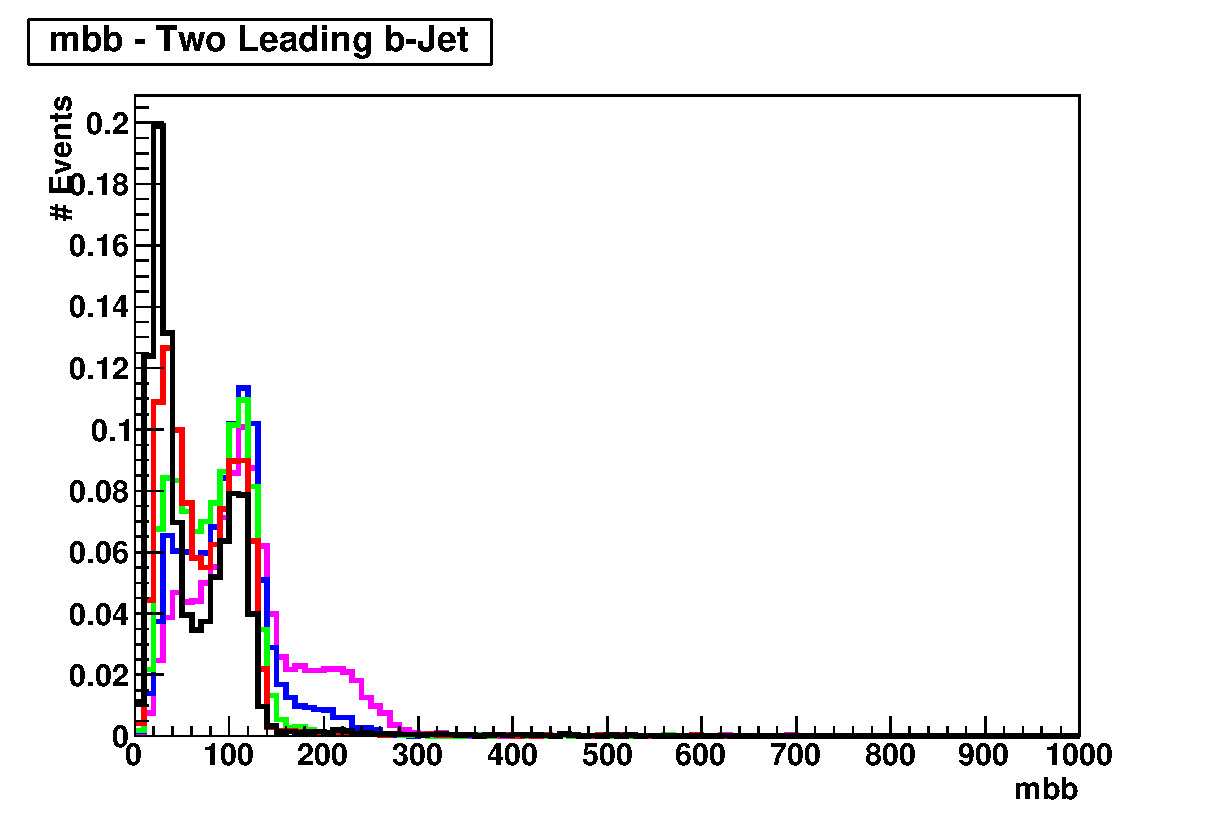
\includegraphics[width=0.47\linewidth]{figures/EW/monoH/2hdm/ZpA0h_tanb1gz08mA300mZp_mbb}
 	}
 	
 	\caption{Kinematic distributions of the signal process varying $M_{\Zprime}$, for $\mDM=100$~\gev, $M_{A^0}=300$~\gev.}
 	\label{fig:DMH_mzp}
 \end{figure}
  
   \begin{figure}[h!]
   	\centering
   	\subfloat[\MET distribution]{
   		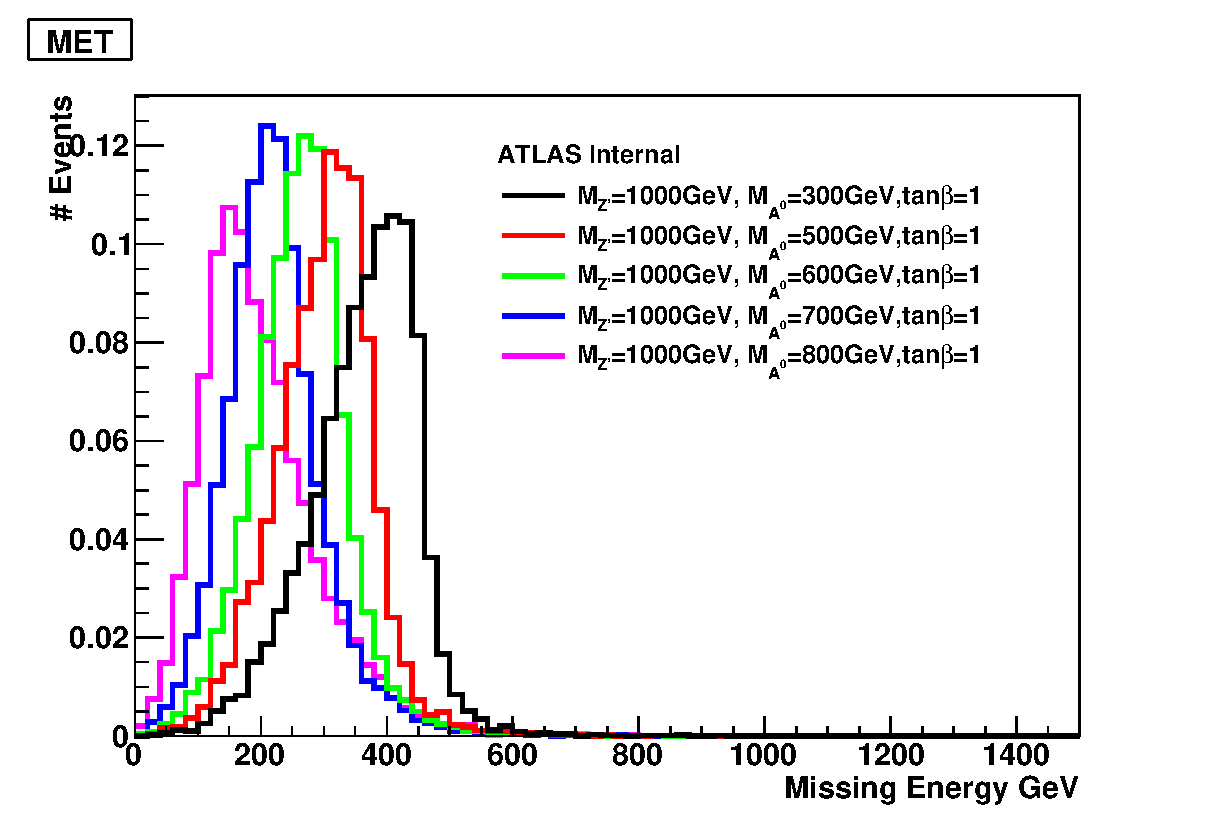
\includegraphics[width=0.47\linewidth]{figures/EW/monoH/2hdm/ZpA0h_tanb1gz08mZp1000mA_met}
   	}
   	\hfill
   	\subfloat[Leading $b-$jet $p_T$ distribution]{
   		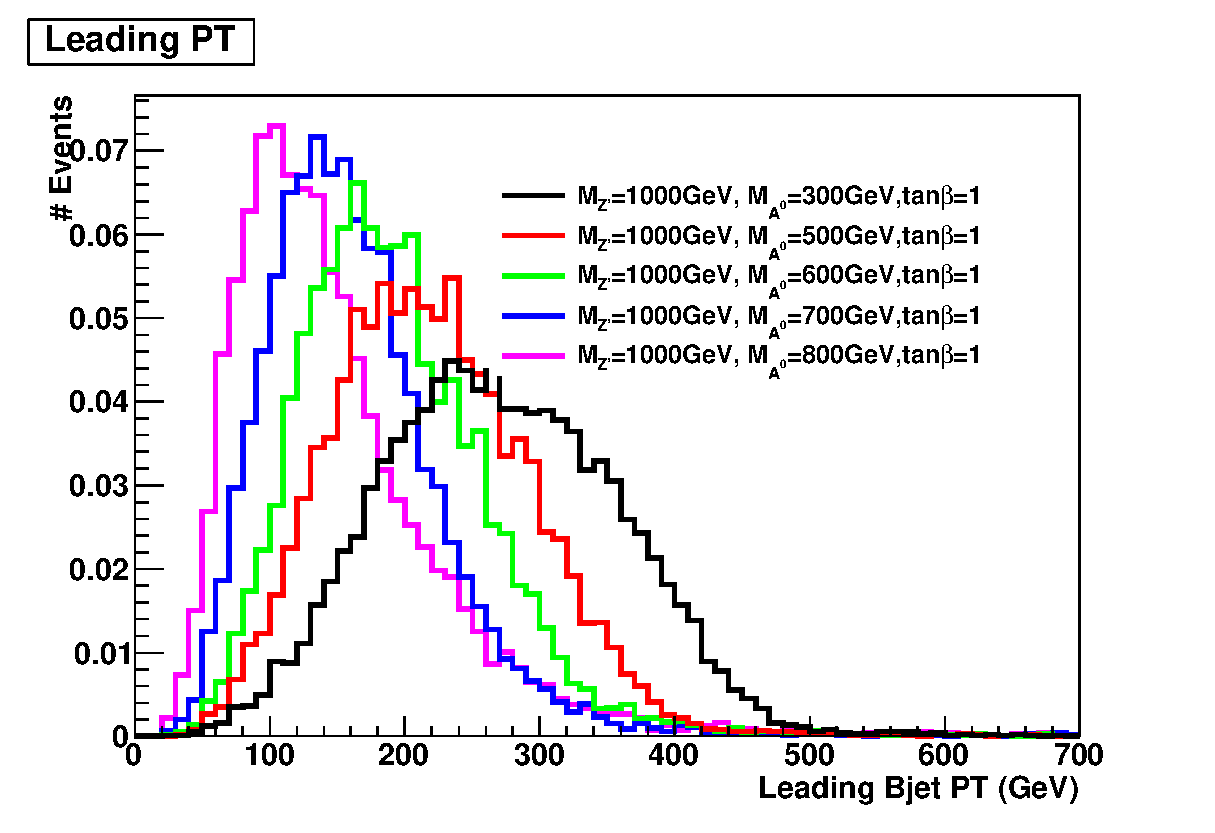
\includegraphics[width=0.47\linewidth]{figures/EW/monoH/2hdm/ZpA0h_tanb1gz08mZp1000mA_p0}
   	}
   	\hfill
   	\subfloat[$\Delta\phi$ distance between the two $b-$ jets]{
   		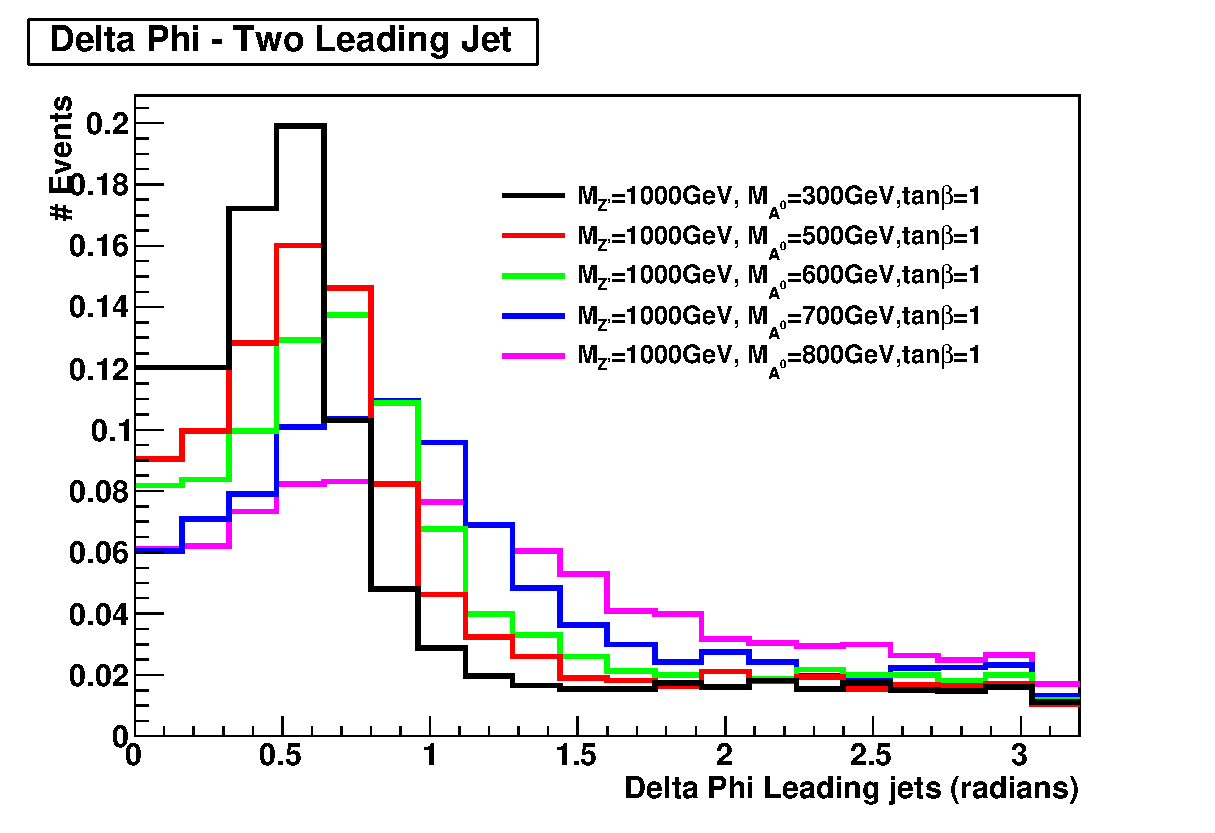
\includegraphics[width=0.47\linewidth]{figures/EW/monoH/2hdm/ZpA0h_tanb1gz08mZp1000mA_dphi12}
   	}
   	\hfill
   	\subfloat[Dijet invariant mass]{
   		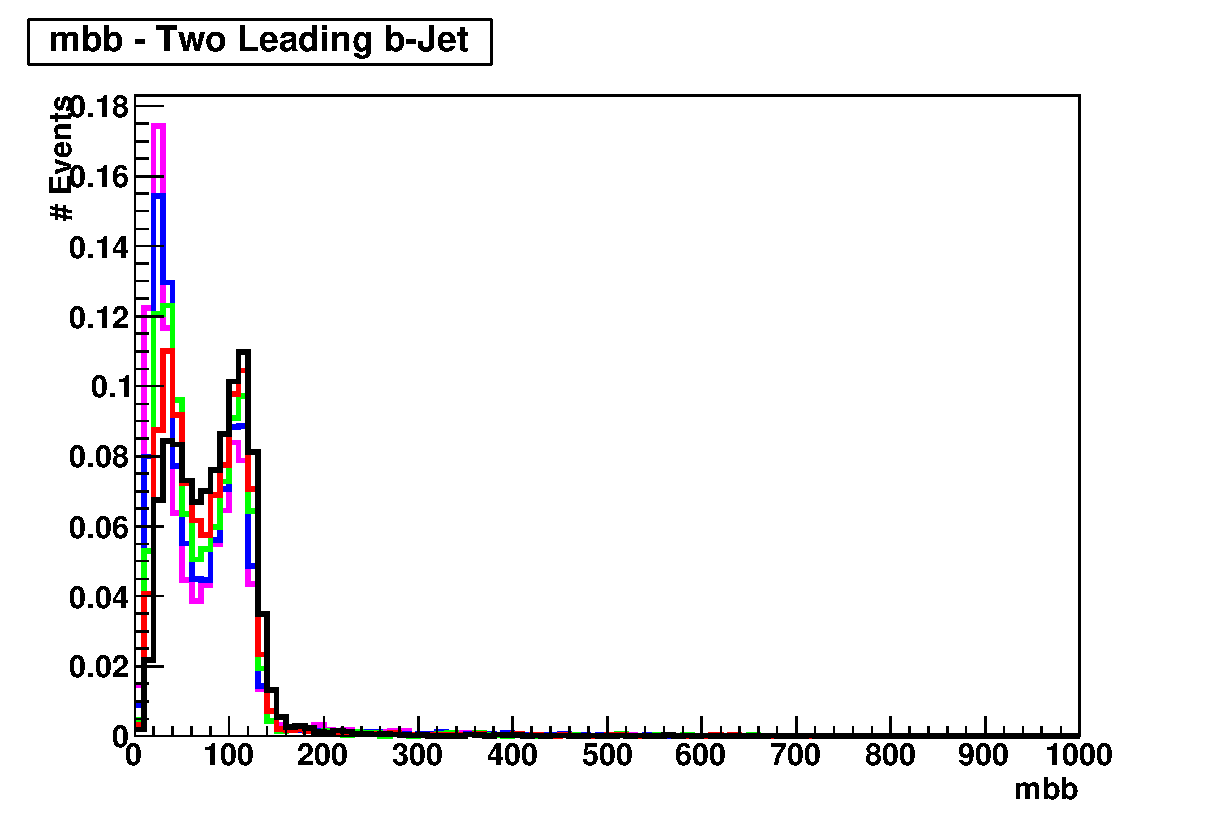
\includegraphics[width=0.47\linewidth]{figures/EW/monoH/2hdm/ZpA0h_tanb1gz08mZp1000mA_mbb}
   	}
   	\caption{Kinematic distributions of the signal process varying $M_{A^0}$, for $\mDM=100$~\gev, $M_{\Zprime}=1000$~\gev.}
   	\label{fig:DMH_ma0}
   \end{figure}
      
 This model also allows for an additional source of Higgs plus \MET signal with a similar kinematics (Fig.~\ref{fig:DMH_zpincl}, shown with detector simulation 
 samples) to the signal process from the decay of $\Zprime \to h Z$, where the $Z$ decays invisibly. The partial decay width for the \Zprime is:
 \begin{equation}
 \Gamma_{\Zprime \to hZ}  = (g_z \cos \alpha \sin \beta)^2 \frac{|p|}{24 \pi} \left( \frac{ |p|^2 }{M_{\Zprime}^2} + 3 \frac{M_Z^2}{M_{\Zprime}^2} \right),
 \end{equation}
The values for the \Zprime masses scanned for those samples should follow those of the previous samples, 
namely values of $M_{\Zprime}=600, 800, 1000, 1200, 1400$~\gev.  This signal process has no $M_A$ dependence. 
 
\begin{figure}[h!]
  	\centering
  	\subfloat[\MET distribution]{
  		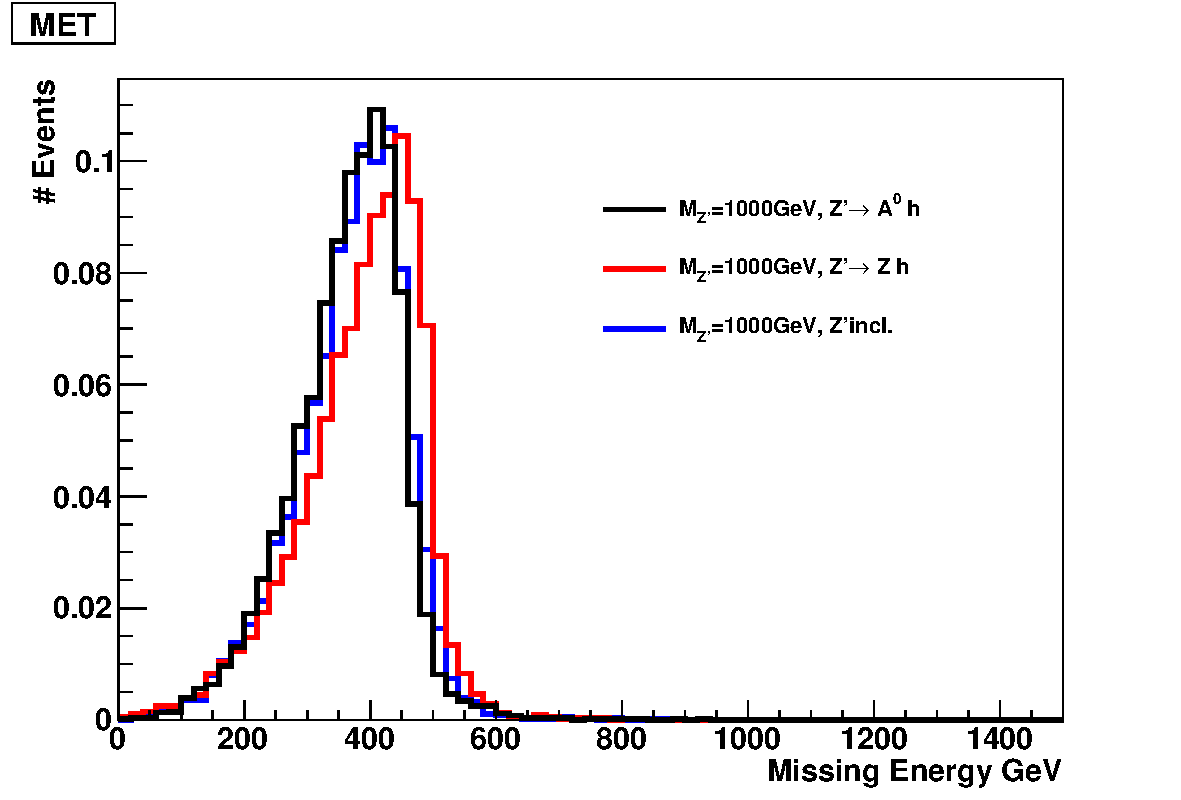
\includegraphics[width=0.47\linewidth]{figures/EW/monoH/2hdm/Zp_tanb1gz08mA300mZp1000_met}
  	}
  	\hfill
  	\subfloat[Leading $b-$jet $p_T$ distribution]{
  		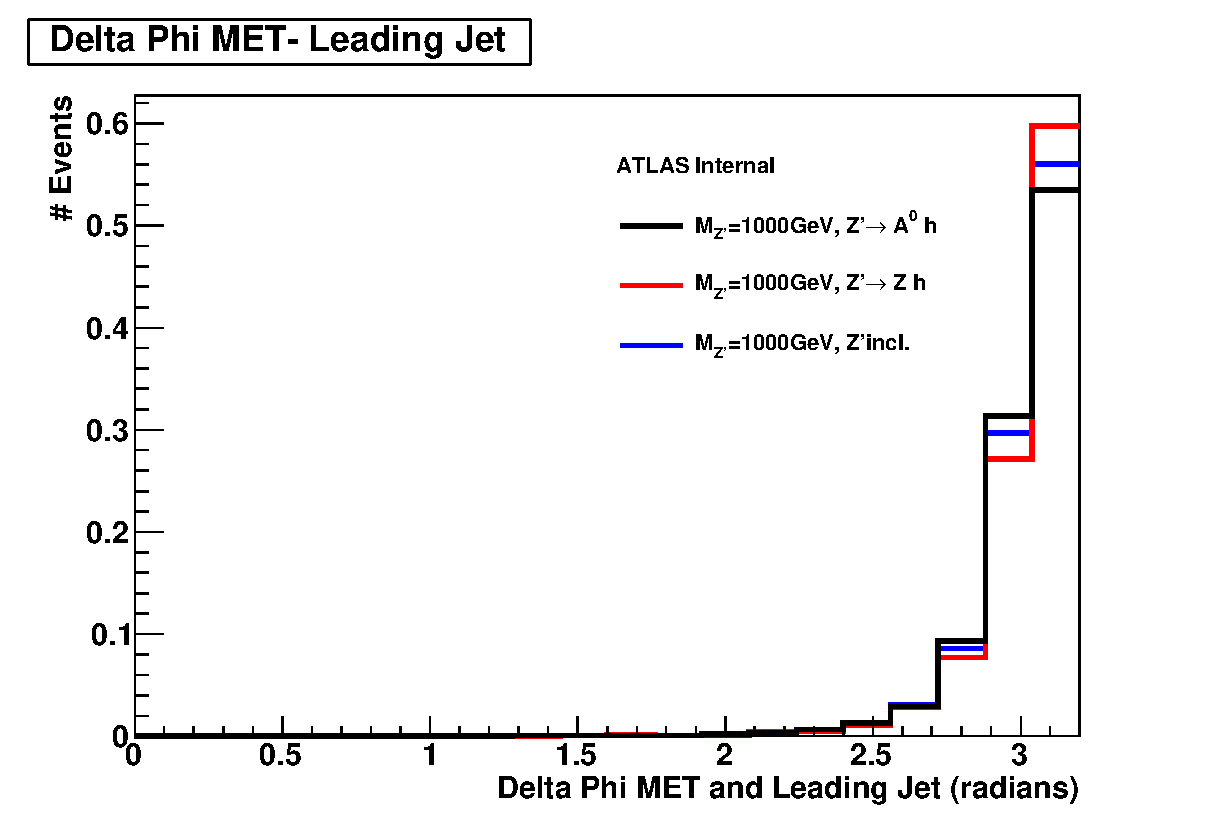
\includegraphics[width=0.47\linewidth]{figures/EW/monoH/2hdm/Zp_tanb1gz08mA300mZp1000_dphimetj0}
  	}
  	\hfill
  	\subfloat[$\Delta\phi$ distance between the two $b-$ jets]{
  		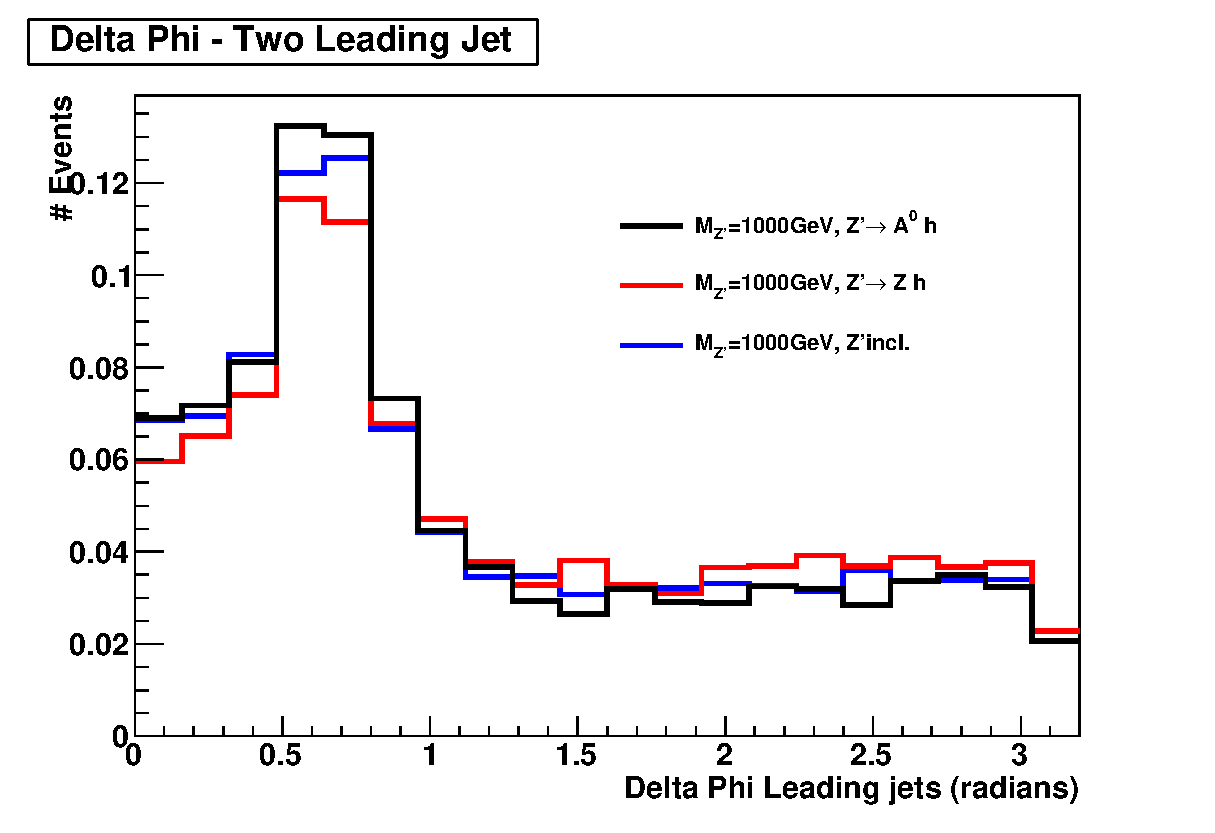
\includegraphics[width=0.47\linewidth]{figures/EW/monoH/2hdm/Zp_tanb1gz08mA300mZp1000_dphi12}
  	}
  	\hfill
  	\subfloat[Dijet invariant mass]{
  		\includegraphics[width=0.47\linewidth]{figures/EW/monoH/2hdm/Zp_tanb1gz08mA300mZp1000_mjj}
  	}
  	\caption{Kinematic distributions of $\Zprime \to A^0\,h$ exclusive production, $\Zprime \to Zh$ exclusive production and \Zprime inclusive production for $M_{\Zprime}=1000$~\gev and $M_{A^0}=300$~\gev}
  	\label{fig:DMH_zpincl}
\end{figure}

\newthought{Implementation discussed in the Appendix}


  
